\documentclass[oneside, 12pt]{book}
\newcommand{\sectionbreak}{\clearpage}


\usepackage{setspace}
% Show page frames.
%\PassOptionsToPackage{showframe}{geometry}

% For test text.
\usepackage{blindtext}
 % TODO: Remove testing packages.
\usepackage[utf8]{inputenc}
\usepackage[driver=pdftex]{geometry}
\usepackage[pagestyles]{titlesec}
\usepackage[linktoc=all]{hyperref}
\usepackage{xcolor}
\usepackage{enumitem}
\usepackage{amsfonts}
\usepackage{graphicx}

\graphicspath{{./assets/img/}}



% Set page geometry.
\geometry{margin = 1in}

% Front and main matters.
\makeatletter
\renewcommand{\frontmatter}{\cleardoublepage\@mainmatterfalse}
\renewcommand{\mainmatter}{\cleardoublepage\@mainmattertrue}
\makeatother

% Chapter title format.
\titleformat{\chapter}{\normalfont\bfseries\Huge}{\thechapter.\enspace}{0pt}{\Huge}
%\newpagestyle{mystyle}{\sethead[\thechapter.][][\chaptertitle]{}{}{\thepage}}
%\pagestyle{mystyle}
\titlespacing*{\chapter}{0pt}{0pt}{40pt}

% Page style.
\pagestyle{plain}


\newcommand{\TODO}[0]{\textbf{\color{red}TODO }}

\newcommand{\appname}[0]{WPI Library }

\doublespacing



\usepackage{multicol}
\renewcommand{\labelitemi}{$\bullet$}
\renewcommand{\labelitemii}{$\color{gray}\bullet$}
\renewcommand{\labelitemiii}{$\circ$}
\renewcommand{\labelitemiv}{\tiny\blacksquare$}

% Document info.
%\title{Mobile App Development For The WPI Gordon Library}
%\author{John Muirhead, Brandon Scanlon, Oliver Yasuna}
%\date{October 2021} % TODO: Update.

\begin{document}
\renewcommand{\BRetrievedFrom}{}

%\maketitle
% \begin{titlepage}
%     \centering
%     {\LARGE\scshape \href{https://www.wpi.edu/}{Worcester Polytechnic Institute}\par}
%     \vspace*{1.2cm}
%     \href{https://www.wpi.edu/}{
\includegraphics[]{assets/img/150px-WPI_logo.png}}\\
%     \vspace*{2cm}
%     \rule{\textwidth}{1pt}\\
%     \vspace{0.5cm}
%     {\huge\bfseries Mobile App Development for the WPI Gordon Library\par} % TODO: Link to Digital WPI.
%     \vspace{0.5cm}
%     \rule{\textwidth}{1pt}\\
%     \vspace{2cm}
%     {\large\scshape Participants} \\[\baselineskip]
%     {\Large
%         John Muirhead\\ % TODO: Link.
%         \href{https://www.linkedin.com/in/brandon-scanlon/}{Brandon Scanlon}
%         \href{https://oliveryasuna.github.io/}{Oliver Yasuna}
%     \par}
%     \vspace{1cm}
%     {\large\scshape Advisor} \\[\baselineskip]
%     {\Large \href{https://www.wpi.edu/people/staff/lostapowiczcritz}{Lori Ostapowicz-Critz}\par}
%     \vfill
%     {\itshape October 2021\par} % TODO: Update.
% \end{titlepage}
\begin{titlepage}
    \centering
    \href{https://www.wpi.edu/}{
\includegraphics[]{assets/img/150px-WPI_logo.png}}\\
    \vspace*{2cm}
    \rule{\textwidth}{1pt}\\
    \vspace{0.1cm}
    {\Large\bfseries Mobile App Development for the WPI Gordon Library\par} % TODO: Link to Digital WPI.
    \vspace{0.1cm}
    \rule{\textwidth}{1pt}\\
    {An Interactive Qualifying Project submitted to the Faculty of WORCESTER POLYTECHNIC INSTITUTE in partial fulfillment of the requirements for the Degree of Bachelor of Science.}
    \vspace{1cm}\\
    \begin{tabular}{c@{\hspace{5em}}c}
        {\large\scshape Participants} & {\large\scshape Advisors}\\
        \\
        Muirhead, John & Ostapowicz-Critz, Lori\\
        Scanlon, Brandon\\
        Yasuna, Oliver
    \end{tabular}
    
    \vfill
%     \begin{multicols*}{2}
%         {\large\scshape Participants\\}
%         \vspace{0.5cm}
%         {\Large Muirhead, John\\} \vspace{0.2cm}
%         {\Large Scanlon, Brandon\\} \vspace{0.2cm}
%         {\Large \href{https://oliveryasuna.github.io/}{Yasuna, Oliver}\\}
%         \vfill
%         \vspace{4cm} % Force "Advisors" into the next column.
%         {\large\scshape Advisors\\}
%         \vspace{0.5cm}
%         {\Large \href{https://www.wpi.edu/people/staff/lostapowiczcritz}{Ostapowicz-Critz, Lori}\\}
%   \end{multicols*}
  Date: March 2022\\
  \vspace{0.5cm}
  \textit{This report represents work of one or more WPI undergraduate students submitted to the faculty as evidence of a degree requirement. WPI routinely publishes these reports on its web site without editorial or peer review.}
\end{titlepage}

\frontmatter
    \tableofcontents
    \chapter{i. Abstract}
        \blindtext

    \chapter{ii. Acknowledgements}
        \TODO

\section*{Development Frameworks \& Libraries}

    \paragraph{Spring}
    Spring, Spring Framework, and their logos are \href{https://spring.io/trademarks}{property} owned by Pivotal Software Inc. These words and logos may exist in this document. In addition, Spring and the Spring Framework were used in software development. They are licensed under the \href{https://www.apache.org/licenses/LICENSE-2.0}{Apache License 2.0}.

    \chapter{iii. Glossary}
        \paragraph{API}  Application Programming Interface
\paragraph{AWS}  Amazon Web Services
\paragraph{CSS}  Cascading Style Sheets
\paragraph{GUI}  Graphical User Interface
\paragraph{HTML} HyperText Markup Language
\paragraph{HTTP} HyperText Transfer Protocol
\paragraph{JSON} JavaScript Object Notation
\paragraph{OS}   Operating System

%---------------------------------------------------------------------------------------------------------------------------------------------------------
\chapter{iv. Authorship}

\begin{table}[ht]
\scalebox{.85}{
\hspace{-0.5in}
\begin{tabular}{| l | l | l | l |}

 \hline
 
 \underline{\textbf{Section}} &  \underline{\textbf{Writer(s)}} &  \underline{\textbf{Editor(s)}}\\\hline \hline

 \textbf{i. Abstract} &  \textbf{} &  \textbf{} \\ \hline \hline
 
 \textbf{ii. Acknowledgments} &  \textbf{} &  \textbf{} \\ \hline \hline
 
 \textbf{iii. Glossary} &  \textbf{} &  \textbf{} \\ \hline \hline

 \textbf{iv. Authorship} &  \textbf{Brandon Scanlon} &  \textbf{All} \\ \hline \hline
 
 \textbf{1. Introduction} &  \textbf{Oliver Yasuna} &  \textbf{Brandon Scanlon} \\ \hline \hline

 \textbf{2. Literature Review} &  \textbf{All} &  \textbf{All} \\ \hline
  2.1 Introduction & Brandon Scanlon & Brandon Scanlon \\ \hline
  2.2 Significance of Topic & Brandon Scanlon & Brandon Scanlon \\ \hline
  2.3 Known and Unknowns & Oliver Yasuna & Brandon Scanlon \\ \hline
  2.4 Current Models in This Field of Study & Oliver Yasuna & Brandon Scanlon \\ \hline
  2.5 State of the Art & John Muirhead & John Muirhead \\ \hline
  2.6 Relation to the Larger Problem Area & John Muirhead & John Muirhead \\ \hline
  2.7 Closing Thoughts & All & Brandon Scanlon, (*ADD*) \\ \hline \hline

 \textbf{3. Methodology} &  \textbf{All} &  \textbf{All} \\ \hline
  3.1 Introduction & John Muirhead & John Muirhead \\ \hline
  3.2 Needs Analysis & Brandon Scanlon & Brandon Scanlon \\ \hline
  3.3 Functions (Specification) & Brandon Scanlon & Brandon Scanlon \\ \hline
  3.4 Conceptual Designs & Brandon Scanlon & Brandon Scanlon \\ \hline
  3.5 Preliminary / Alternative Designs & Oliver Yasuna & Brandon Scanlon \\ \hline
  3.6 Feasibility Study & Oliver Yasuna &  \\ \hline
  3.7 Modeling & Oliver Yasuna &  \\ \hline
  3.8 Preliminary Findings / Outcomes & John Muirhead &  \\ \hline
  3.9 Final Design Strategy & John Muirhead &  \\ \hline
  3.10 Techniques for Deployment & John Muirhead &  \\ \hline \hline
 
  \textbf{4. Results} &  \textbf{Brandon Scanlon, Oliver Yasuna} &  \textbf{Brandon Scanlon, Oliver Yasuna} \\ \hline
  4.1 Introduction & Oliver Yasuna & Oliver Yasuna \\ \hline
  4.2 Student Survey & Brandon Scanlon & Brandon Scanlon \\ \hline
  4.3 Technical & Oliver Yasuna & Oliver Yasuna \\ \hline \hline
  
  \textbf{5. Conclusion} &  \textbf{} &  \textbf{} \\ \hline
  
  \hline \hline
  
  \textbf{6. Recommendations} &  \textbf{} &  \textbf{} \\ \hline
  
  \hline \hline
  
  \textbf{7. Appendix} &  \textbf{Brandon Scanlon, John Muirhead} &  \textbf{Brandon Scanlon, John Muirhead} \\ \hline
  7.1 Timeline & Brandon Scanlon & Brandon Scanlon \\ \hline
  7.2 Additional App Research & John Muirhead & John Muirhead \\ \hline
  7.3 Academic Library Features & Brandon Scanlon & Brandon Scanlon \\ \hline
  7.4 Student Survey & Brandon Scanlon & Brandon Scanlon \\ \hline
  7.5 Survey Results & Brandon Scanlon & Brandon Scanlon \\ \hline \hline
  
\textbf{References} &  \textbf{All} &  \textbf{John Muirhead} \\ \hline
  
\hline
\end{tabular}
}
\end{table}
%---------------------------------------------------------------------------------------------------------------------------------------------------------
\mainmatter
    \chapter{Introduction}
        

\paragraph{}
The overall use of handheld devices has increased dramatically within the past decade or so, especially in academic practices. As technology grows, our environment adapts to such changes. However, to keep up with the advancements of technology is no simple task and public services can fall short. The WPI George C. Gordon Library, for instance, offers high quality information resources, expert consultations and instructional services, and a variety of work spaces to support the WPI community. Students can utilize the library for its quiet study spaces, private group study rooms, research consultations, and more. On the technical side, the library staff is able to provide their services through a handful of different systems. These resources, on the other hand, are made available strictly on web-hosted applications, requiring a web browser. This is quite cumbersome and not user friendly on mobile devices whatsoever as a mobile website is merely a stripped-down version of the source web page. In our world, where convenience is key, the student demographic as turning away from using the library services.

\paragraph{}
As few steps had been taken towards improving the accessibility of such services, this project aimed to produce a mobile-first web application, centralizing many library services into one place to cater to mobile devices and promote convenience. We believed that by establishing a fully functioning mobile application, the ”traffic” to the library’s resources and services would increase, along with the foot traffic within the Gordon Library building.The expansion of other requested services, such as individual computer occupancy tracking so that users can know how many computers are available at a given time, and a remote book check-out service were beyond the scope of this IQP project.

\paragraph{}

    The Progressive Web Application (PWA) standard was utilized for the development of the mobile application. This means that our application meets the following criteria:
    
   \begin{itemize}[label={\checkmark}]
       \item Progressive  -- Works for most users on most devices and web browsers.
      \item Responsive   -- User interface (UI) fits any common form factor: desktop, table, mobile.
     \item App-like     -- Feels and acts like a native mobile app on mobile devices.
        \item Safe         -- Content served via encrypted HTTPS to secure user accounts and interactions.
        \item Discoverable -- Identifiable as a website, found on search engines.
        \item Installable  -- Able to be added to a mobile device's homescreen as a normal app.
        \item Linkable     -- Easily shared via a URL and does not require complex installation.
    \end{itemize}

\paragraph{}

    The PWA standard is still being adopted by some browsers and devices. At the time of the \appname app development, support for every feature may not be available to all users, depending on device and browser.

        
    \chapter{Literature Review}\label{ch:lit_rev}\addcontentsline{toc}{chapter}{Literature Review}
        %2.1 -- INITIAL REVISIONS MADE
\section{Introduction}
\paragraph{}
Within this chapter, we share an overview of the problem pertaining to the library resource's mobile capabilities, academic and otherwise. We will describe the pros and cons, as well as the possible solutions. Next, we delineate best practices related to mobile application development that have been refined and certified by experts within this field. To conclude, we introduce the requirements to develop a mobile application from the ground up.


%2.2 -- INITIAL REVISIONS MADE
\section{Significance of the Topic}
\paragraph{}
 Our world is becoming more and more reliant on devices such as our mobile phones. These mobile devices unlock a connection between the user and a vast and seemingly endless supply of helpful and sometimes not so helpful resources. With this in mind, this connective architecture, according to Yip et al., "serves as a virtual platform for learners to engage with their learning activities in a more spontaneous, personal, informal, contextual, portable, ubiquitous and pervasive way" (2021, p. 389). Mobile applications are greatly utilized in the academic world on all levels. From elementary school to college graduate students, such applications aid each one to some extent, broadening their learning capabilities and resources.
 
 \paragraph{}
 Mobile apps can often emulate desktop-based websites, but are streamlined in comparison. The use of this is to take a website that is accessible through a desktop or laptop and enable the same or more stark access to the same website. While developing a mobile website that could house the resources of a library may be a more simple task, it leaves for less capabilities and utilities for the mobile user. Developing a native application that can support any mobile platform is a more daunting task, however, the results are of a much higher quality in the end. The user experience in this case is far superior to that of a website (Margam \& Saleeq, 2017, p. 110).
 
\paragraph{}
 Shih-Chuan Chen states, based on the results from a survey of undergraduate students, "Many libraries provide mobile app services because of the rapid increase in smartphone users" (2019, p. 731). He also goes on to note how many elementary tasks are accomplished more efficiently on a mobile device than on a computer, however, the inverse is true for tasks that require the use of searching and web browsing. Laptops and desktops alike were proven to supersede mobile devices in this case, however, mobile devices are still useful for these tasks. This survey shows that, having academic options such as mobile resources that are engaging and user friendly could negate the necessity of in-person attendance to a library or other academic facility. Certain resources such as occupancy tracking, tech suite booking, library hours, and others would not only help students to use their time more efficiently, and potentially reduce the number of people in the library and thereby help follow any local social distancing guidelines in a safer manner.
 
 \paragraph{}
 After all, we live in a time where convenience is of utmost importance. No one of us desires to wait for access to something we need to use. It is a natural human behavior. Technology has amplified that mentality as it provides its users relatively instant access to just about anything at anytime (Shahriza et al., 2006).

\paragraph{}
When developing a mobile application, many factors have to be considered well in advance before code starts to be structured and written. For example, a native application is typically developed to be supported on a specific device platform such as IOS devices. Thus, when developing a mobile app, additional steps need to be taken to include the possibility that the app can be supported by all or most other mobile devices as well. After development, the application will need to be verified and reviewed by the various app stores, i.e. Android's Google Play Store and Apple's App Store, to be displayed and downloadable for any user on each respective platform. Since the application is intended to be public and accessible by many, it has to be run on a network server (Huy \& vanThang, 2012, p. 25-26). These App stores have a significant amount of user traffic, and billions of application downloads and dollars in revenue have transpired on just the Apple App and Google Play stores. These conditions make for a seriously competitive industry (Wang et al., 2017, p. 163).

\paragraph{}
Acknowledging the features a mobile application should embody can be relatively easy, but determining the delivery format and final product in which the user consumes such an app is far more difficult. In a study conducted by Ngu Phuc Huy from Norwegian University of Science and Technology and Do vanThanh from Telenor \& Norwegian University of Science and Technology, four different types of mobile app paradigms were analyzed: Mobile native applications, Mobile widgets, Mobile Web applications, and HTML5 mobile applications. From their research, Huy and vanThanh devised what they called "Evaluation Criteria" (\url{https://doi.org/10.1145/2428955.2428968}) which outlines a rigorous and detailed template for mobile app development (2012, p. 26-27). This evaluation criteria spells out the necessary steps, some perhaps unnecessary in some cases, that aid a developer in structuring and designing a mobile application. Each criterion is carefully considered in the development process to deliver a product to the selected demographic in the best and most effective way possible.



%2.3 -- INITIAL REVISIONS MADE
\section{Known and Unknowns}

    \paragraph{}
    Any experienced programmer can effortlessly throw together a quick application, but developing a user-facing application that people will want to use is entirely another beast. A development team requires more resources, such as designers for the look-and-feel of a mobile application. This also applies to the development of a mobile library application. According to Saragossi et al., "the adoption of mobile apps as an emerging format within the Libraries’ collections necessitates a varied outreach strategy that endeavors to make apps accessible and approachable" (2018, p. 202). So, how does one design and implement an accessible and approachable mobile application? Through research. This research includes, surveys and credible sources to provide evidence and a concrete background that will lead the reader to the point in which the team's work will embark.
    
    Shih-chuan Chen, a professor of Library and Information Sciences, researched the potential benefits for students when using mobile applications to search library catalogs. The study "demonstrates that the participants spent more time completing tasks while using the laptop than that they did while using the mobile app" (Chen, 2019, p. 727). This research clearly shows that users can be more efficient on a mobile device, specifically in the case of utilizing academic library resources.
    
    However, not all features of applications are best used on mobile devices. For example, the same study proved that: \begin{quote} ten participants [out of 16 undergraduate students] reported that it was easier to search the library catalog using the laptop. They explained that they were familiar with the interface of web OPACs [library catalog], and more information was displayed. Moreover, the web OPAC offered more functions. (Chen, 2019, p. 728)\end{quote}
    
    
 %2.4 -- INITIAL REVISIONS MADE
\section{Current Models in This Field of Study}
    \paragraph{}
    A 2018 study by Mansouri and  Soleymani, investigated the necessary features for a library mobile application. The research was performed at the University of Isfahan, known for science, humanities, and engineering.
    \begin{figure}[H]
        \centering
        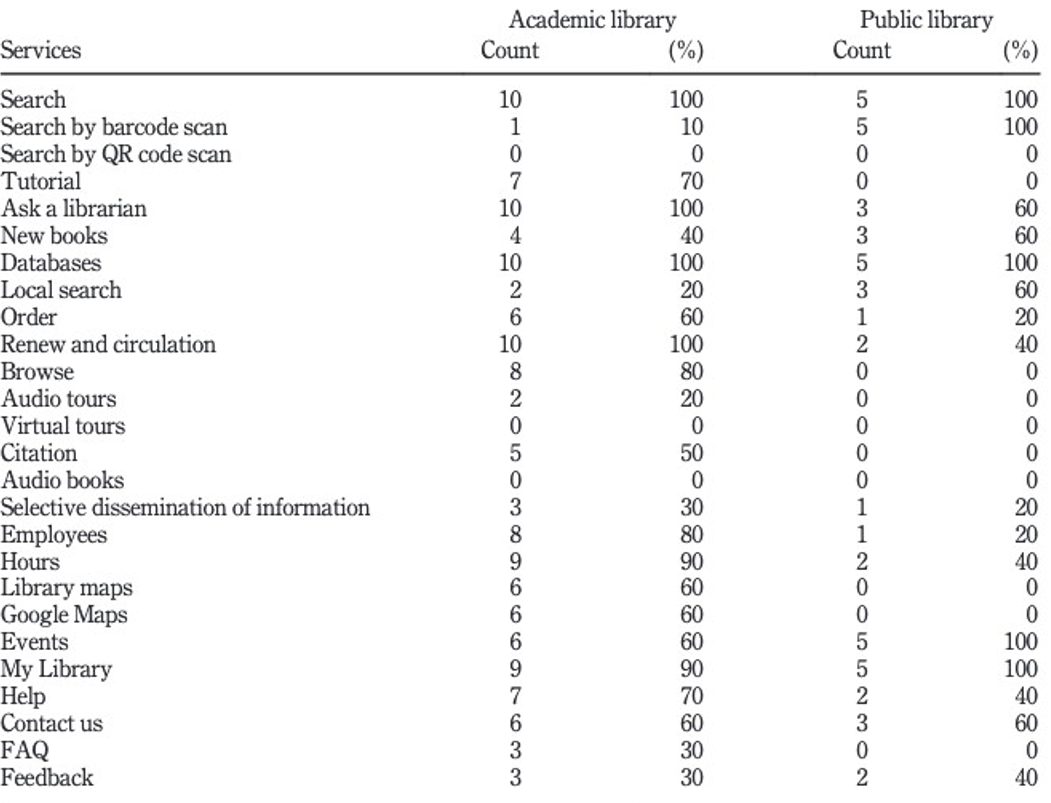
\includegraphics[width = \textwidth, height = \textheight, keepaspectratio]{assets/img/Accessing Mobile Applications.png}
        \caption{Frequency and percentage of components in library mobile applications by type of library}
        \label{fig:freq_and_per_comp_lib_mob_app}
    \end{figure}
    \noindent{} \textit{Note}: From “Assessing mobile application components in providing library services,” by A. Mansouri and N. Soleymani Asl, 2019, \textit{The Electronic Library}, 37(1), p. 53 (https://doi.org/10.1108/EL-10-2018-0204). Copyright 2019 by Emerald Publishing Limited. Reprinted with permission.
    
    
    \paragraph{}
    Figure 2.1 shows the breakdown of all services found within the library mobile applications reviewed by the study, and how frequently they were utilized. The "Public library" column is irrelevant in this report. This is a great example of a model for features that are used in the field already. Such features (see Appendix 6.3.2 for a detailed outline of each) include a search, either by barcode or QR code or both. This enriched set of features was made a common resource within each of the library applications reviewed in this study. Tutorials to help viewers to learn the platform and its capabilities for those who are perhaps new to it are yet another useful feature. The ask a librarian resource would bridge the gap between a librarian and an individual who may have questions for a librarian. A simple, yet helpful feature quite commonly seen in other library applications is the library hours. Having access to the hours of a library provides the users with much of the information they should need to utilize it. The remaining details that may be missing from the user's knowledge would be event and calendar information. Nearly every library mobile app reviewed in this study by Mansouri and Soleymani, provides such a feature. Lastly, a FAQ (Frequently Asked Questions)/Feedback element, not quite as commonly included within a library mobile application, was considered useful nonetheless.
     

%Section 2.5
\section{State of the Art}
    \paragraph{}
    Throughout the years, app development has improved in both efficiency, quality, and accessibility. As a result, library apps - as well as similar learning-based apps - have improved in these criteria congruently. One feature of modern day mobile applications is an emphasis on integration with other relevant software. For example, an Ex Libris press release about the Libris CampusM Mobile App, stated: "The flexibility of the app enables it to be integrated with learning management systems such as Blackboard®, Canvas, and Moodle™"(Ex Libris, 2017). This cross-platform paradigm is essential in applications which were built to service existing technologies and state of the art library mobile applications, and integrate with existing programs and databases. Pu et al. (2015) describes the origins of a library mobile app; "A number of libraries gradually sensed this trend and combined their services with mobile technology to created so-called Mobile Library or M-Library".(2015, p.15-31).
    \paragraph{} 
    In addition to being highly integrated with existing technology, state of the art mobile applications utilize technologies built into smartphones in order to give users the best possible experience. Hu & Neamtiu (2016) state, "The behavior of smartphone apps is driven by input from sensors such as GPS, microphone, or camera" (p.50-56). State of the art library applications also utilize the technology provided by mobile phones in order to maximize their utility. For example, a library app might use the camera in order to scan bar codes. Furthermore, a library application could utilize the GPS technology to inform users about their distance from the library. Essentially, state of the art apps, including library apps, utilize the state of the art technology features on smartphones.
    \paragraph{}
    Another feature of modern technology, particularly software, is change. State of the art applications are dynamic entities; they improve with time and require consistent maintenance (Hu \& Neamtiu, 2016). Anand et al. (2020) writes, "Thus, to keep the software and its data safe, software developers perform continuous testing of the product in its operational phase and release software upgrades or software updates/patches to fix any uprising issue and to improve it (p.1071-1085).  Essentially, state of the art software, mobile applications specifically, including library applications, are upgraded, maintained and modified on a regular basis.
    \paragraph{}
    Yet another feature of state of the art software is the ability to provide value in multiple ways. State of the art tools not only provide useful services to the clients, but also provide the client with value. With respect to library application specifically, this means the software is designed such that data can be collected from the users to exponentially improve the software. Chen (2019) notes, "This indicated that Mobile Library has become a vital resource for learners to acquire knowledge" (p.721-734).
    
    %%List here is just for information purposes. Text above is the actual thing
    
    % \begin{itemize}
    
    %     \item
    %     "The flexibility of the app enables it to be integrated with learning management systems such as Blackboard®, Canvas, and Moodle™" \cite{campusM}
    %     \item
    %     "Since the app runs on library-developed open-source software, feedback from academic users during the pilot program – currently running until August 31 – will also help develop and improve new functionality in the app, which will benefit all library users." \cite{NYU_Library}.
    %     \item
    %     "Since the app runs on library-developed open-source software, feedback from academic users during the pilot program – currently running until August 31 – will also help develop and improve new functionality in the app, which will benefit all library users." \cite{NYU_Library}.
    %     \item 
    %     "The behavior of smartphone apps is driven by input from
    %     sensors such as GPS, microphone, or camera", 
    %     "First, we fuzz (alter) the log in a semantically-meaningful way: by applying 
    %     principled transformations (e.g., changing GPS coordinates
    %     or navigation speed), a new input log is constructed, which
    %     represents a new test case. Second, we use the log captured
    %     in app A to test an app B which offers similar functionality,
    %     e.g., GPS navigation or image recognition"
    %     "For example, GPS allows apps such as Yelp to provide location-aware services; the camera allows image matching apps like Google Goggles to provide search-by-picture features; the Shazam app can help recognize an ambient song by using the microphone."
    %     \cite{FuzzyAndCross}
    %     \item
    %     With the unceasing advancement of mobile technologies, mobile devices developed rapidly. Thus, learning activities could be proceeded anytime and anywhere (Lai et al. , 2014). Wang et al. (2012) indicated that, with the popularization of 3G mobile technologies, more people gained access to internet to view web site, receive and send e-mails and read e-books with smartphones and tablet PCs on metro, bus or train. It could be inferred that learning activities no longer limit to classroom or scheduled time. By combining mobile devices and wireless technology, learning guidance and feedbacks could be given according to learners' learning situations and learning environment (Huang et al. , 2014).

    %     A number of libraries gradually sensed this trend and combined their services with mobile technology to created so-called Mobile Library or M-Library. In fact, the concept of Mobile Library or M-Library was brought up by scholars when PDAs were still in development. For instance, Janet (2009) adapted mobile technology and combined PDA with library orientation and collection search services. However, at that time, mobile devices and wireless technology were not mature and popular.
        
    %     "Recently, mobile technology combined with mobile devices has become an important information collecting channel. A greater number of students and teachers also use tablet PCs and smartphone to search for e-journals, e-books and other e-resources (Parsons, 2010). Therefore, numerous libraries introduced mobile technology in library services and developed mobile information systems compatible to mobile devices in order to allow their users quickly search for desired information (Wang et al. , 2012). This indicated that Mobile Library has become a vital resource for learners to acquire knowledge."
    %     "Ten participants reported that it was easier to search the library catalog using the laptop.They explained that they were familiar with the interface of web OPACs, and more information was displayed on the computer screen than the tablet screen"
    %     "Some participants reported that they would use the smartphone app to search library catalogs when it was inconvenient to use laptops or desktop computers, such as on the bus or in classroom"
    %     \cite{given_one}
       
    % \end{itemize}
    
    
% Section:
% 2.6
\section{Relation to the Larger Problem Area}
    \paragraph{}
     As the world becomes more digitized, and tools once only accessible in person are made accessible via the internet, projects such as this become increasingly relevant. One particular field in which modernization is occuring is mobile development. Specifically, mobile development with respect to the virtualization of already existing tools. This includes mobile apps to make delivery placements for food, mobile applications to handle transportation, and generally any service that can be digitized. According to Genuitec, an enterprise-consulting company, "The open-source community is helping to rapidly advance mobile Web application development. To date, no less than eighteen different mobile frameworks exist just for the iPhone" ("MobiOne Developer 1.0 M4", 2009). Mobile application is one of the broadest and most widely used examples of the digitization of the modern world. 
     
     \paragraph{}
     A number of factors explain this trend towards digitization via mobile applications. Firstly is the decreased cost. A major advantage of software is its repeatability. If software is developed once, it could be re-implemented as many times as desired with virtually no additional cost. Furthermore, mobile applications save users a significant amount of time; virtually any good or service is a few clicks away. Another factor in the popularization of mobile applications is the popularity of smart phones. Genuitec noted, "This time next year we expect the mobile Web to have matured significantly as smartphones get cheaper and more diverse, and desktop developers spend more energy creating applications for the computer in your pocket," ("MobiOne Developer 1.0 M4", 2009). As smartphones become more popular, digitization implemented with this software will become more popular, leading to the further popularization of smart phones. The result, then, would be a positive feedback loop between smartphones and mobile apps. 
     
     \paragraph{}
     Application development with respect to library services in particular, is a fast-growing niche. Hu & Neamtiu (2016) wrote, "Recently, mobile technology combined with mobile devices has become an important information collecting channel. A greater number of students and teachers also use tablet PCs and smartphone to search for e-journals, e-books and other e-resources" (p.50-56).
     In essence, library features become a particularly fruitful avenue for the area of the modernization and digitization of existing tools. This trend can be attributed to the data-driven services libraries provide. Libraries provide excessive amounts of data, giving developers solid materials to work with. Furthermore, libraries tend to be affiliated with higher education - often a university for example - which further increases the inclination of software developers, often affiliated with these places of higher learning, to develop mobile applications for these institutions.
     \paragraph{}
     Furthermore, mobile library-specific application development has been proven to be highly for library administrators. This is because mobile apps serve not just the function of aiding its users in whatever tasks they have been designed to aid with, but also because they can be regarded as a data collection tool for individuals overseeing the institution with which the application is connected. Therefore,  numerous  libraries  introduced  mobile technology in library services and developed mobile information systems compatible to mobile devices in order to allow their users quickly search for desired information(p.721-734). Mobile apps allow library administrators to get nearly instant feedback with regards to the various services and features offered by the library, making it a useful tool for growing and developing libraries and library services. 
    
    
    % \begin{itemize}
    %     \item 
    %     "The open-source community is helping to rapidly advance mobile Web application development. To date, no less than eighteen different mobile frameworks exist just for the iPhone. Yet few mobile Web developers know of them and their rich user interface capabilities and smart device features. MobiOne is introducing Community Insights, an integrated feature that brings together real time news and information about mobile Web frameworks with numerous examples that can be instantly loaded into the MobiOne iPhone and Palm Pre emulators for evaluation. "This time next year we expect the mobile Web to have matured significantly as smartphones get cheaper and more diverse, and desktop developers spend more energy creating applications for the computer in your pocket," said Maher Masri, president and CEO of Genuitec. "Mobile devices are becoming more prevalent and as the market grows, software developers will be armed for success with powerful tools like MobiOne.""\cite{MobiOne}
        
    %     \item
    %     There exists a trend towards mobile computing. "Gradually, many libraries sense this trend and start to ponder on methods of providing innovative services by using mobile technology". Mobile innovative services of library means that a library utilizes mobile technology to allow is readers view,search and obtain library services without being limited by time and place (Chang,2013) \cite{pu_chiu_chen_huang_2015}. In summary, libraries are attempting to offer mobile applications for their services. We want to do exactly that. We want an application that students can use wherever and whenever to access library services.
        
    %     \item
    %     "Recently, mobile technology combined with mobile devices has become an important information collecting channel. A greater number of students and teachers also use tablet PCs and smartphone to search for e-journals, e-books and other e-resources  (Parsons,  2010).  Therefore,  numerous  libraries  introduced  mobile technology in library services and developed mobile information systems compatible to mobile devices in order to allow their users quickly search for desired information(Wanget al., 2012). This indicated that Mobile Library has become a vital resource for learners to acquire knowledge" \cite{pu_chiu_chen_huang_2015}.
    %     \item
    %     Found in a study by a team from San Agustin University's Computer Science department in Peru, and among 163 surveyed students, those students mostly utilize academic apps that assist in making their academic workload easier and more efficient to handle. These such apps include: GeoGebra, Mathway, Kahn Academy, Duolingo, Symbolab, and numerous others. As we delve into the concept of creating a more ease of access system for academic resources here at WPI, this study shows just what students are wanting from mobile apps, convenience.\cite {Educational_Apps}
    % \end{itemize}
    
    
    % Section 2.7 -- INITIAL REVISIONS MADE FOR BRANDON'S SECTIONS
    \section{Closing Thoughts}
    \paragraph{}
    Mobile devices are being increasingly utilized within academic contexts. Easy access to academic library resources and services is just one need students have throughout their academic careers. As this need is still in its infancy, little is known about mobile library applications specifically. However, much is known about the development of standard mobile applications and the requirements of a mobile app. Based on research in this field, connections and patterns were drawn between the state of the art library applications. An example pattern was how mobile applications are often integrated with the already existing library features; as opposed to developing features from scratch, they built on the existing tools offered by libraries.
    
    \chapter{Methodology}\addcontentsline{toc}{chapter}{Methodology}
        %section 3.1 - INTRODUCTION

    \section{Introduction}
    
    \paragraph{}
    In this section, we discuss how we went about developing the app. including the ideation for the applications features or the process by which we decided which features would be implemented in the applications. The technical aspects of the development process are also provided. Furthermore, describe the methods in which we got relevant data for the app - data for the initial design and data for subsequent improvements.
    
    \paragraph{}
    The approach to produce a final product was a simple one. We identified our goal: create a mobile app that provides WPI students with some sort of value. Next we listed linear steps and tasks necessary to reach this goal.  were able to assign these processes to individuals and then brainstorm how we would accomplish each one.


%----------------------------------------------------------------------------------------------------------------------------------------------------

%Section 3.2 -- INITIAL REVISIONS MADE
    \section{Needs Analysis}
% Needs Analysis is a formal, systematic process of identifying and evaluating training that should be done, or specific needs of an individual or group of employees, customers, suppliers, etc. Needs are often referred to as “gaps,” or the difference between what is currently done and what should be performed.
    \paragraph{}
    In order to develop a mobile library application from start to finish, many variables must be considered in advance. We began by determining the exact resources the Gordon Library supplies and which of them would be worth implementing into our application. Additionally, we thought of other resources perhaps outside of the library's scope that may aid our future users in their academic endeavors. We devised a campus-wide survey for WPI students with the aid of Google Forms that demonstrated which library services they actually used and, of those, which resources should be implemented into our mobile application for the library. This survey was comprised of a series of optional questions that not only gauged utilization of each of the library's resources and also the demographic, user interface preferences related to other mobile applications, as well as, the option to volunteer for application testing later on (See Appendix 6.5 for the detailed survey used). 
    \paragraph{}
    For the actual development of the mobile application, we employed Java, a widely-utilized programming language that handles the backend development or more simply, the code that lives "under the hood" and JavaScript, a scripting language which dealt with the frontend aspects which directly controls what is immediately seen by the user. These tools allowed us to fully develop our goal of a mobile application for the Gordon Library at WPI.

    \paragraph{}
    In the background of our project's iterative process, we determined that the use of Jira and Confluence by Atlassian - two pieces of software that aid in project management - would be a great utility for organizing our tasks and goals throughout the three-term project. After we gained the requisite fluency with these utilities, both Jira and Confluence were utilized for every aspect of the project. Jira enabled our team to keep track of our deliverables and goals as defined as tickets in the software, which lived sprint to sprint (week to week), keeping us on track and organized. Confluence, on the other hand, provided us the capability to create and organize notes and documentation throughout the project's duration. With this fluency, tasks were distributed evenly, project efficiency increased, and all the tasks could be tracked for later reference as needed in our results.
    \newpage
    
%----------------------------------------------------------------------------------------------------------------------------------------------------
    
%Section 3.3 -- INITIAL REVISIONS MADE
   % "What we are using to create the app and how"
   \section{Functions (Specifications)}
    \paragraph{}
    Creation of the library mobile application required the following items:
    \begin{itemize}
        \item Integrated Development Environment (IDE) - Where a given programming language lives and the development of code exists. In our case, we used IntelliJ as the IDE to house our project's code in which multiple programming languages and frameworks are used.
        
        \item Programming Languages - Coding languages that allow for writing code. A programming language, when approaching a software-based project, is determined based on what is to be accomplished and in our case, what language each member of the team was most comfortable with. For the frontend development, and to allow for a pleasant layout and user interface for our mobile application, JavaScript, HTML, and Sass/SCSS were chosen as the scripting languages to best provide the capabilities and interface we sought for our mobile app. For the backend development, the language chosen was Java, as it turned out that each member of the team was most comfortable with Java. This language pertains to and handles all the "under-the-hood" code. Using these languages, buttons can have mapped functionalities, API consumers can be built and later displayed, etc. 
        
        \item Programming Frameworks - Frameworks are essentially reusable software environments which can be used for numerous different applications and enable one or many functionalities for the main program. Some of the frontend frameworks/libraries we used were Lit, Polymer, and Vaadin. These three frameworks/libraries not only provided us with additional functions for our primary program, they also simplified larger functions for implementation. Lit is a library that helps make the process of building web components fast and efficient. The Polymer library makes the process of creating custom elements easier. Vaadin, a Java web application development framework, supports the creation and maintenance of web-based user interfaces of high quality more simplistic. For the backend frameworks, Spring, Hibernate ORM, Logback, and Lombok were used. Spring, an open-source application framework, supports the development of Java-based applications. Hibernate ORM works in conjunction with SQL and handles the mapping of object-oriented domain models to a relational database. Logback is a logging framework that deals with data logging within Java. Lombok is a Java library that enhances the programming experience by automating certain trivial yet repetitive tasks.
    \end{itemize}
    \newpage
    
%-------------------------------------------------------------------------------------------------------------------------------------------------
    
    %Section 3.4 -- INITIAL REVISIONS MADE
    \section{Conceptual Designs}
    \paragraph{}
    In the adolescent stages of development, we aimed to design a mobile application that conformed to WPI standards. Our advisor explained that the WPI Marketing Communications department handles the look-and-feel standards. Therefore, we contacted the department and were provided with vector graphics of the WPI logo and more, and the standards for user interface components such as buttons, text fields, headers, etc. We were ready to begin wireframing.
    \paragraph{}
    Numerous designs for our mobile application were considered. These designs were discussed in detail, however, we later mapped our ideas to a concrete design with the use of the software Figma. Figma provides many capabilities to create conceptual designs that emulate a prototype or even a final product. With Figma, we were able to get a sense of the look and feel, or user interface, of what we wanted for our mobile application. The designs we produced are discussed later in our technical results.
    \paragraph{}
    Our first approach to implement the mobile application in code was through a framework called "Vaadin." In parallel, and after we had tinkered with Figma wireframing, Oliver developed a style sheet and suite of reusable user interface components for the Vaadin framework that conformed to WPI's standards. This is discussed in detail in our technical results section.
    \newpage
    
%-------------------------------------------------------------------------------------------------------------------------------------------------
    
     %Section 3.5 -- INITIAL REVISIONS MADE
    \section{Preliminary / Alternative Designs}
        \paragraph{}
         Due to initial limitations, there was no precedent for what we were building - our application would be unique. Common library application features would not be included in our application:
        \begin{itemize}
            \item Catalog search.
            \item Book availability \& checkout.
            \item E-books.
            \item Audio books.
        \end{itemize}
        \paragraph{}
         We discussed many features that would be feasible to implement in our three-term timeframe:
        \begin{itemize}
            \item Library hours.
            \item Tech Suite booking.
            \item Occupancy count.
            \item News \& events.
            \item Library chat.
        \end{itemize}
        Based on the results of the student survey and our research on features that are prevalent in other mobile library applications, Tech Suite booking and occupancy count were selected as the most critical components of the application. No precedent exists for these features, so the team needed to not only program, but to also develop them. Develop, in the sense that we had to design these features prior to implementation.
    \newpage
    
%----------------------------------------------------------------------------------------------------------------------------------------------------
    
     %Section 3.6
    \section{Feasibility Study}
    % "The primary objective of this is to present a feasibility study scheme that enables system analysts to verify the preliminary essentials established by the idea innovator and to generate other genuine user’s requirements.” <How Feasible Analysis Is Essential For Mobile App Success?> - seems like this is integrated into your iterative process, right?"
        \subsubsection{Technical Feasibility}
           % \paragraph{}
           % By luck, all student team members were Computer Science majors with some form of history of software development. Some members had more experience than others, but everyone could bring something to the table. With our experience, we were familiar with the various tool for development and from the start, knew what we would use.
            \paragraph{}
            Our application required a backend, meaning a server for hosting our mobile application. WPI has access to various servers as well as Amazon Web Services, so our hosting options were sufficient.
        \subsubsection{Legal Feasibility}
            \paragraph{}
            We, the student team members, operated under the guidelines set forth by WPI and our IQP advisor.
        \subsubsection{Economic Feasibility}
            \paragraph{}
             The application we proposed had no serious economic implications. Usually, an application of this magnitude costs hundreds, often thousands, of dollars. Our method for addressing this was systematic. We listed everything which would require some degree of funding, with the associated price. If it was a subscription we determined the cost for  the duration of the project. We then ranked all of these features from most important to least important. We discarded the unimportant expensive items and tried to obtain funding for the more-important cheaper things. Some of this funding was obtained through third-party sources, some we paid for out of pocket. 
            %  At first, we thought we would need some paid tools, but eventually discovered alternatives. Quite frankly, the economics worked well for WPI. Given the developers were students, the work was free for the school. In fact, because students pay to attend, and therefore pay to participate in an IQP, which leads to a degree, there exists a mutual relationship beneficial to all.
        \subsubsection{Operational Feasibility}
            \paragraph{}
            % WPI has offered Interactive Qualifying Projects for over 40 years, so there exists a strong foundation on which to operate projects such as ours. From a 9-page syllabus, to a 13-page report writing guidelines and templates, there was no reason to think that this project would be unfeasible from an operational perspective.
            Operational feasibility is the measure of how well solutions proposed match the problem statement at hand. The problem which we were addressing was somewhat vague: lack of easy access to certain library resources. Our proposed solutions addressed these concerns. We proposed ways in which library users could access certain library features from anywhere with a WiFi connection. 
        \subsubsection{Scheduling Feasibility}
            \paragraph{}
            % We were given three terms to complete this project. That seemed more than enough time to complete it. By luck, most student team members had flexible schedules and a lot of free now. We saw no trouble in meeting multiple times and week to complete this project within three terms.
            A major component to making this project run smoothly was to align our schedules so that we could productively work, as a team, on the tasks at hand. This was done using the when2meet software. At the start of each week, each member filled out when they were available. Then we would select a time in which we were all free and meet via zoom, usually for two or three hours. 
    \newpage   
    
%-------------------------------------------------------------------------------------------------------------------------------------------------
   
    %Section 3.7
    \section{Modeling}
    % "again, part of the iterative process you are talking about, right?"
    
        \paragraph{}
        % We did not perform much modeling. We did complete some mock-ups and story boarding using a tool called "Figma". During the beginning is when our first survey results came back. The features that students wanted to see in our library application were so basic and minimal, that we felt it would be a waste of time formally designing a user interface. Rather, we were able to come up with an idea of the user interface through a single discussion.
        To model the application, we designed some preliminary mock-ups using Figma, a software designed for story boarding. We experimented with various color themes, settling on a theme which encapsulated the school colors without being overtly overwhelming. We also determined how we wanted to implement the features we planned on using in the application, settling on a one-page design with some features on the top (such as capacity), and a news feed which the user could scroll through from the bottom. 
    \newpage

%-------------------------------------------------------------------------------------------------------------------------------------------------
   
 
    %Section 3.9
    \section{Final Design Strategy}
    
    \paragraph{}
    To produce a product that was operational, usable, and relevant to WPI's students, we needed to use familiar development tools. Thus, we chose IntelliJ-based IDEs in our development environment. We also needed to use languages that we were all familiar with, and ultimately chose Java (but later switched to JavaScript).
    \paragraph{}
    We aimed to produce a usable mobile app. We were able to establish the "do"s and "don't"s from our background research, which included research on potential library apps and their production. However, we also had to consider the needs of WPI students, from look to feel. In order to make an app which was usable, we would need to see what our potential library app users found attractive. The plan was to complete a prototype, have potential users (WPI students) test it, and adjust the look-and-feel in accordance to their feedback.
    \paragraph{}
    We also wanted to create an app relevant to the \textit{wants} of WPI students. To adhere to this objective, we concluded that we must obtain information from potential users as for which library services they use and those which they do not. For this, we conducted a school-wide survey. The results of this survey was discussed later in our results, and incorporated the analysis into our design strategy.
    \paragraph{}
    We now had three tasks in order to complete our broad goal: obtain information via a survey as for which library services are most relevant to potential users, develop prototypes and test them with potential application users to gauge which design respondents were most receptive too, and to develop a functional application based off the feedback from the prototype testing.  
    \paragraph{}
    After analysis of the survey results, we settled on which features we would include in the app and which we would not. From here, we developed mock ups as well as a prototype to see, at a sub-functional level, how this application would look when finalized. Prototyping and production of the functional application was not completed.
    \newpage

%----------------------------------------------------------------------------------------------------------------------------------------------------

%Pages: 8-12

% The Methodology Chapter:  Justifying the “What” and the “How” 
 
% The Methodology chapter is often the most challenging to write.  The chapter needs to state how you broke down your project into analytical components and the systematic process you used to achieve your goal.  Typically, the chapter is organized in terms of a set of project objectives that lead toward the goal.  Each objective typically involves answering certain research questions.  Research questions are answered by applying a methodology (research approach) and suitable methods (data collection techniques).  The types of questions asked will determine the appropriate research approach, and methods.  So, despite the name of the chapter, the methods aren’t really the most important part of this chapter!   

% The Best Methodology Chapters 
% •	Clarify the goal, objectives, research questions, and methods 
% •	Describe and analyze the limitations of the methodology/research 
% •	Describe and analyze the challenges to learning what you needed to learn (without drama or complaints) 
% •	Develop issues raised in the background section in a consistent and systematic fashion 
% This chapter should not read like a diary or timeline of what you did – rather, it should make clear what you set out to learn, why this information was important, and how you got it, why the methods you chose were a reasonable choice, how you overcame challenges and what limitations remain. The focus is on information: what you wanted to learn, and how that knowledge was subsequently used.   After you have clearly identified the what, discuss the how. Researchers can choose from, or combine, many methods to answer research questions and achieve objectives, so your job is not to present your approach as the only correct one. However, the reader should conclude that everything you did was intentional, purposeful, planned ahead of time, and based on good practices.   
% Content 
% •	Start with the purpose.  Begin by reminding readers of the goal of the project.  
% •	List the objectives in the introduction to the chapter, and use them to organize the chapter.  For many projects, it will make sense to have a section for each objective. 
% •	Begin each section with an explanation of the purpose of the objective.  This is not what you did but what information you intended to learn.  Readers will not be able to assess your methods unless they know what you are looking for.  Explain WHY you needed this information.  Make sure each purpose is clear before jumping into details of technique--the “how.” 
% •	Frame each objective in terms of a set of research questions.  These are the “big picture” questions you need to answer to satisfy that objective. 
% •	Describe HOW you got the information you needed.  Here is where the methods come in.As you plan the research, you may initially write up the methods that you will use to collect information, then change the tense as you report what you did do.   
% •	After describing the HOW, justify your choice of methodology and methods (another type of WHY). Drawing upon best practices for methods in the literature gives you more credibility as researchers. Provide enough, but not too much detail.  Someone should be able to repeat your work using information provided in this chapter and in associated Appendices. (For example, a general idea of the nature of interview questions should be evident in this chapter, but you could put the actual schedule of interview questions in an Appendix.)  
% •	Include a discussion of data analysis– that is, describe not only how you collected information, but also how you planned to use that information to achieve your goal. Wherever possible, think in terms of CRITERIA that you will use to find meaning in your data or to make decisions using data.  Sometimes lists or tables or charts are helpful for laying out criteria and judging options with respect to them. 
% •	Acknowledge and discuss problems, challenges, limitations, and flaws of your study.  This is important!  Your work will not be credible unless you recognize its limitations.  Proficient researchers describe the problems they had in gathering and analyzing information, and avoid overstated claims of validity.  Rather than judging your work to be successful, provide enough evidence for the reader to make the judgment. 
 
\textbf{% Structure 
% •	As in the Background chapter, provide a short introductory paragraph, positioned between the Methodology heading and the first section heading (for objective 1), providing a preview of the chapter for the reader.  Often an exact restatement of your Move 5 (from the overall Introduction) is a great introduction.  Number your objectives. 
% •	Here is a good sample introductory paragraph: 
% The goal of our project was to assess EGAT’s current environmental communication strategies and make recommendations for improvement specific to Mae Moh’s information needs.  In order to achieve this goal, we developed the following research objectives: 
% 1.	Build trust with EGAT employees and the Mae Moh communities to learn about their perspectives regarding EGAT’s impacts on local residents.  
% 2.	Identify EGAT’s communication strategies in terms of content, presentation and accessibility and identify villagers’ information needs regarding pollution and other environmental concerns. 
% 3.	Develop recommendations by comparing EGAT’s strategies with villagers’ needs to determine gaps.   
% In this chapter, we describe the methodology we developed to gather and analyze input from key stakeholders, and how the results of that analysis were drawn upon to develop recommendations for EGAT and the Mae Moh villagers. 
% •	The chapter should be organized by objective and research question, not method or chronology.  This chapter is not a diary of your project; don’t give a timeline of what you did, but rather establish what you set out to do and why.  This is a subtle issue of voice.  Following is an exaggerated example of the voice to avoid: “First we contacted key government officials who had knowledge about building regulations…. After speaking to government officials we met with representatives of advocacy groups for the hearing impaired…. Then we…”  See how that sounds like a diary?  Getting rid of the “time stamps” in this passage would help a lot.  Keep the focus on types of information you sought.  
% •	Use the past tense in the final IQP report to demonstrate what you have done.  . For example, “We will accomplish our goal by…” should be changed to “We accomplished our goal by….” 
% •	Avoid use of “We needed to interview..” or “It was necessary to find information on….” or “It was important to…”  There is no single way to do any project, so these are not very convincing claims.  Just say what you did. You can state things much more clearly in active voice: “We interviewed…in order to….”  “We sought information on…for the purpose of…” 
% •	Although the passive voice is common for writing scientific methodologies, we encourage you to write this chapter in the active voice.  For example, use “we interviewed three people” instead of “three people were interviewed.”  For more examples, consult a writing manual.   
 
% Example: The following segments from a Methodology chapter illustrate some of the key points described above. This example shows a strong “research voice.”  
 
% 3.1 Objective 1 
% Build trust with EGAT employees and Mae Moh communities to learn about their perspectives regarding EGAT’s impacts on local residents. 
% Studies show that outside researchers must overcome obstacles when becoming involved with and researching a culturally unfamiliar community.  Some even believe that outside researchers cannot understand or represent the experience of the community (Bridges, 2001).  Because of this… 
% As outsiders in Thailand, the biggest challenge that we faced was establishing trust and credibility with Mae Moh and EGAT. Gaining trust from the villagers was especially difficult because… 
% As outsiders with little credibility in the Mae Moh and EGAT communities, we adopted strategies recommended in our research for achieving open and trusting relationships with both.  These strategies required….  
% (There was much more to this objective.  The team went on to describe and defend their strategies for gaining trust with each of the stakeholders.) 
% 3.2 Objective 2  
% Identify EGAT’s communication strategies in terms of content and accessibility and identify Mae Moh’s information needs regarding pollution and other environmental concerns. 
% We set out to learn about EGAT’s current communication techniques and Mae Moh’s environmental information needs as a foundation for developing recommendations.  To evaluate communication in Mae Moh, we focused on two particularly important components of risk communication model development: informational content and accessibility.  Knowing these components from both perspectives allowed us to compare EGAT’s efforts with the community’s needs and determine disparities.  To determine the problems with content, and accessibility, we chose historical research and semi-standardized interviews due to limited information on interviewees.  The historical research mentioned earlier allowed us to discover previous efforts in environmental safety and communication.  Interviews at EGAT and informal discussion with communities helped to bridge the gaps in the literature.  Interview and discussion questions were based on the following research questions used to establish our information needs: 
% ▪	What informational content does EGAT communicate? 
% ▪	What do Mae Moh villagers want to know? 
% ▪	What is the presentation of information? 
% ▪	Who presents this information? 
% ▪	How does the community receive information? 
% ▪	How does the relationship between EGAT and the community influence reception? 
% Using our research questions, we formed interview and discussion questions specific to the interviewees’ responsibilities and knowledge. We were also careful to avoid offensive and unprofessional language.   
% We directed interview questions at EGAT employees.  In total, we interviewed 18 EGAT employees in several departments (see Table 1 for details.)  Each group member undertook a task during the interview process….   
% For interviewing community members, we faced similar language concerns.  A translator minimized such communication problems to the extent possible.  Our translator, Hatarat Poomkachar, is a social science researcher from Chulalongkorn University.  She facilitated communication between our team and the community.  She has had experience…We intended to present our research findings back to the community at the end of our research process to allow for corrections and feedback. However, due to time limitations and lack of a translator in our final week in Mae Moh, we could not implement this feedback process…. 
% With these difficulties in mind, we spoke with villagers to determine their understanding of EGAT’s operations and their awareness of communication efforts. In total, we spoke with 22 villagers, generally in a group discussion format (see Table 2 for details).  Personal interviews usually lasted about one hour while group discussions lasted longer, about 1.5-2 hours. We visited Pong Chai and Na Sak once, each for approximately 4-6 hours.  We visited Hua Fai twice due to villagers’ eagerness to speak to us and share their opinions.  We also spoke with teachers and students from the local high school, all of which are residents of villages in Mae Moh district.  We gathered general community knowledge of EGAT’s operations and pollution through informal discussion.  We discussed EGAT’s efforts in order to assess the public’s comprehension of and access to environmental information.  The data collected provided insight into possible communication improvements.  It indicated what informational content the people are concerned about, which presentation methods best suit their needs, and who they trust to communicate the information. 
 
% Features of Effective Findings Chapters 
% •	Move directly to stating claims, rather than rehashing methods all over again.  
% •	Avoid data dumping (present new knowledge, not raw data) 
% •	Contain in-depth analysis 
% •	Have firm but appropriately qualified claims rather than overstated claims  
% •	Refer and utilize the literature wherever possible 
% •	Are consistent with what you said you would do in the Methodology chapter}

        
    \chapter{Results}\addcontentsline{toc}{chapter}{Results}
        %NO DATA ONLY RESULTS AND FINDINGS
\section{Introduction}

\paragraph{}
In the following sections, we will discuss our final results from two perspectives: student survey and technical. The student survey was distributed on November 2, 2021 to all applicable departments for distribution. The goal was to gain insight into what services we should offer in our final mobile library app. The technical results address the planning stages of the application development.

%----------------------------------------------------------------------------------------------------------------------------------------------
\section{Student Survey}
\paragraph{}
To best determine which services our mobile application should have, we created a campus wide survey that was distributed to the student body at WPI. The survey asked twelve thorough, yet optional, questions our team could analyze to determine current resource utilization, and to also study if those results would change if the resources were integrated within a mobile application. Would more library resources be used if they were simply easier to access? Finally, the survey also helped our team determine the demographics of the individuals who use the library resources. See Appendix 7.4 for the list of survey questions and 7.5 for the graphs of the survey results.

\paragraph{}
Of the 273 responses to our survey, 254 of them were undergraduates. That is 93\% of the total respondents (see Appendix 7.5.1)! Undergraduate students have a higher likelihood of a campus presence, compared to other academic statuses such as graduate students. Most graduate programs, WPI's included, provide more remote learning than that of undergraduate programs. Therefore the results we received came primarily from individuals who are physically on campus and interacting with the various resources at WPI. Further questions provided additional demographic data for us to analyze and gain a solid understanding of what groups of people visit the library (see Appendix 7.5.2, and 7.5.3 for those results). 

\paragraph{}
Once this analysis was completed, it was apparent that the remaining feedback in the survey would be a realistic judgement for each service under investigation. Figure 4.1 exhibits nine different library features that our team considered for possible implementation to our mobile app. The distribution in the figure pertains to the direct results from our survey. It can be seen in the graph that very few of the nine suggested services are actually utilized. Most are used only occasionally, if at all.

 \begin{figure}[H]
        \centering
        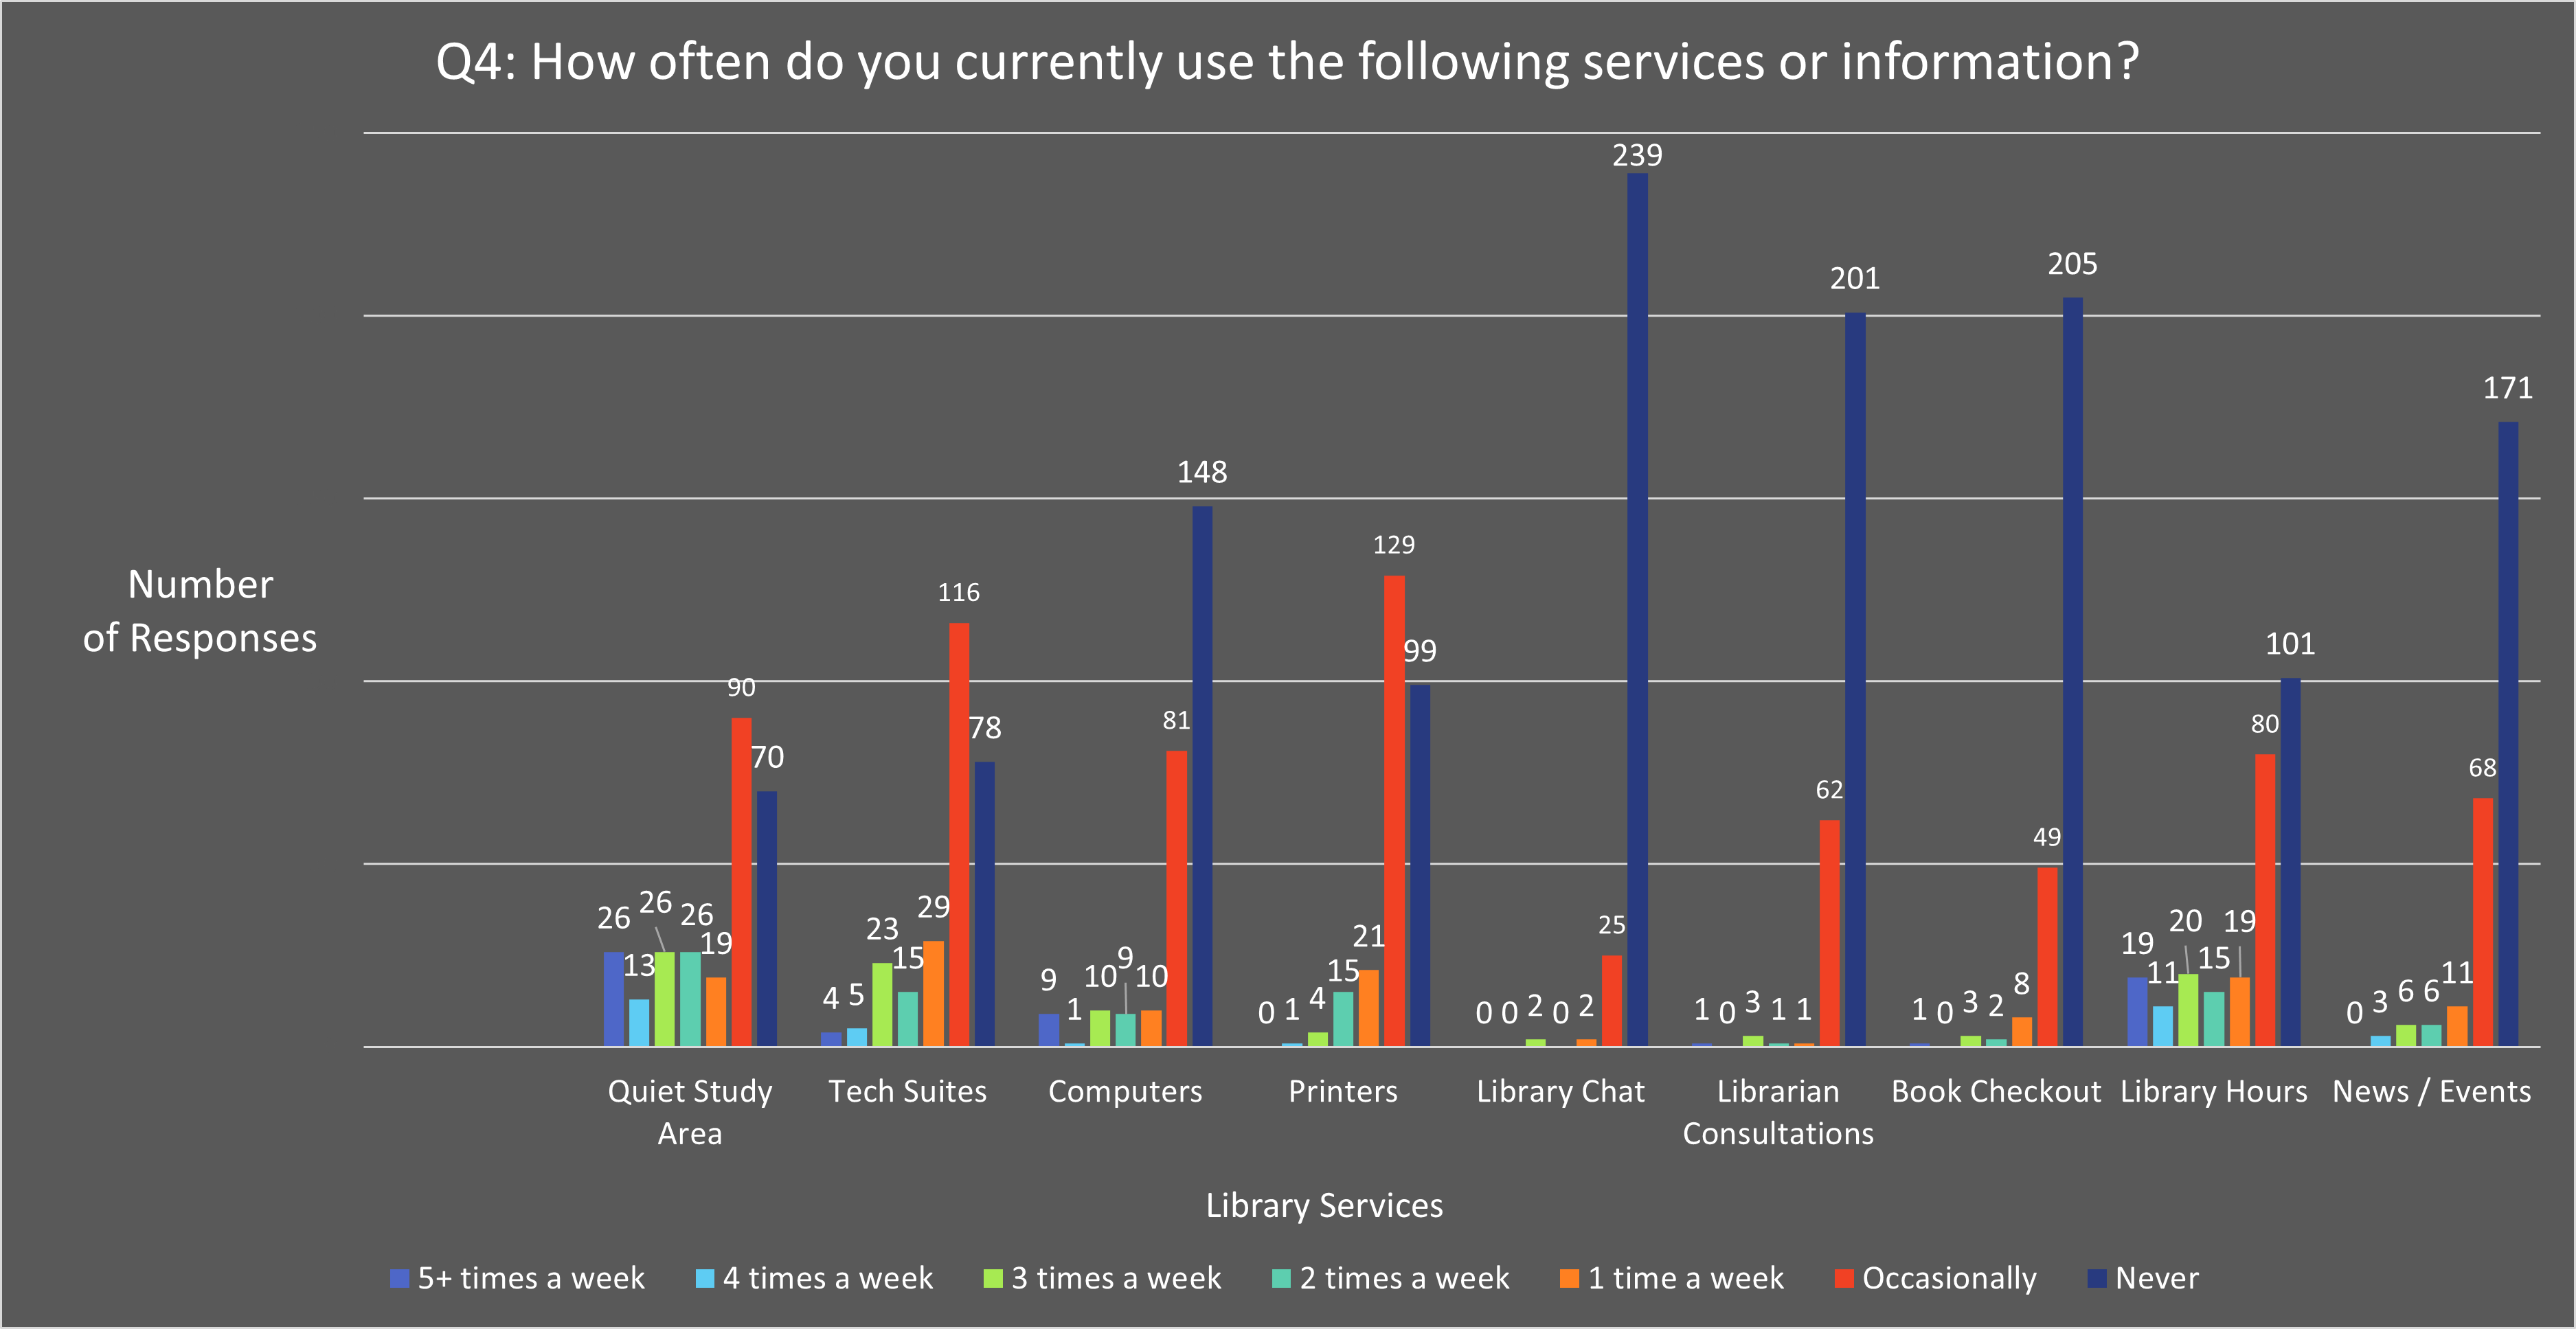
\includegraphics[width = \textwidth, height = \textheight, keepaspectratio]{assets/img/Student Survey Results Q4.png}
         \caption{Current Library Resource Usage}
    \end{figure}

\paragraph{}
In addition to this, the subsequent question in the survey simply asked whether or not the participant would use a mobile library application at all. The majority of responses were either yes or maybe. The corresponding question in the survey (see figure 4.2) provided the respondents with another, similar list of features to consider in the context of a mobile application. This encouraged them to think about which of the proposed features should be included in a mobile app for the Gordon library and which they would realistically use in such a context. This data showed that these features, in theory, would have a greater chance of being used if they were accessible through a mobile app, versus a web page or in-person usage when compared to the previous data in the previous chart.
  \begin{figure}[H]
        \centering
        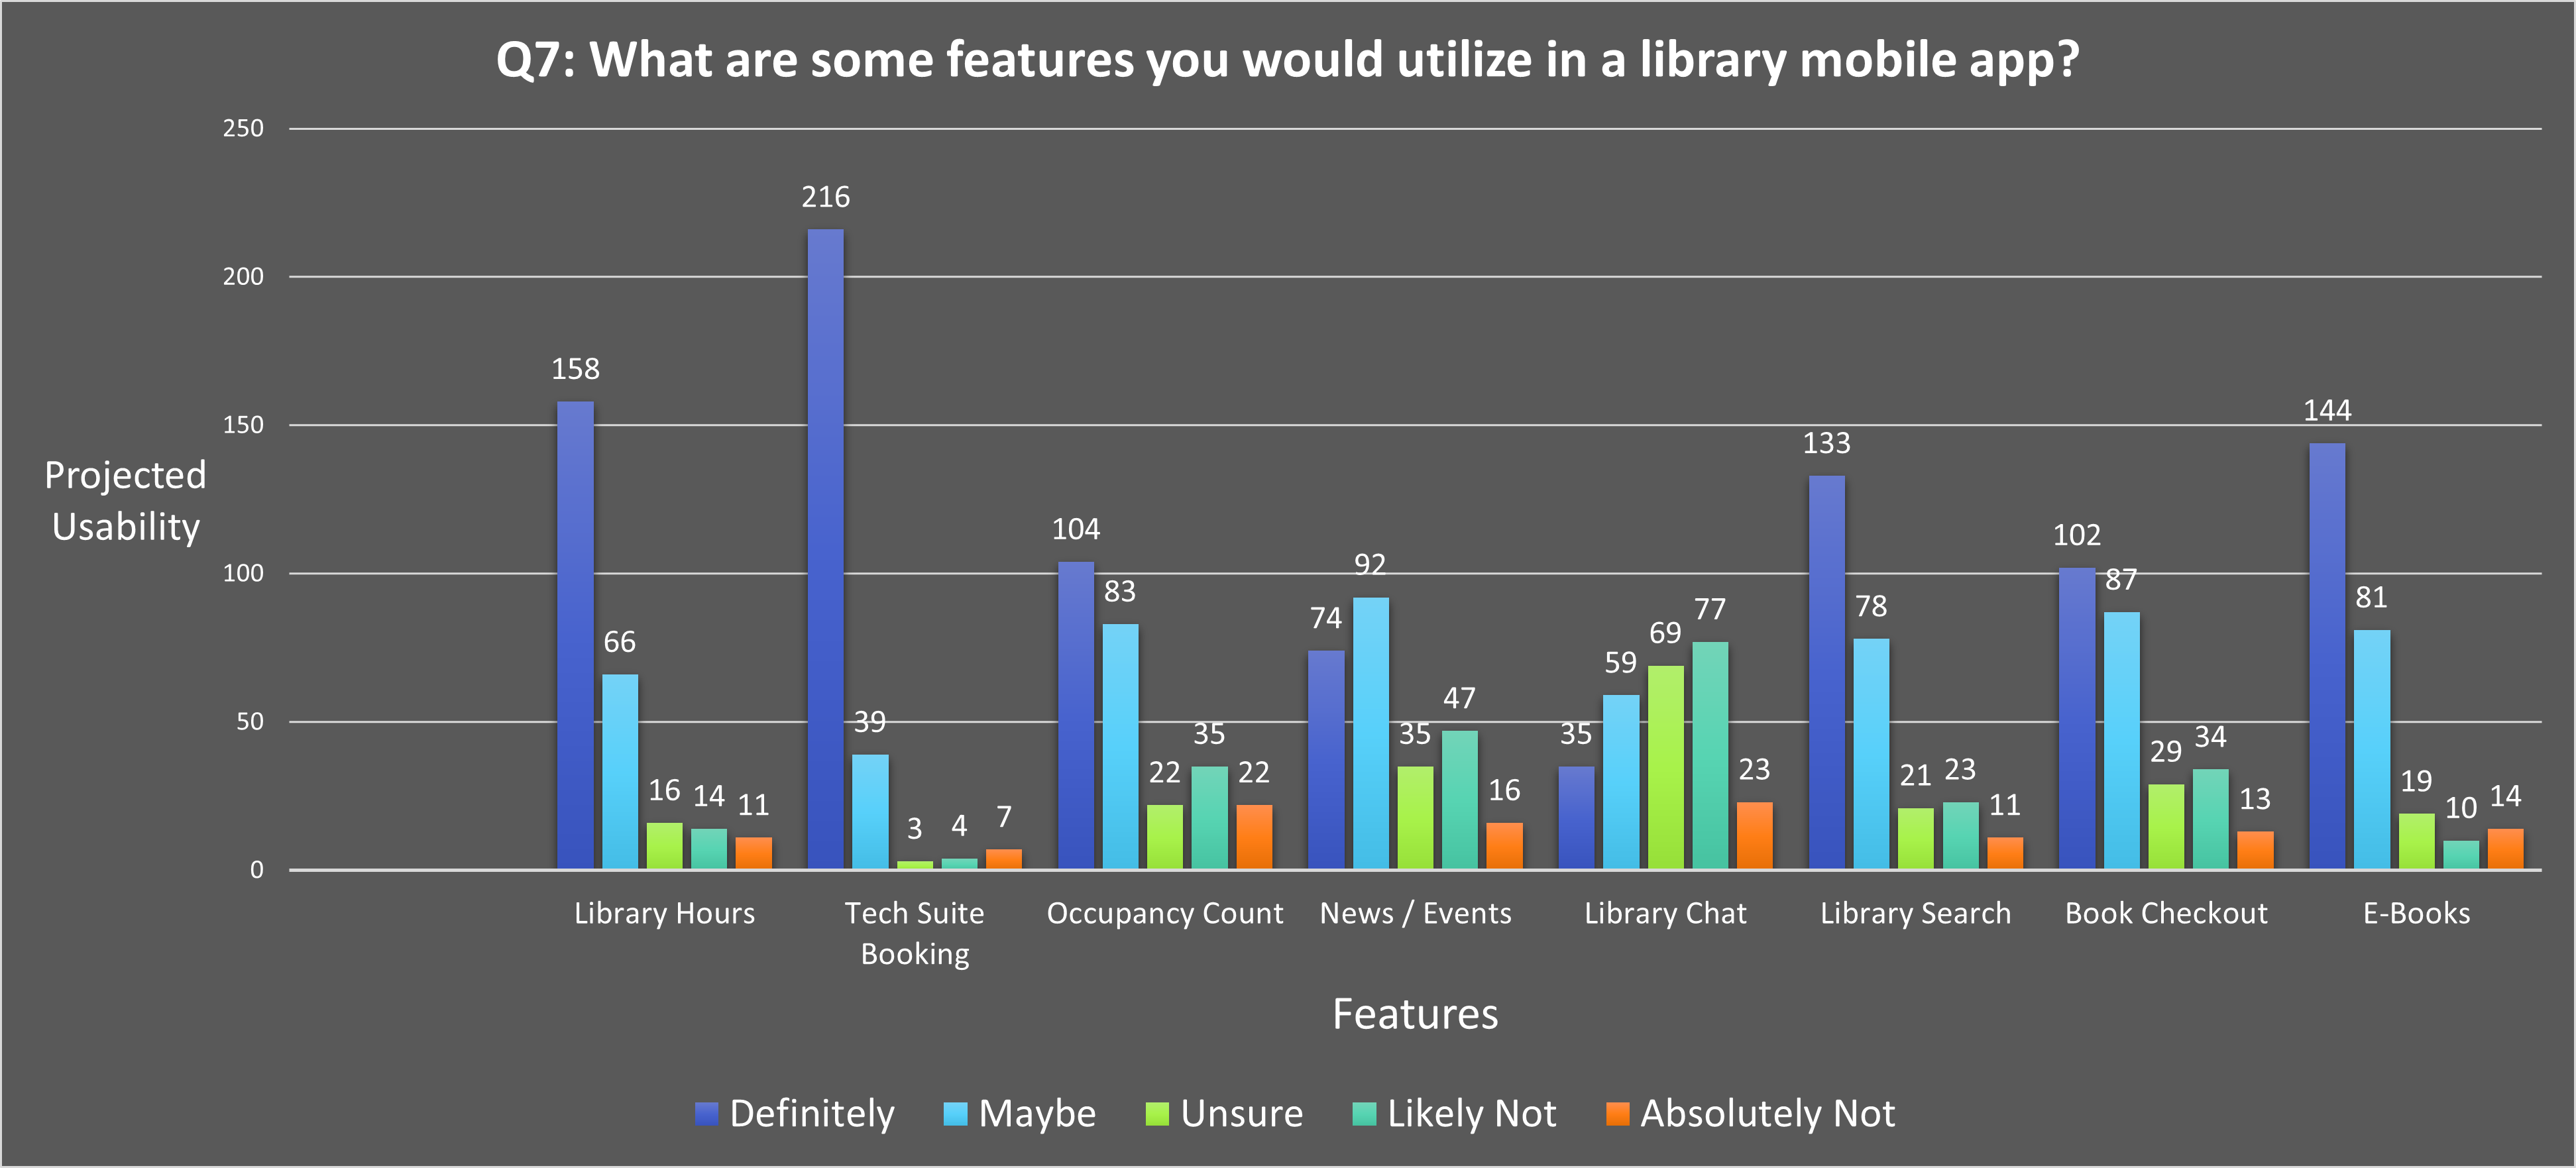
\includegraphics[width = \textwidth, height = \textheight, keepaspectratio]{assets/img/Student Survey Results Q7.png}
        \caption{Features That Might Be Used In A Mobile Environment}
    \end{figure}


\paragraph{}
 This allowed us to then narrow our list of features being considered for implementation to only five: library hours, tech suite booking, occupancy tracking, news and events, and library chat. This list was influenced by both the survey results as shown above, as well as by additional factors regarding the implementation of such features. An example of this was the potential implementation of the library search, book checkout, and e-book features. Each brought steep challenges and were beyond the scope of this project. Therefore, the list was reduced accordingly.
 
\paragraph{}
 Stepping away from the primary features of the mobile app, user interaction and flow had to be considered. Figure 4.3 shows th usage of other non-categorized mobile applications. These apps were chosen simply on the basis of popularity. 
 
 \begin{figure}[H]
        \centering
        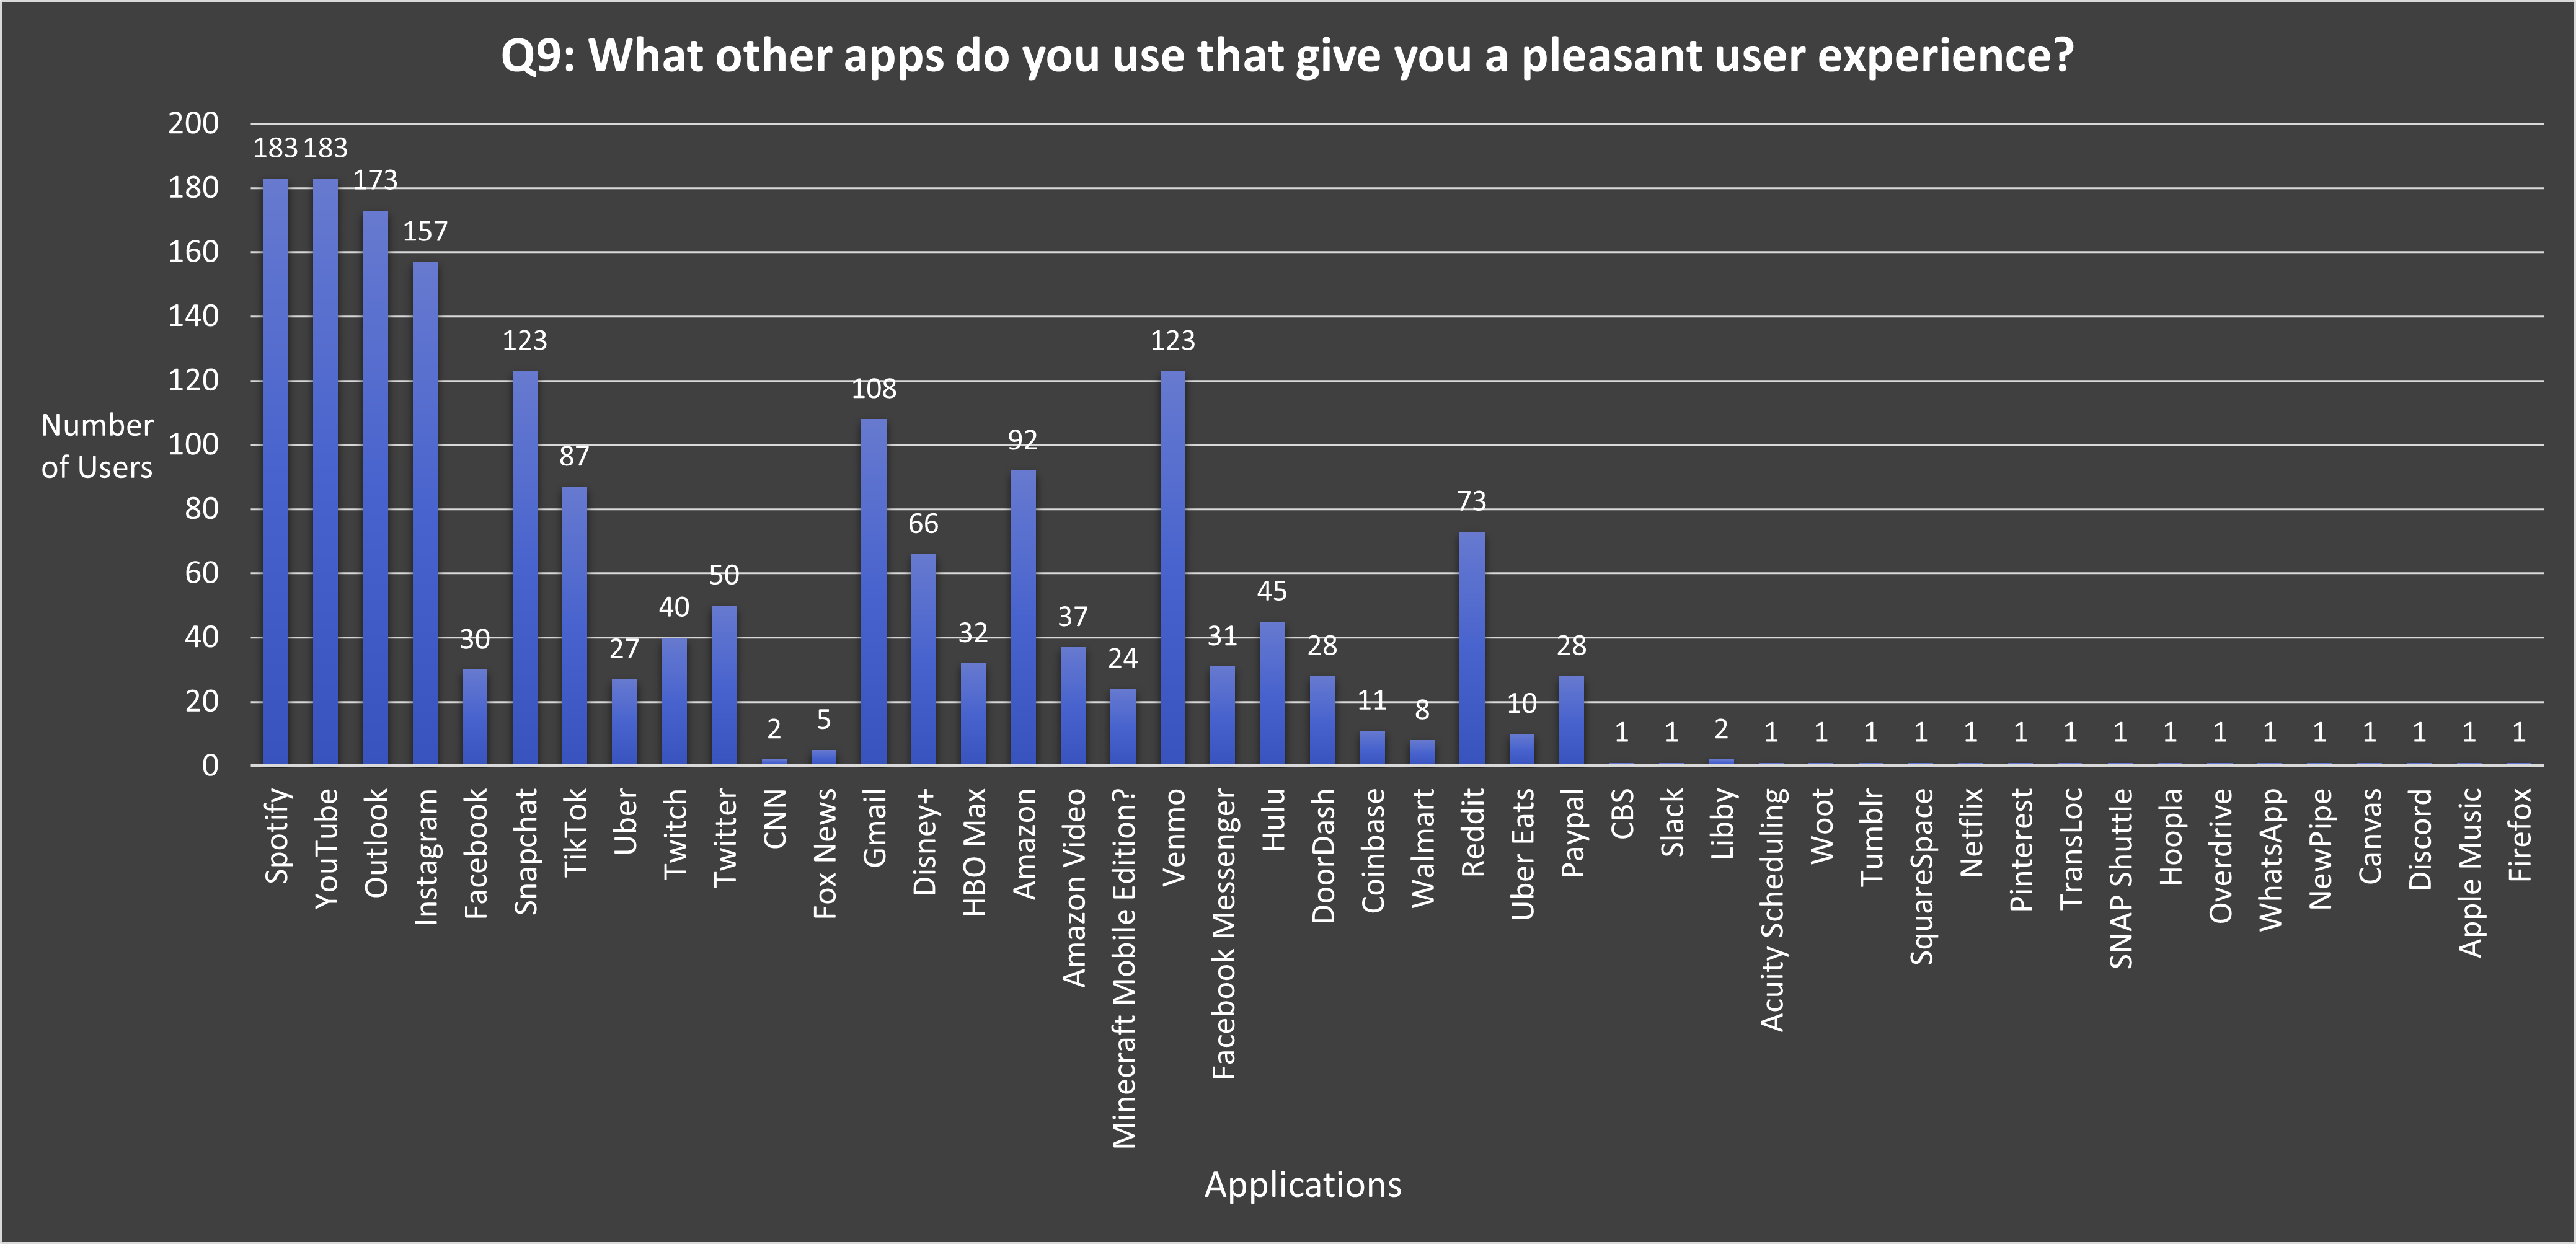
\includegraphics[width = \textwidth, height = \textheight, keepaspectratio]{assets/img/Student Survey Results Q9.png}
         \caption{User Experience Gauge}
    \end{figure}
    
The corresponding survey question allowed the participant to choose as many predetermined apps as they desired, as well as the option to provide additional apps that we did not include. Taking these results into account helped ensure that our application would follow similar modern UI (User Interface) designs like those chosen by the participants in the survey.

\paragraph{}
The final questions the respondents completed in the survey pertained to their willingness to participate as a volunteer tester for the impending prototype. Most respondents, understandably, declined their testing participation, however, 92 individuals chose to participate and 90 of them provided their academic emails for later contact regarding testing our application.

%----------------------------------------------------------------------------------------------------------------------------------------------
\section{Technical}

\paragraph{}
From a technical perspective, progress was made in the design realm. We used Figma to collaborate on these designs. Figma is a online collaborative interface design application. It enabled us to mock-up wireframes in real-time that we would then implement in code later. We began with designing a login page. Our goal was to enable users to only have to log in once, or at least not very often, as it is with various WPI single-sign-on services such as Hub and Canvas. We developed three options as pictured below. There was nothing special about the three designs specifically. We just aimed to offer ourselves some options to implement later. Seeing them helped more than describing them.

% \begin{figure}[h]
%     \centering
%     
\includegraphics[width=0.25\columnwidth]{assets/img/login_1.jpg}
%     \caption{Login Screen Concept \#1}
%     \label{fig:login_1}
% \end{figure}

\begin{figure}[H]
    \centering
    \begin{subfigure}{0.33\textwidth}
        \centering
        
\includegraphics[width=0.6\linewidth]{assets/img/login_1.jpg}
        \caption{Design \#1}
        \label{fig:login_screens_1}
    \end{subfigure}%
    \begin{subfigure}{0.33\textwidth}
        \centering
        
\includegraphics[width=0.6\linewidth]{assets/img/login_2.jpg}
        \caption{Design \#2}
        \label{fig:login_screens_2}
    \end{subfigure}%
    \begin{subfigure}{0.33\textwidth}
        \centering
        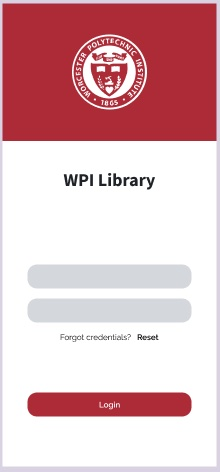
\includegraphics[width=0.6\linewidth]{assets/img/login_3.jpg}
        \caption{Design \#3}
        \label{fig:login_screens_2}
    \end{subfigure}
    \caption{Login Screen Concepts}
    \label{fig:login_screens}
\end{figure}

\paragraph{}
As the planning of the implementation progressed, we decided that a "sign-in" feature would be too cumbersome to implement in the current iteration. We moved on to designing the main page that users would see. Before receiving and reviewing the survey results, we discussed what we would like to see in the app. Considering the pandemic, we knew how important the occupancy count was, so we designed a dedicated page for it. Here are the design concepts we came up with:

\begin{figure}[H]
    \centering
    \begin{subfigure}{0.5\textwidth}
        \centering
        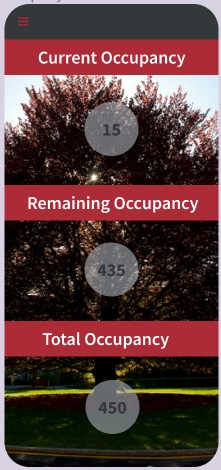
\includegraphics[width=0.6\linewidth]{assets/img/main_1.jpg}
        \caption{Design \#1}
        \label{fig:main_screens_1}
    \end{subfigure}%
    \begin{subfigure}{0.5\textwidth}
        \centering
        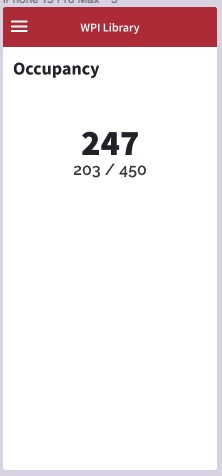
\includegraphics[width=0.6\linewidth]{assets/img/main_2.jpg}
        \caption{Design \#2}
        \label{fig:main_screens_2}
    \end{subfigure}
    \caption{Landing Screen Concepts}
    \label{fig:main_screens}
\end{figure}

\paragraph{}
Neither of these designs satisfied the goals brought forth by the survey results. From our analysis of the survey results, we determined that we would implement something similar to the right figure above, but with more features and functionality. Below the occupancy feature we wanted to embed the library's calendar in a format similar to the WPI website: \url{https://www.wpi.edu/news/calendar?og_group_ref_target_id_entityreference_filter=84091}. Based on the survey results, the feature sought after the most was tech suite booking. So, we planned for a fixed area on the bottom of the page, with a button linking to a page to book a tech suite. "Fixed," meaning that the content remains in place as the user scrolls through the page.

\paragraph{}
After we had determined the look-and-feel according to WPI standards (discussed in our Methodology), we were able to develop a style sheet and suite of reusable components that could have been used in the final product. This was Oliver's doing. He wrote dozens of CSS files and Web Components using the Lit and Vaadin frameworks.

\paragraph{}
Another technical feat was to implement a consumer for the LibCal API. This was completed through the OpenAPI specification. After given access to the LibCal platform at WPI, Oliver was able to write an OpenAPI specification of the API, which would later be used to generate client consumer code. This code would have been used by the mobile app to interact with LibCal's features, specifically so that students could book tech suites directly within the application.



%Furthermore, nearly every aspect of our mobile application was structured by the rubric displayed by modern mobile library applications and student needs to develop the best and most user-friendly application for the George C. Gordon Library and WPI alike. TAKEN FROM RESEARCH


 
%Pages: 14-18

% The Findings or Analysis Chapter: Making 
% Meaning from Your Data 
% The Findings chapter presents what you have found—the key discoveries and/or creations you have made while following your project methodology. It is sometimes called Results and Analysis, or you can give it an even more informational title specific to your project.  
% This chapter is the most important part of your entire project report!  It is where you tell what you learned about the big questions that the previous three chapters set up.   
% To think about what to include in this chapter, it is helpful to make a list of the two or three big questions at the heart of your project.  Think about the goals of the IQP: to examine the relations between science, technology, and society.  What does your project tell us about these relations?  Also, reread your introduction and background.  What is this project all about?   
 
% Content:  This chapter should not be a wholesale information dump of all of your “raw data” organized by technique (e.g., you should not have section headings of “Interview Results”, “Questionnaire Results”, etc.), but rather it should tell the reader what your data mean.  You need to process the data and decide what key findings or patterns have emerged.  In this chapter, your readers will want a SUMMARY of where you ended up and why, not every step along the way. “Analysis” may be a better word than “findings” to describe this chapter. 
% Note that the following would not be a finding: “The average yearly wind speed at the Princeton wind farm is 13.5 mph.” This would be a piece of data. The finding goes deeper and is supported by data. For example, the finding might be, “An expansion of the Princeton wind farm to two 750 kW turbines would pay for itself in eight years.” Some good questions to think about: 
% •	What were your research questions? 
% •	How did different groups of people respond to the situation you are describing? 
% •	What explains why things turned out the way they did? What evidence can you call upon? 
% •	What surprised you about the information you found? How does what you found confirm, contradict, or supplement your sources in the Background chapter?  (Be sure to bring up these sources.)  
% •	Who will be interested in your findings and why?   
% •	What do your findings tell us about the relations between technology and society? 
% It is critically important to weave in discussion about the limitations of your findings—to distinguish between what you can and can’t claim—and to acknowledge alternative interpretations and alternative viewpoints. Although it may seem counterintuitive, your work will seem more credible if you acknowledge limitations and concede some uncertainty.  Your job is not to “sell” any particular results—your job is to help the reader understand how well the results are supported by evidence. 
% A common question, related to interview results in particular, is “What belongs in the Background chapter and what belongs in the Findings chapter?”  It depends, and often there is no clear answer, but you do want to avoid repetition. If the information from the interviews provides additional background information that helps readers understand the problem your project addresses, then you probably want to include it in the Background chapter. This approach is especially common for interviews done in the first week or two of the project that provide context about local issues. However, if the information from your interviews is directly aligned with a research question posed in your Methodology chapter, then that information should be presented as evidence in the Findings chapter 
 
% Structure  
% •	Prepare the reader for your approach by writing an introductory paragraph to the chapter, prior to the first section.  The introduction of this chapter would be an overview of your findings, setting up the rest of the chapter to support those findings.  
% •	Often you can follow the same sequence of objectives or moves that you laid out in the Methodology chapter.  
% •	Depending on your findings and the nature of your project, other organizational strategies might be more effective. For example, in a project that gathers opinions from various stakeholder groups, you could arrange results according to stakeholder group if you want to emphasize those different perspectives, or you could identify themes in the results and then present the views of each stakeholder group within each of those themes.  
% •	An effective format is to state a finding in an introductory paragraph or topic sentence and then support it. It is often tempting to do the reverse, but stating the finding first generally works best for a reader. (See the sample below.) 
% •	Be careful about the amount of detail you provide.  While you should not present all of your raw data, you also need to support your claims; be sure to draw upon your data as evidence for 
% any claims that you make. For example, you could include some quotations from interviews and present summaries of your data in tables or figures.  
% •	Remember that when you include Figures and Tables, you do so to reinforce points you’re making in the narrative, not to replace narrative.  Never present a figure or table unless you refer to it in the text, explain it, and interpret it for the reader. For example: “Table 2 (not ‘The table below’) shows a summary of the results of interviews with the various stakeholder groups, divided into the areas of Strengths, Weaknesses, Opportunities, and Threats. Note that grass-roots contacts and interpersonal connections were a theme among strengths identified by both groups A and B…, whereas …” Then Table 2 should be included in the next available space following this paragraph, and the table should have a fully descriptive caption that is also included in the List of Tables and Figures following the Table of Contents at the front of the report. 
% •	If you are producing some stand-alone documents as part of your work (manual, website, or other materials), plan on placing them in an appendix.  In the Findings chapter, you would describe the findings and principles that guided the development of those documents, and point the reader to them.  The audience for those stand-alone documents is whoever will be using them.  The audience for the report is other researchers. 
 
% Example:  Following is a sample organization for a Findings chapter that illustrates some of the points above.  
% By analyzing the information gathered from our site visits and interviews, we developed the following findings concerning the tree planting projects in Heredia province, and the various stakeholders and principles which affect their success: 
% 1.	Most of the thirteen tree planting sites we visited contained trees that were correctly placed and watered, but were harmed by pests or other isolated incidents Summary of evidence, explanation, and analysis 
% 2.	Tree maintenance programs varied among the sites and the quality of tree maintenance in the private planting sites was superior to the quality of tree maintenance in the public planting sites  Summary of evidence, explanation, and analysis 
% 3.	Participation was low among business owners, developers, and the ordinary community members but was high among community leaders and schools  Summary of evidence, explanation, and analysis 
% 4.	Community members do not participate in their community’s tree planting projects because there is no confidence in the national government’s reforestation efforts, sense of ownership, or opportunity for social interactions  
% Summary of evidence, explanation, and analysis 
% 5.	There were three cases where community members were being empowered, but it appears this is not a widespread occurrence  
% Summary of evidence, explanation, and analysis 

% Features of Effective Conclusions & 
% Recommendations Chapters  
% •	Provide a succinct summary of key findings  
% •	Have directly-stated recommendations that stand out at the beginning of each paragraph or section  
% •	Use formatting that makes it easy for readers to quickly find specific conclusions and recommendations 
% •	Make clear who the recommendations are directed toward 
% •	Show consistency with Background, Methodology, and Findings chapters 
% •	Do more than recommend something; they provide a roadmap for implementation:  What methods?  What criteria should be used? What sources should be consulted? What obstacles might come up? 
            
    \chapter{Conclusion}\addcontentsline{toc}{chapter}{Conclusion}
        

% TODO: The below is from 3.10. See Lori's comments about it.
% "Now that we know that loading is not as easy a we thought, this may just be a plan for what Jimmy could do after approvals, etc."
    The end goal for deployment of this application will be getting it on the mobile app store for android and IOS. This will include confirming the functionality of our app and its compatibility with app store guidelines. Furthermore, this will require submitting a review to the app store to get it approved. The process will require documentation of the app for submission as well as the application itself. It will also require will also have some associated fee. 



% Pages: 6-12


% The Conclusions and Recommendations Chapter 
% Often a reader will want to skim through this final chapter and be able to pick out quickly your specific conclusions and recommendations, so this chapter should be persuasive on its own.  
% Content:  Conclusions can be thought of as a summary of the key findings of your project.  In this sense, it may seem a bit repetitive from your Findings chapter. That’s OK, because sometimes people read only this chapter and not the Findings chapter.  This chapter, however, should be MUCH MORE SUCCINCT.  Instead of giving complete evidence to back up your findings, just suggest the nature of the evidence.  
% Almost all projects will also deliver Recommendations appropriate to your work. Make sure the nature of this chapter is consistent with what you said you would produce in your goal statement.  Generally, very little in this chapter should come as a complete surprise to the reader since findings have already been presented; recommendations should fall out naturally from that discussion.  Note that there are two types of recommendations, those made to address the problem you studied, and those made on next steps of study.  Depending on the nature of your project, you might emphasize recommendations more than conclusions or vice versa. 
% Structure 
% •	As with other chapters, start with a good introductory paragraph.  
% •	Often you can make this chapter more readable by using formatting like bold, italic, or underlining.  You have different options for organizing and formatting this chapter. Sometimes it can be effective to present conclusions and recommendations separately. In other cases, it may work well to present “pairs” of conclusions and recommendations. For example, you could say, 
% “Our results showed that…. In order to address this problem, we recommend that …”  
% •	In a similar manner as the Executive Summary and Findings chapter, make strategic use of formatted lists in this chapter so that readers can easily identify specific conclusions and recommendations. (See example given with Executive Summary.) 
% •	As always, choose your words VERY carefully. A common mistake for recommendations— both in writing and in presentations—is to use statements like “We feel that the Patent and Trademark Office should change its prior art search services by…”  No one should take an action based on how you feel. Rather, you should make clear that your conclusions and recommendations are based on evidence. Therefore, use wording like “We recommend that…” and then accompany that with evidence and justification: “Our results showed that …. Moreover, there was broad support for… Therefore, we conclude…” Keep an objective tone throughout and focus on developing persuasive arguments. Be careful with the word “should.” 
% •	Use active voice, and make clear the audience for each recommendation: “We recommend that Organization X…”  Use words that convey an appropriate level of confidence in your results and recommendations.   
% •	Point out any limitations of your project, and be careful not to make the scope of your claims more broad than is justified by your results. Your argument will be more persuasive if you acknowledge limitations and alternatives you considered. 
% •	Often it is difficult to figure out how to conclude this chapter, and a concept that may be helpful is to think of it as an inverse funnel. The whole report up to that point has been funneling down to the specific findings and the accomplishment of your goal, but then you want to funnel back out and point out things like the long-term implications of your work, who will benefit from your work, possible uses of your findings and recommendations by individuals or groups other than your project sponsor, and/or interesting questions that your work raises that could be pursued by others in the future. You’d like the reader to be thinking “WOW!” at the end of this chapter, which you can only accomplish with meaningful rather than superficial concluding remarks. 
 
 
% The Abstract 
% The Abstract is one of the last portions of your project to be written.  It should mention the sponsor if you have one, describe the problem and goal of the project, perhaps give an overview of the methods, and give a sense of the nature of the findings, conclusions, and recommendations. It needs to fit in the space on the CDR form; this is described as 80 words, but generally a bit more than that can fit in. Typically that’s 4-6 sentences: perhaps one describing the problem, one stating your goal, one giving a sense of the methods, and two or so suggesting the nature of conclusions and/or recommendations. Your IQP abstract will appear on your WPI transcript, so try to convey the significance of your work, and make clear if it was completed for an external organization. 
            
    \chapter{Recommendations}\addcontentsline{toc}{chapter}{Recommendations}
        % Pages: 6-12


% The Conclusions and Recommendations Chapter 
% Often a reader will want to skim through this final chapter and be able to pick out quickly your specific conclusions and recommendations, so this chapter should be persuasive on its own.  
% Content:  Conclusions can be thought of as a summary of the key findings of your project.  In this sense, it may seem a bit repetitive from your Findings chapter. That’s OK, because sometimes people read only this chapter and not the Findings chapter.  This chapter, however, should be MUCH MORE SUCCINCT.  Instead of giving complete evidence to back up your findings, just suggest the nature of the evidence.  
% Almost all projects will also deliver Recommendations appropriate to your work. Make sure the nature of this chapter is consistent with what you said you would produce in your goal statement.  Generally, very little in this chapter should come as a complete surprise to the reader since findings have already been presented; recommendations should fall out naturally from that discussion.  Note that there are two types of recommendations, those made to address the problem you studied, and those made on next steps of study.  Depending on the nature of your project, you might emphasize recommendations more than conclusions or vice versa. 
% Structure 
% •	As with other chapters, start with a good introductory paragraph.  
% •	Often you can make this chapter more readable by using formatting like bold, italic, or underlining.  You have different options for organizing and formatting this chapter. Sometimes it can be effective to present conclusions and recommendations separately. In other cases, it may work well to present “pairs” of conclusions and recommendations. For example, you could say, 
% “Our results showed that…. In order to address this problem, we recommend that …”  
% •	In a similar manner as the Executive Summary and Findings chapter, make strategic use of formatted lists in this chapter so that readers can easily identify specific conclusions and recommendations. (See example given with Executive Summary.) 
% •	As always, choose your words VERY carefully. A common mistake for recommendations— both in writing and in presentations—is to use statements like “We feel that the Patent and Trademark Office should change its prior art search services by…”  No one should take an action based on how you feel. Rather, you should make clear that your conclusions and recommendations are based on evidence. Therefore, use wording like “We recommend that…” and then accompany that with evidence and justification: “Our results showed that …. Moreover, there was broad support for… Therefore, we conclude…” Keep an objective tone throughout and focus on developing persuasive arguments. Be careful with the word “should.” 
% •	Use active voice, and make clear the audience for each recommendation: “We recommend that Organization X…”  Use words that convey an appropriate level of confidence in your results and recommendations.   
% •	Point out any limitations of your project, and be careful not to make the scope of your claims more broad than is justified by your results. Your argument will be more persuasive if you acknowledge limitations and alternatives you considered. 
% •	Often it is difficult to figure out how to conclude this chapter, and a concept that may be helpful is to think of it as an inverse funnel. The whole report up to that point has been funneling down to the specific findings and the accomplishment of your goal, but then you want to funnel back out and point out things like the long-term implications of your work, who will benefit from your work, possible uses of your findings and recommendations by individuals or groups other than your project sponsor, and/or interesting questions that your work raises that could be pursued by others in the future. You’d like the reader to be thinking “WOW!” at the end of this chapter, which you can only accomplish with meaningful rather than superficial concluding remarks. 



\section{Development Approach}

\paragraph{}
To be clear, this section discusses the entirety of the development from preliminary


\section{Techniques for Deployment}

% TODO: Rewrite (from 3.10):
\paragraph{}
The end goal was to deploy the final application on mobile app stores: iOS and Android. When we began development, we shifted our approx from writing a native application to a web applica- tion. This choice removed the possibility of deployment to the the iOS app store, but seemed the most logical route to complete to project in time. Deployment was never achieved, and thus our recommendations to continue the project are discussed in our conclusion.
    
    %  \settocbibname{References}
    % \bibliographystyle{apacite}
    % \bibliography{references}
    \chapter{Bibliography}\addcontentsline{toc}{chapter}{Bibliography}
        
\section{References}

\paragraph{}Anand, A., Kaur, J. & Inoue, S. (2020). Reliability modeling of multi-version software system incorporating the impact of infected patching. \textit{International Journal of Quality & Reliability Management,} 37(6/7), 1071-1085. https://doi.org/10.1108/IJQRM-07-2019-0247 


\paragraph{}
Behrang, F., & Orso, A. (2018, May). Automated test migration for mobile apps. ICSE '18: 40th International Conference on Software Engineering, Gothenburg, Sweden. https://doi.org/10.1145/3183440.3195019 

\paragraph{}
Chen, S.-c. (2019). Undergraduate students use of mobile apps to search library catalogs. \textit{Library Hi Tech,} 37(4), 721-734. https://doi.org/10.1108/LHT-12-2018-0198 

\paragraph{}
Ex Libris. (2017, October 31). \textit{Ex Libris campusM mobile app now enhancing student engagement at 50 UK campuses} [Press release]. https://exlibrisgroup.com/press-release/ex-libris-campusm-mobile-app-now-enhancing-student-engagement-at-50-uk-campuses/

\paragraph{}
Hu, Y., & Neamtiu, I. (2016, May). \textit{Fuzzy and cross-app replay for smartphone apps}. AST ’16: 11th International Workshop on Automation of Software Test, Austin, Texas. https://doi.org/10.1145/2896921.2896925

\paragraph{}
Huy, N. P., & vanThanh, D. (2012, December). \textit{Evaluation of mobile app paradigms}. MoMM '12: 10th International Conference on Advances in Mobile Computing & Multimedia, Bali, Indonesia. https://doi.org/10.1145/2428955.2428968

\paragraph{}
Mansouri, A., & Soleymani Asl, N. (2019). Assessing mobile application components in providing library services. \textit{The Electronic Library}, 37(1), 49-66. https://doi.org/10.1108/EL-10-2018-0204

\paragraph{}
Margam, M., & Saleeq,  A. D. (2017). Mobile information services and initiatives in university libraries: A new way of delivering information. \textit{Journal of Library & Information Technology}, 37(2), 109-118. https://doi.org/ 10.14429/djlit.37.2.11116

\paragraph{}
MobiOne Developer 1.0 M4: Create app store-ready mobile web applications, experience true device behavior on Windows. (2009, October 2). \textit{Genuitec}. https://www.genuitec.com/mobione-developer-1-0-m4-create-app-store-ready-mobile-web-applications-experience-true-device-behavior-on-windows/

\paragraph{}
Nagappan, M., Shihab, E., & Hassan, A. E. (2013, November 18-20). \textit{Challenges in mobile apps: A multi-disciplinary perspective}. CASCON '13: 2013 Conference of the Center for Advanced Studies on Collaborative Research, Ontario, Canada. https://doi.org/ 10.5555/2555523.2555578

\paragraph{}
New York University. (2021, April 5). \textit{NYU pilot program offers students and faculty instant access to 150,000 ebooks via app} [Press Release]. https://www.nyu.edu/about/news-publications/news/2021/april/pilot-program-offers-nyu-students-and-faculty-instant-access-to-.html

\paragraph{}
Pu, Y.-H., Chiu, P.-S., Chen, T.-S., & Huang, Y.-M. (2015). The design and implementation of a Mobile Library APP system. \textit{Library Hi Tech}, 33(1), 15-31. https://doi.org/10.1108/LHT-10-2014-0100

\paragraph{}
Quispe, B. M., Casas, L. A., Oviedo, O. A., Quispe, J. H., Chavez, C. V., Pucho, R. V., Choquehuayta, A., & Joaquín, B. D. (2018, October). \textit{Influence of the use of educational apps on smart mobile devices in the academic performance of students}. ICETC '18:10th International Conference on Education Technology and Computers, Tokyo, Japan. https://doi.org/10.1145/3290511.3290541

\paragraph{}
Sadeghi, A., Esfahani, N., & Malek, S. (2017, September). \textit{Mining mobile app markets for prioritization of security assessment effort}. WAMA 2017: 2nd ACM SIGSOFT International Workshop on App Market Analytics, Paderborn, Germany. https://doi.org/10.1145/3121264.3121265

\paragraph{}
Saragossi, J., Costello, L., & Kasten, K.   (2018).   Mobile applications in academic libraries. Library Resources & Technical Services, 62(4), 198-204. https://doi.org/10.5860/lrts.62n4.198

\paragraph{}
Shahriza Abdul Karim, N., Hawa Darus, S., & Hussin, R. (2006). Mobile phone applications in academic library services: A students' feedback survey. \textit{Campus-Wide Information Systems}, 23(1), 35-51. https://doi.org/10.1108/10650740610639723 

\paragraph{}
Wang, H., Liu, Z., Guo, Y., Chen, X., Zhang, M., Xu, G., & Hong, J. (2017, April). \textit{An explorative study of the mobile app ecosystem from app developers' perspective}. WWW '17: 26th International Conference on World Wide Web, Perth, Australia. https://doi.org/10.1145/3038912.3052712

\paragraph{}
Yip, K. H. T., Lo, P., Ho, K. K. W., & Chiu, D. K. W. (2021). Adoption of mobile library apps as learning tools in higher education: A tale between Hong Kong and Japan.\textit{Online Information Review}, 45(2), 389-405. https://doi.org/10.1108/OIR-07-2020-0287 
    
    
    \chapter{Appendix}\addcontentsline{toc}{chapter}{Appendix}
        \section{Timeline}\addcontentsline{toc}{section}{Timeline}
        \paragraph{}
Our timeline (Figure~\ref{fig:project_timeline}), named \textit{Muirhead-Scanlon-Yasuna Chart}, depicts a similar setup to the popular Gantt Chart, however, it is not the same. It could be considered a derivative of a stripped-down Gantt Chart. Like a Gantt Chart, the $x$-axis expresses time and the $y$-axis lists tasks. In our particular case, time is divided into three sections, one for each WPI term. Under these sections, there exists a subsection for each week of the term. The lowest unit of measurement displays the week of the term, listed as Sunday through Saturday. This chart aided in the team's productivity, keeping each member responsible for their individual efforts, as well as, allowing us to keep track of our deadlines.


\begin{figure}[H]
    \hspace*{-2.25cm}
    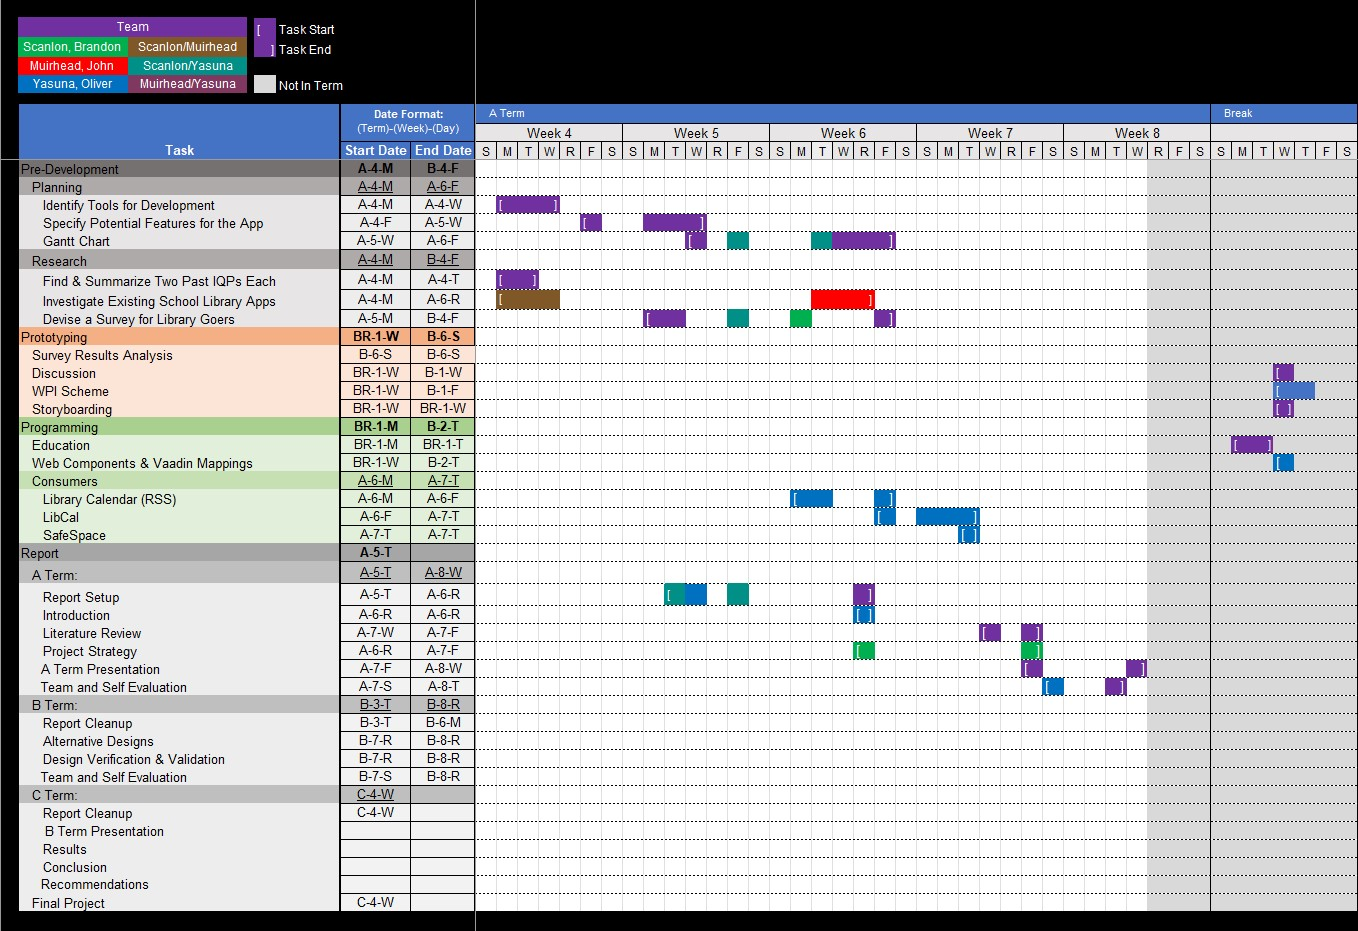
\includegraphics[scale=.58]{assets/img/Term A Timeline.jpg}
    \caption{Term A Project Timeline}
    \label{fig:project_timeline}
\end{figure}

\begin{figure}[H]
 \hspace*{-2.25cm}
    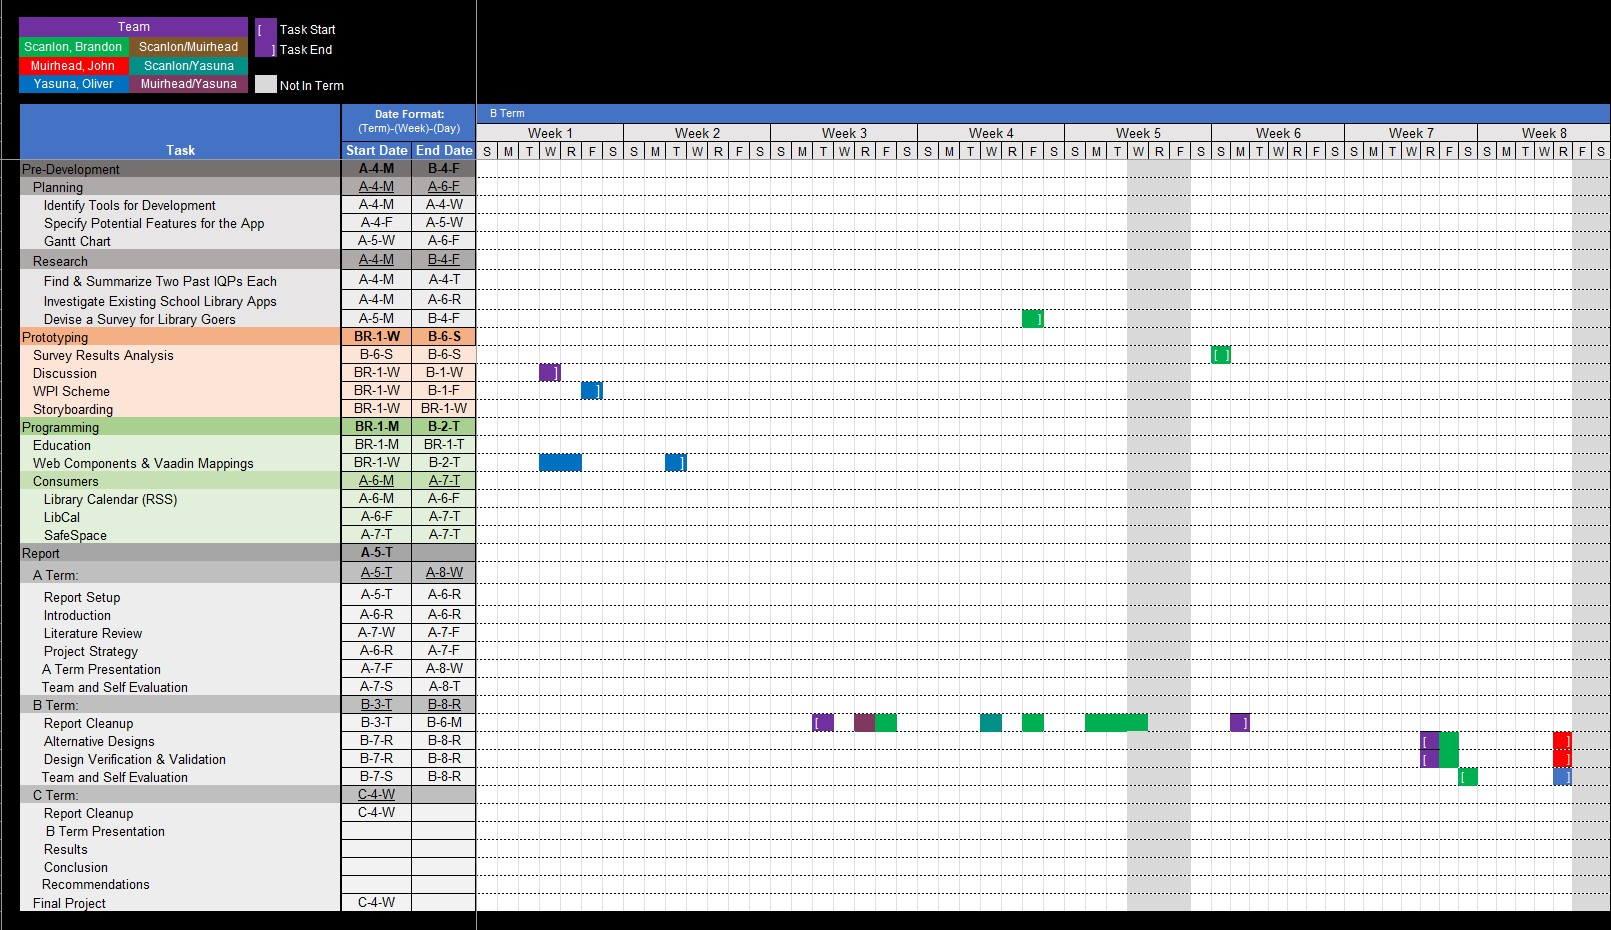
\includegraphics[scale=.49]{assets/img/Term B Timeline.jpg}
    \caption{Term B Project Timeline}
    \label{project_timeline}
\end{figure}

        \section{Additional Mobile Academic Library App Research}
        \subsection{Harvard and Bennett University}
            \paragraph{}
            Harvard and Bennet university had simnular app designs. Harvard's library app, Harvard Library, featured a minimalist home screen with the school logo in the upper-right hand corner, a help button in the lower-left, a 'login' feature in the lower right, and a circular 'start' button in the center. The screen featured only three colors; white, black and crimson red. Clicking the 'start' button pulled up the same login screen that clicking the 'login' button pulled up.  Unfortunately, we were not able to further explore this mobile app because we do not have account affiliated with the University. The home screen for this application can be seen in the following image: 
            \begin{figure}[htbp]
            \centerline{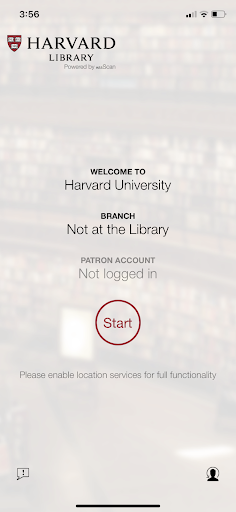
\includegraphics[width=2.5in]{unnamed-4.png}}
            \end{figure}
            The Bennet University app was similar in that unless you had an account, you could not log in and work with it at all. This application had less slick of a design. Some application developers, seem to value exclusivity and privacy. 
        \subsection{Salisbury}
            \paragraph{}
            Sailsbury Universitie's Library app, SU Libraries, featured a noticeably less minimalist design than Harvard's, and had a more unrefined look.  Fortunately, we were able to access the applications features. The home screen included a search bar, and nine features: "Library Hours", "Research Help", "Room Reservations", "Self Checkout", "SU Libraries MakerLab", "Device Availability", "Building Maps", "Helpful Links" and "Contact Information". It also contained a bar at the bottom with five navigation options: "Home", "Library News", "Chat", "My Card" and "About". Additionally, there was a link to the libraries social media accounts. The home screen of this application can be seen in the following image: 
            \begin{figure}[htbp]
            \centerline{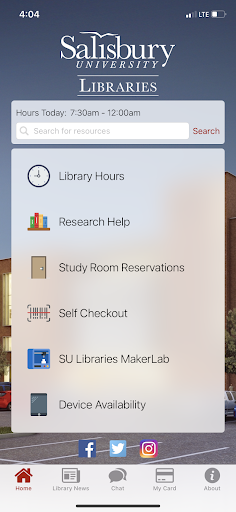
\includegraphics[width=2.5in]{unnamed-3.png}}
            \end{figure}
            \paragraph{}
            The "Library Hours" feature lead to a screen with minimal interactivity. The screen contained the opening and closing times for all days from the current day to approximately three months in advance. The "Research Help" feature took the user to a page with a somewhat similar layout; a page in which you could scroll downward, containing the subjects in which you could get research help. This page, however, was interactive. The user could click on each subject option, taking them to a page with information about who to contact, and how to contact them, if they are seeking research help in that specific area.  The "Study Room Reservations" feature as well as the "Devise Availability" feature has a similar layout to these two.
            \paragraph{}
            The "Building Maps" feature lead to a page containing the layout of each floor of the building. The only interactivity on this page was the option to click on any of the diagrams for an enlarged view of the diagram. 
            \paragraph{}
            The "SU Libraries MakerLab" feature took the user to a page which seemed to function like an app in and of itself. The page it took the user to contained a variety of features relating to the Maker Lab. Such as a feature displaying the time it's open for today as well as a feature displaying which days it is open. It also had a feature taking the user to a page with the Maker Lab policies, a feature allowing users to make an appointment in the maker space, and finally the contact information for the maker space.
        \subsection{University Of Dallas}
            \paragraph{}
            The University of Dallas app had a simple white, black, and Navy blue design. The app consisted of a home screen with four main sections. These sections were "Nearest Libraries", "My Account", "eBooks & eAudio", and "Social". The application also featured a search bar. All of the apps analyzed so far make use of a search functionality. The home screen of this application can be seen in the following image: 
            \begin{figure}[htbp]
            \centerline{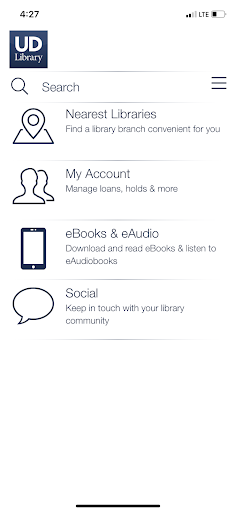
\includegraphics[width=2.5in]{unnamed-2.png}}
            \end{figure}
            \paragraph{}
            \paragraph{}
            Furthermore, like the Harvard app but unlike the Sailsbury app, this app featured a login option. The eBooks & eAudio section linked to a bar code scanner. I think it would be fair to assume this functionality relates to some specific feature at the university of Dallas library. The social tab lead to a link to the libraries social media, namely Facebook, Instagram and Twitter. This seems like a relatively easy functionality to implement, yet still very important. 
        \subsection{University of Sydney}
            \paragraph{}
            This application featured a black white and Orange user interface. The application featured an abundant amount of functions and utilities at the users disposal. These included, but were not limited to: "Libraries", "Book a Study space", "News-Events", "Services", "Scab ISBN" and more. Furthermore, each section had many subsections within it. For example, "Services" encompassed "Study", "Research", "Appointments", and "Disability". They also did indeed contain a section for social media as well as a search bar. The university of Sydney created an extensive application filled with various functionality and features. While the application may seem unwieldy at first, upon familiarizing oneself with the app, it has potential to offer great utility.  
            The home screen of this application can be seen in the following image: 
            \begin{figure}[htbp]
            \centerline{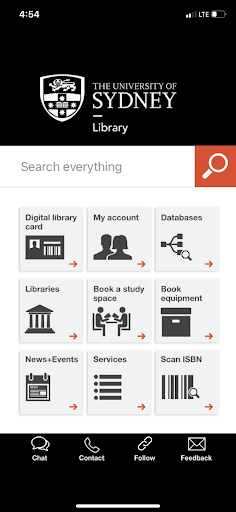
\includegraphics[width=2.5in]{unnamed.png}}
            \end{figure}
            \paragraph{}
        \subsection{Cairn, Parket, Ajman}
            \paragraph{}
            Three other apps which we explored which had a very similar design were that of Cairn University, Parket university, and Ajman University. Each of them had two, potentially three, features. A search with a bar at the top. Presumably, only books could be searched for, but there was also an option to scan books. Below that, two of the apps, Cairn and Parket, featured a scroll bar of book covers at the bottom. These three apps seemed almost identical to one another in style and functionality. 
            
            
        \subsection{Similarities}
        We noticed some similarities among the  applications we analyzed. Firstly, the layout for most of them was the same; a home screen which contained a variety of possible features that, when clicked, would lead to another screen or a pop-up further elaborating on that feature. Some of the specific features were common among many of the applications. For example, four of the eight apps had a functionality for logging in. While this may offer some benefits to the user, it seems difficult to implement and only necessary if you have already implemented some other specific features, such as book checkout. Another feature available in two of the eight apps was a link to the social media; this feature has great utility and would be easy to implement. Finally, there were obvious similarities between the Cairn, Parket, and Ajman apps. They all had the exact same format.
    
        \section{Academic Library Features}

    \noindent{} The following is based from the research gathered by a study conducted by Mansouri and  Soleymani in 2018. Each resource was considered based on the capabilities they provide and if they fit within the demographic of our mobile library application..
    
    \paragraph{Search (by barcode/QR code scan)}
    We assumed these features refer to a user's ability to search the library catalog. We decided to not implement this feature in the \appname app. However, it is an important one, as according to this study, all existing library apps reviewed had this feature. We believe for a mobile app that is intended to be a replacement for a desktop website to be successful, it must provide the most common services provided by its desktop website counterpart.
    
    \paragraph{Tutorial}
    We assume this feature refers to a visual tutorial provided within the mobile app that teaches new users how to use said mobile app. The study found that 70\% of library mobile apps had this feature. A tutorial allows new users to get a better understanding of how to use a platform. Without a tutorial, many new users may be lost, therefore rendering the mobile app useless for them. Although we considered adding a tutorial feature to our app, it was not included in our final design.
    
    \paragraph{Ask a librarian}
    We assumed this feature refers to a user's ability to submit questions to a librarian. The study found all library mobile apps included this feature. Our design plans included a similar feature: the library chat.
    
    \paragraph{Hours}
    Straight-forward features that provides users with library hours. This feature is part of the \appname app design plan.
    
    \paragraph{Events}
    We assumed this feature refers to a user's ability to view library events and/or a calendar. The study found that 90\% of library mobile apps have this feature. Implementation of this feature is in our design plan. Users should not have to use a separate service.
    
    \paragraph{FAQ/Feedback}
    It surprised us that only 30\% of library mobile apps have this feature. The whole point of a library application is to provide students easier access to the WPI library's various services. It is impossible to make a perfect product, because there is always some disconnect between what the developers think consumers want, and what the consumers actually want. The design plan includes a platform for users of the \appname app to provide feedback on their experience.
        \section{Student Survey}

\paragraph{}
\noindent\textbf{WPI George C. Gordon Library Mobile App}
\newline
\noindent Our IQP team is investigating the development of a mobile library app. We are seeking your feedback on the potential resources and services WPI users would utilize in this app.
All responses to the survey are completely anonymous, and cannot be traced back to the respondent. You may however, provide your WPI email address at the end, and we may contact you to discuss additional ideas. 
If you have any questions or concerns about this survey or project, please choose to contact us at:
gr-libappteam@wpi.edu
*All of the following questions and the entire survey are both completely optional*
\newline


\noindent\textbf{Question 1: What is your current academic status at WPI?}
\begin{itemize}
    \item Certificate
    \item Undergraduate
    \item Master's
    \item PhD
    \item Other:
\end{itemize}
\newline


\noindent\textbf{Question 2: What is your declared major?}
\paragraph{}
Choose
\newline


\noindent\textbf{Question 3: What is your current enrollment status?}
\begin{itemize}
    \item Full-time
    \item Part-time
    \item Not currently enrolled
\end{itemize}
\newline


\noindent\textbf{Question 4: How often do you currently use the following services or information?}
\begin{figure}[H]
    \centering
     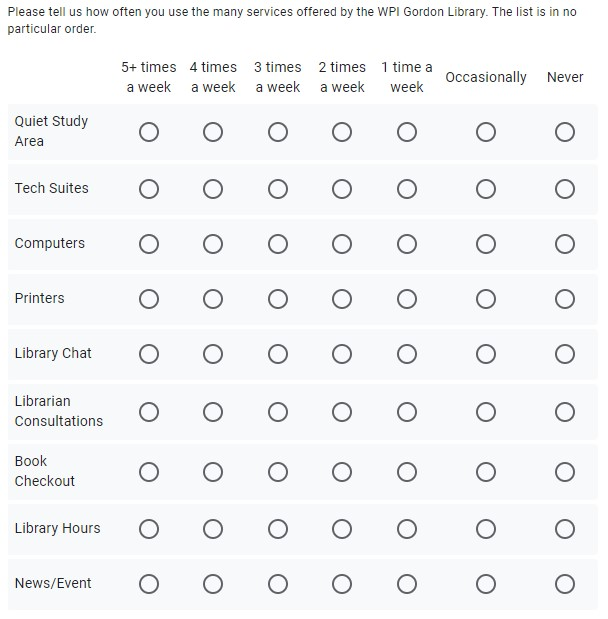
\includegraphics[width = \textwidth, height = \textheight, keepaspectratio]{assets/img/Initial Survey Q4.jpg}
\end{figure}
\newline


\noindent\textbf{Question 5: Would you use a mobile app for the WPI Gordon Library?}
\begin{itemize}
    \item Yes
    \item No
    \item Maybe
\end{itemize}
\newline


\noindent\textbf{Question 6: If answered "no" to the previous question, please explain why.}
\paragraph{}
Your answer
\newline


\noindent\textbf{Question 7: What are some features you would utilize in a library mobile app?}
\begin{figure}[H]
    \centering
     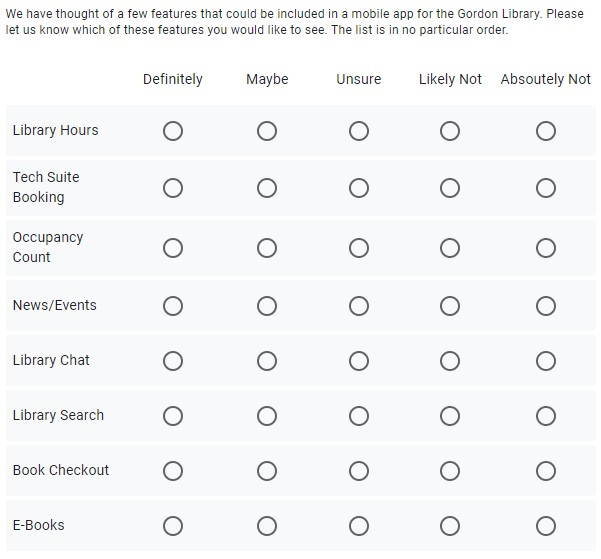
\includegraphics[width = \textwidth, height = \textheight, keepaspectratio]{assets/img/Initial Survey Q7.jpg}
\end{figure}
\newline


\noindent\textbf{Question 8: Do you suggest any additional features not shown above?}
\paragraph{}
Your answer
\newline


\noindent\textbf{Question 9: What other apps do you use that give you a pleasant user experience?}
\newline
To provide the highest quality mobile app for our library, please let us know what apps you enjoy using to use as references.
\begin{itemize}
    \item Spotify
    \item YouTube
    \item Outlook
    \item Instagram
    \item Facebook
    \item Snapchat
    \item Tiktok
    \item Uber
    \item Twitch
    \item Twitter
    \item CNN
    \item Fox News
    \item Gmail
    \item Disney+
    \item HBO Max
    \item Amazon
    \item Amazon Video
    \item Minecraft Mobile Edition?
    \item Venmo
    \item Facebook Messenger
    \item Hulu
    \item DoorDash
    \item Coinbase
    \item Walmart
    \item Reddit
    \item Uber Eats
    \item Paypal
    \item CBS
    \item Other:
\end{itemize}
\newline


\noindent\textbf{Question 10: Would you be willing to participate as a volunteer to test our mobile library app over the next two terms? If so, please provide us with your WPI email in the next section.}
\newline
As we progress in the development of this mobile library app, we will be requiring a test group willing to volunteer and test the various stages of our app.
\begin{itemize}
    \item Yes
    \item No
\end{itemize}
\newline


\noindent\textbf{Question 11: Please provide your WPI email (optional) if you would like for us to contact you.}
\newline
This is completely optional and you may choose to remain anonymous for the survey. Otherwise, please use your WPI email.
\newline


\noindent\textbf{Question 12: Do you have any additional comments about the development of this library app?}
\paragraph{}
Your answer
        \section{Student Survey Results}

\paragraph{}

The student survey was conducted in the beginning of November 2021 using Google Forms. Twelve optional questions were included. A total of 271 responses were collected and analyzed between November 28 and December 10.

\paragraph{}
%------------------------------------------------------------------------------------------------------------------------------------------
 \begin{figure}[H]
        \centering
        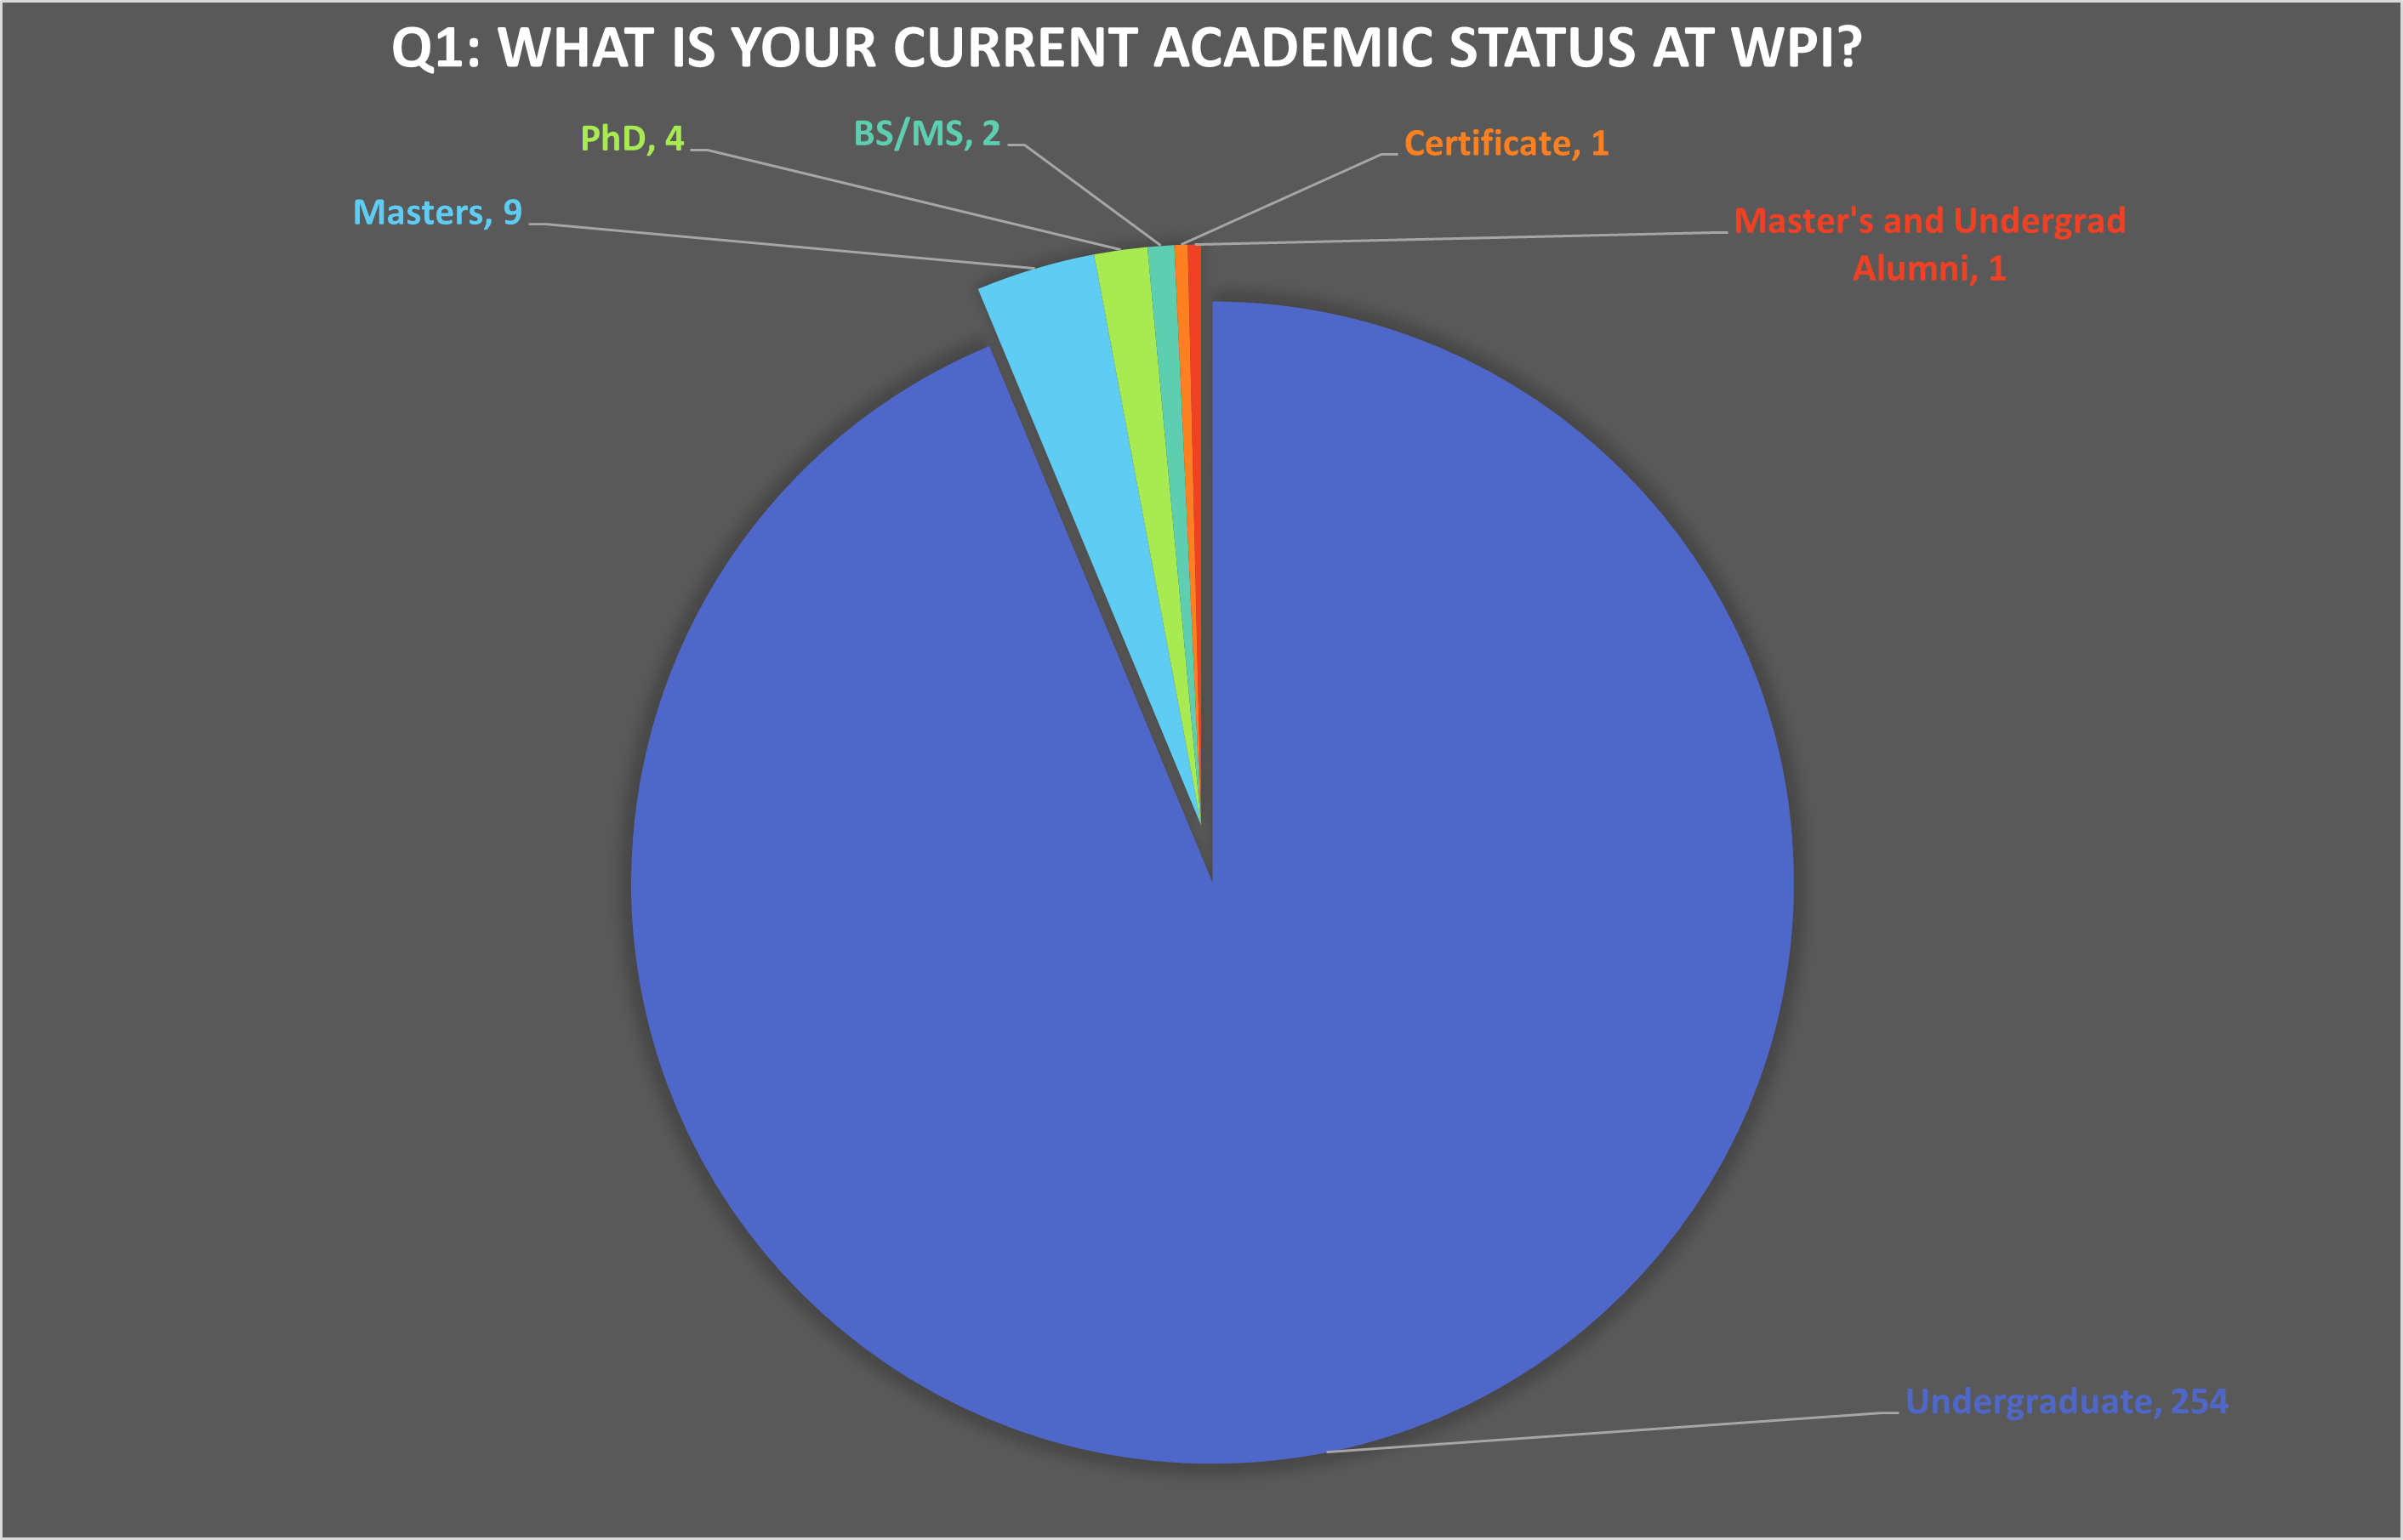
\includegraphics[width = \textwidth, height = \textheight, keepaspectratio]{assets/img/Student Survey Results Q1.png}
        \caption*{Figure 7.5.1: Academic Status of Respondents}
    \end{figure}
    \newpage
%------------------------------------------------------------------------------------------------------------------------------------------
     \begin{figure}[H]
        \hspace*{-1.75cm}
        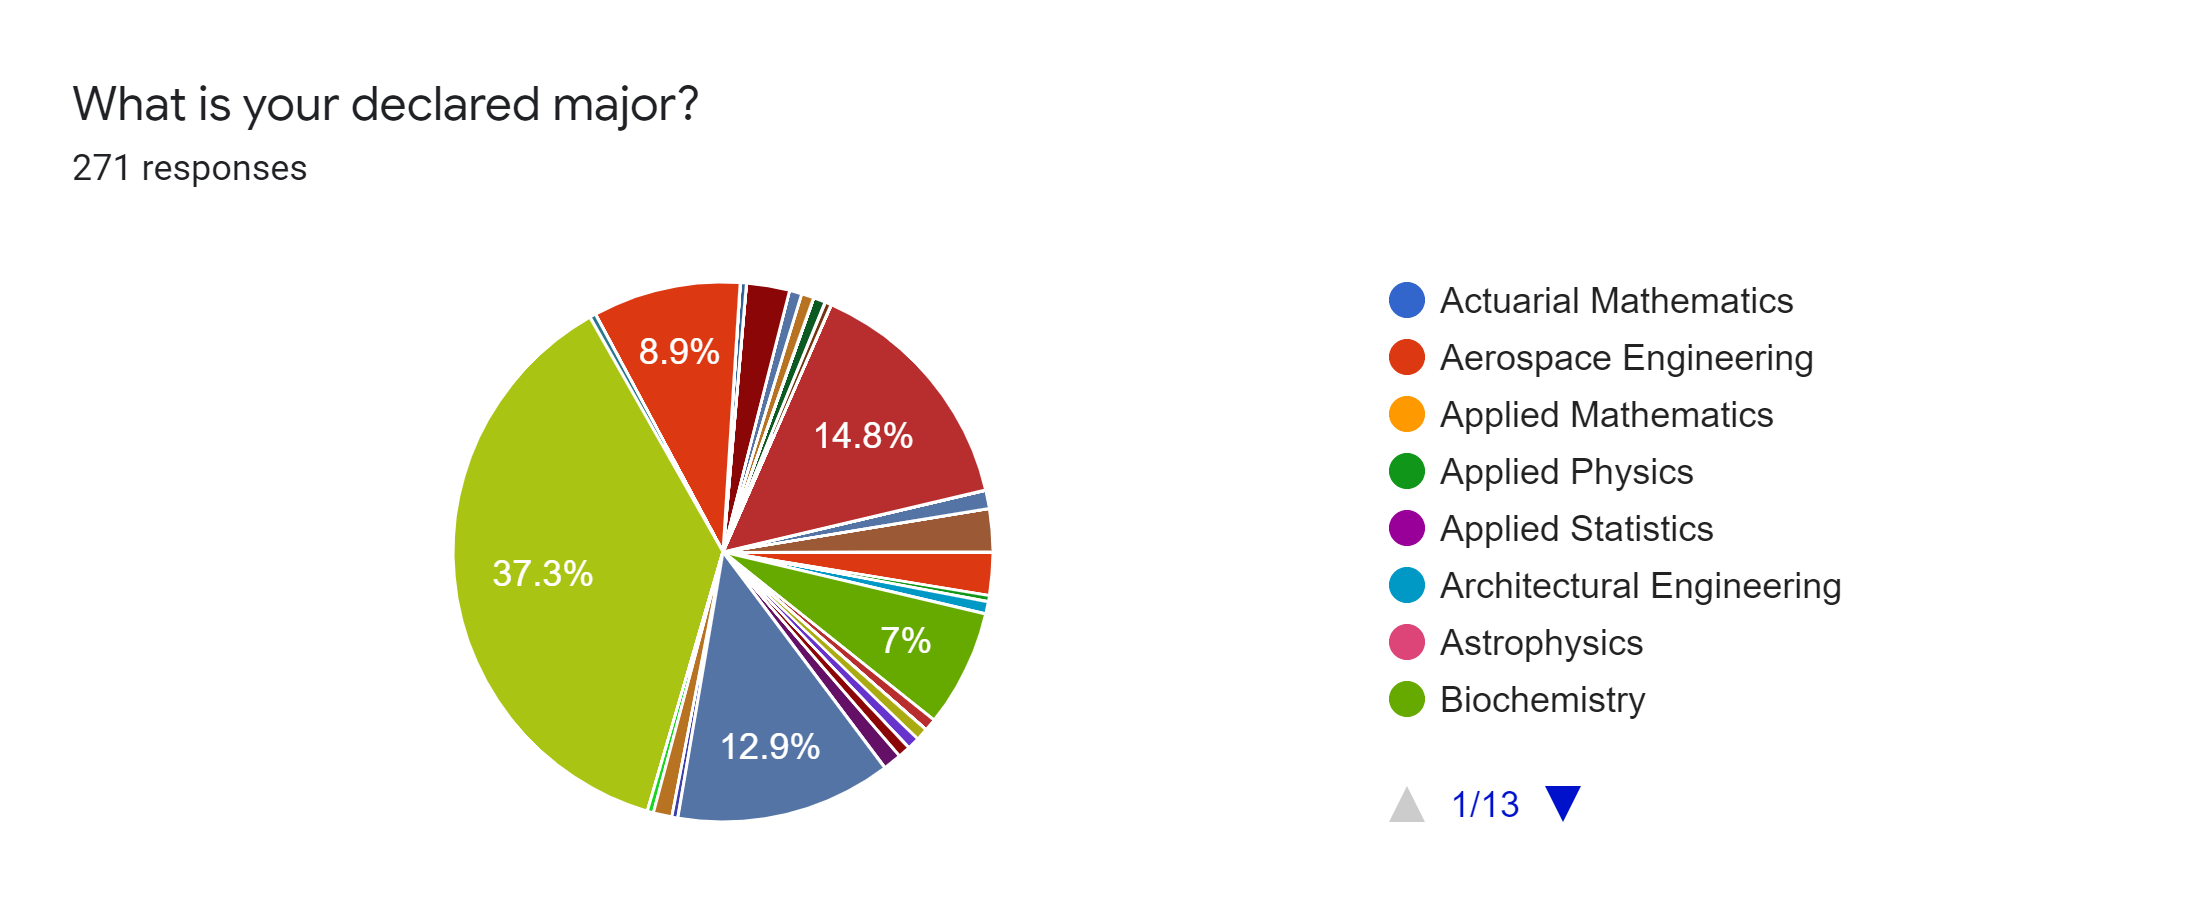
\includegraphics[scale = .4]{assets/img/Student Survey Results Q2.png}
        \caption*{Figure 7.5.2: Respondent's Declared Majors}
    \end{figure}
       \newpage
%------------------------------------------------------------------------------------------------------------------------------------------
     \begin{figure}[H]
        \centering
        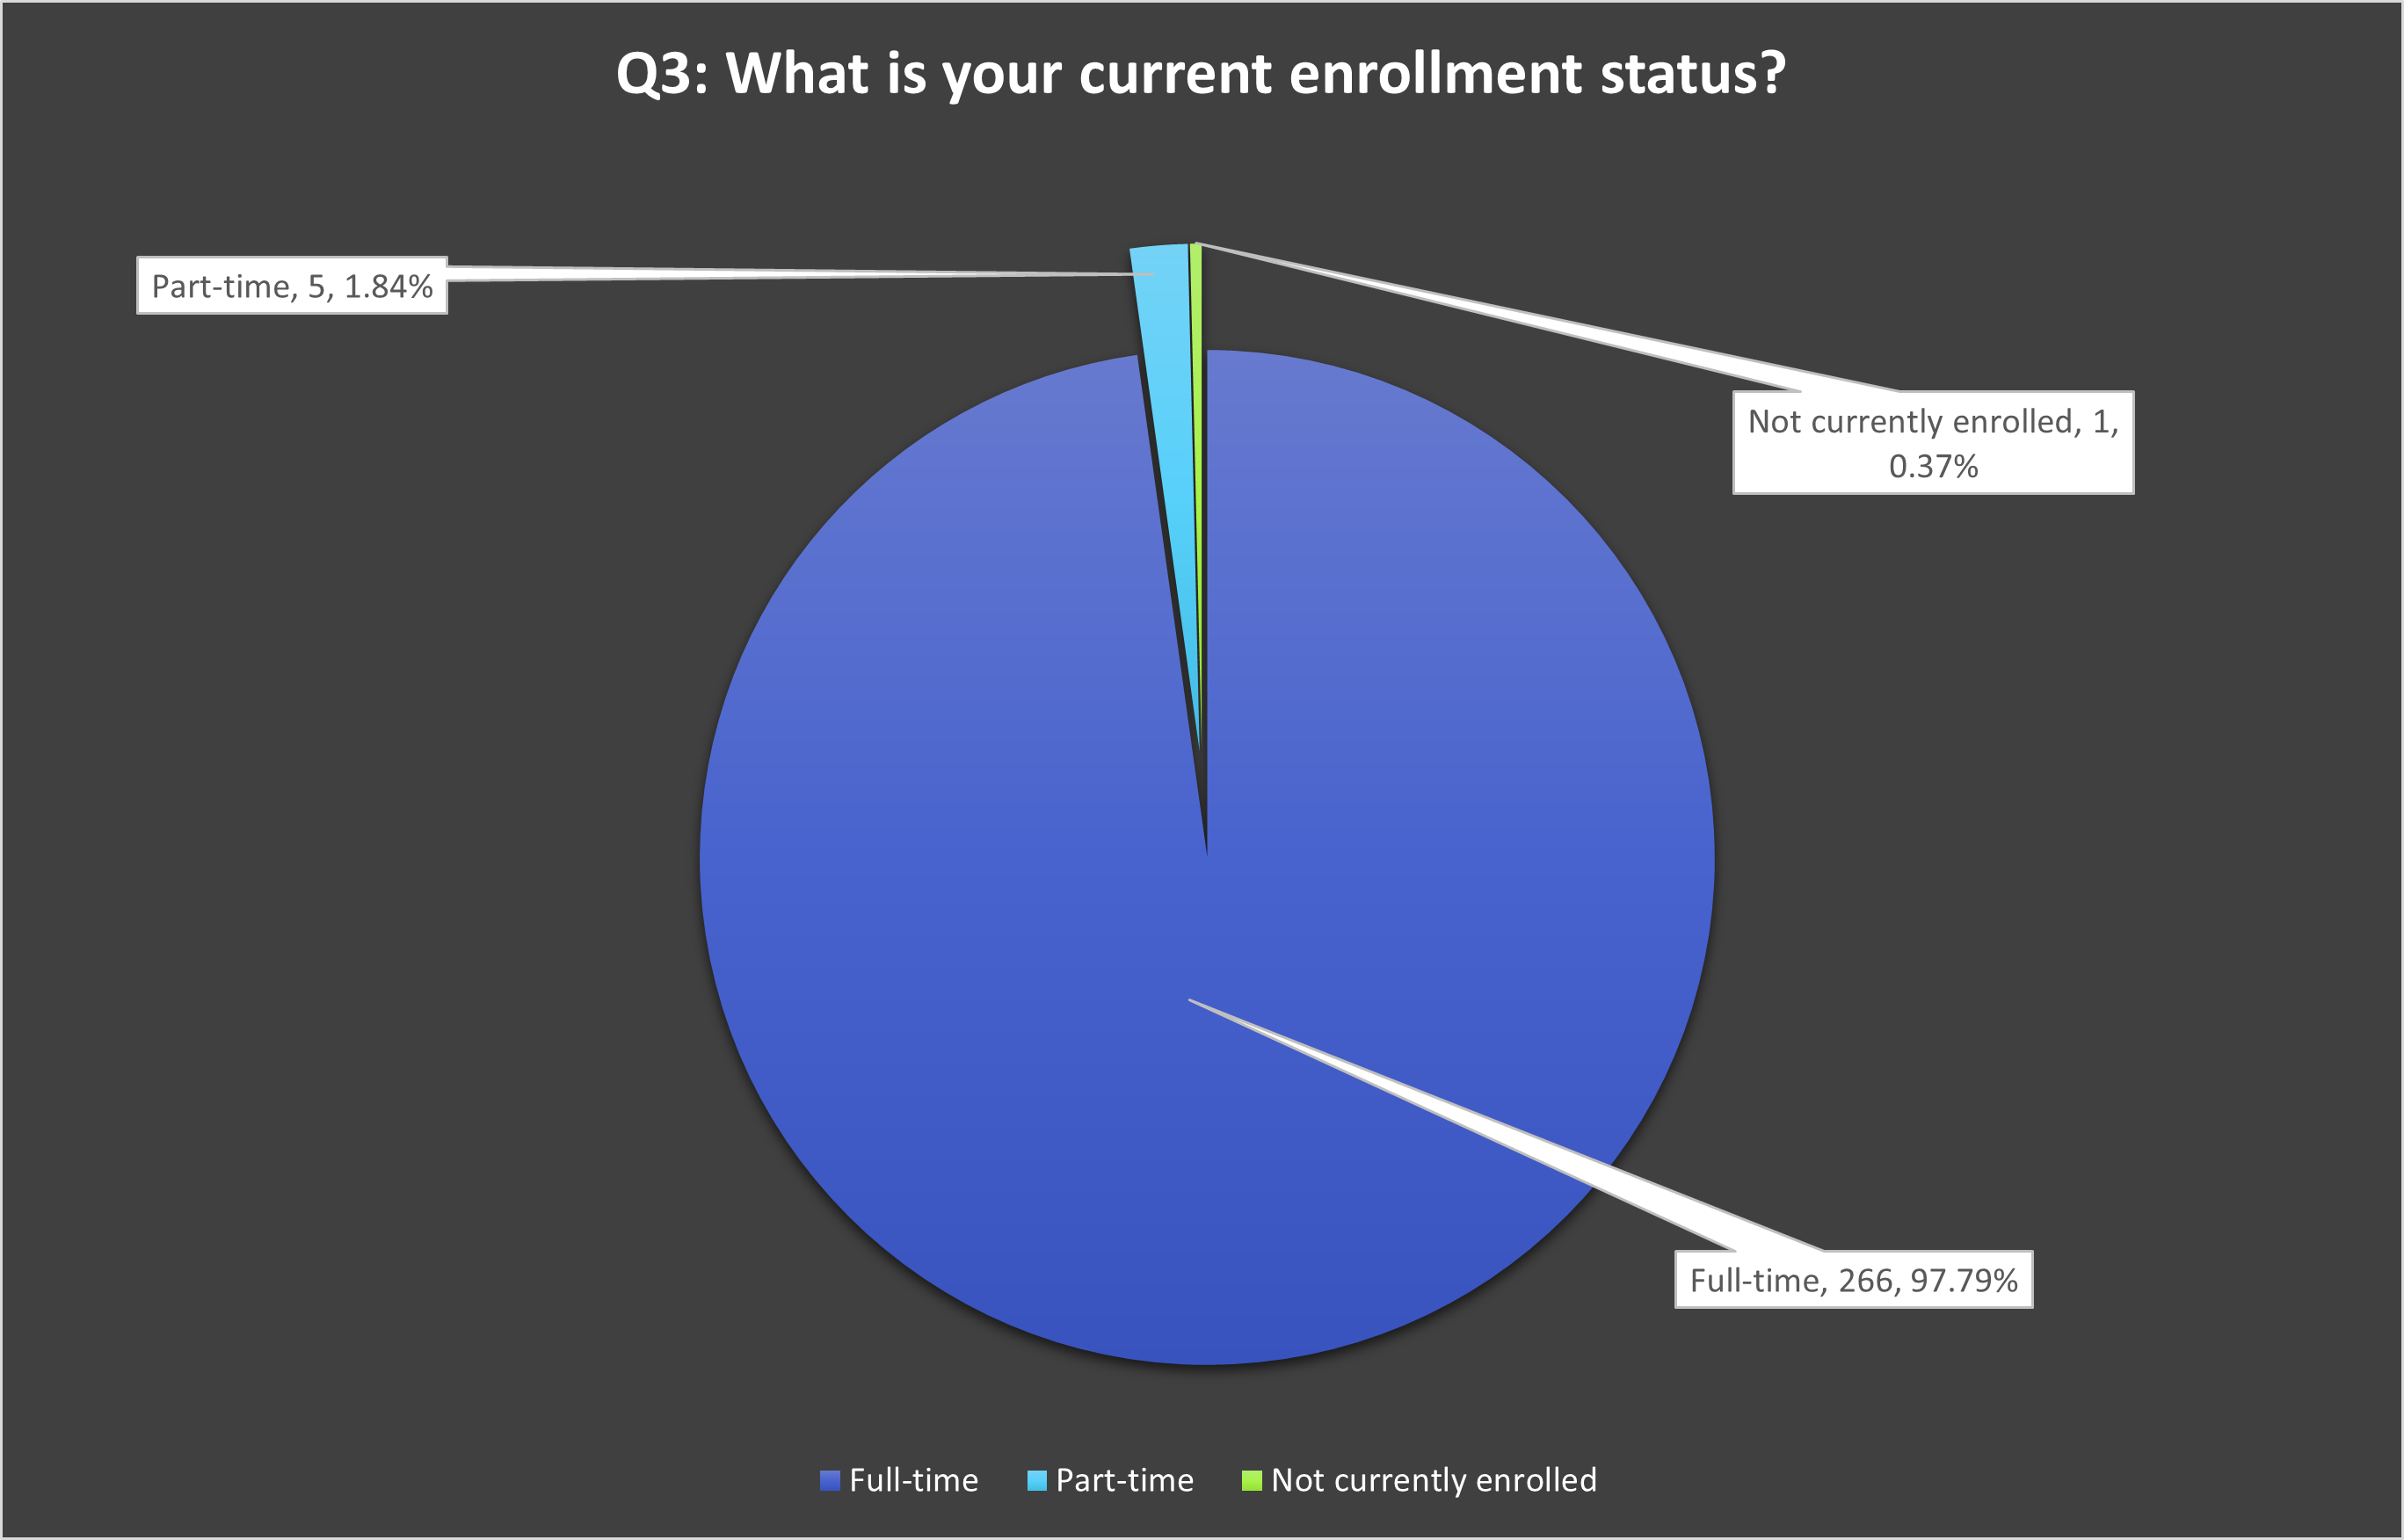
\includegraphics[width = \textwidth, height = \textheight, keepaspectratio]{assets/img/Student Survey Results Q3.png}
        \caption*{Figure 7.5.3: Respondent Enrollment Status}
    \end{figure}
       \newpage
%------------------------------------------------------------------------------------------------------------------------------------------
     \begin{figure}[H]
        \hspace*{-1.9cm}
        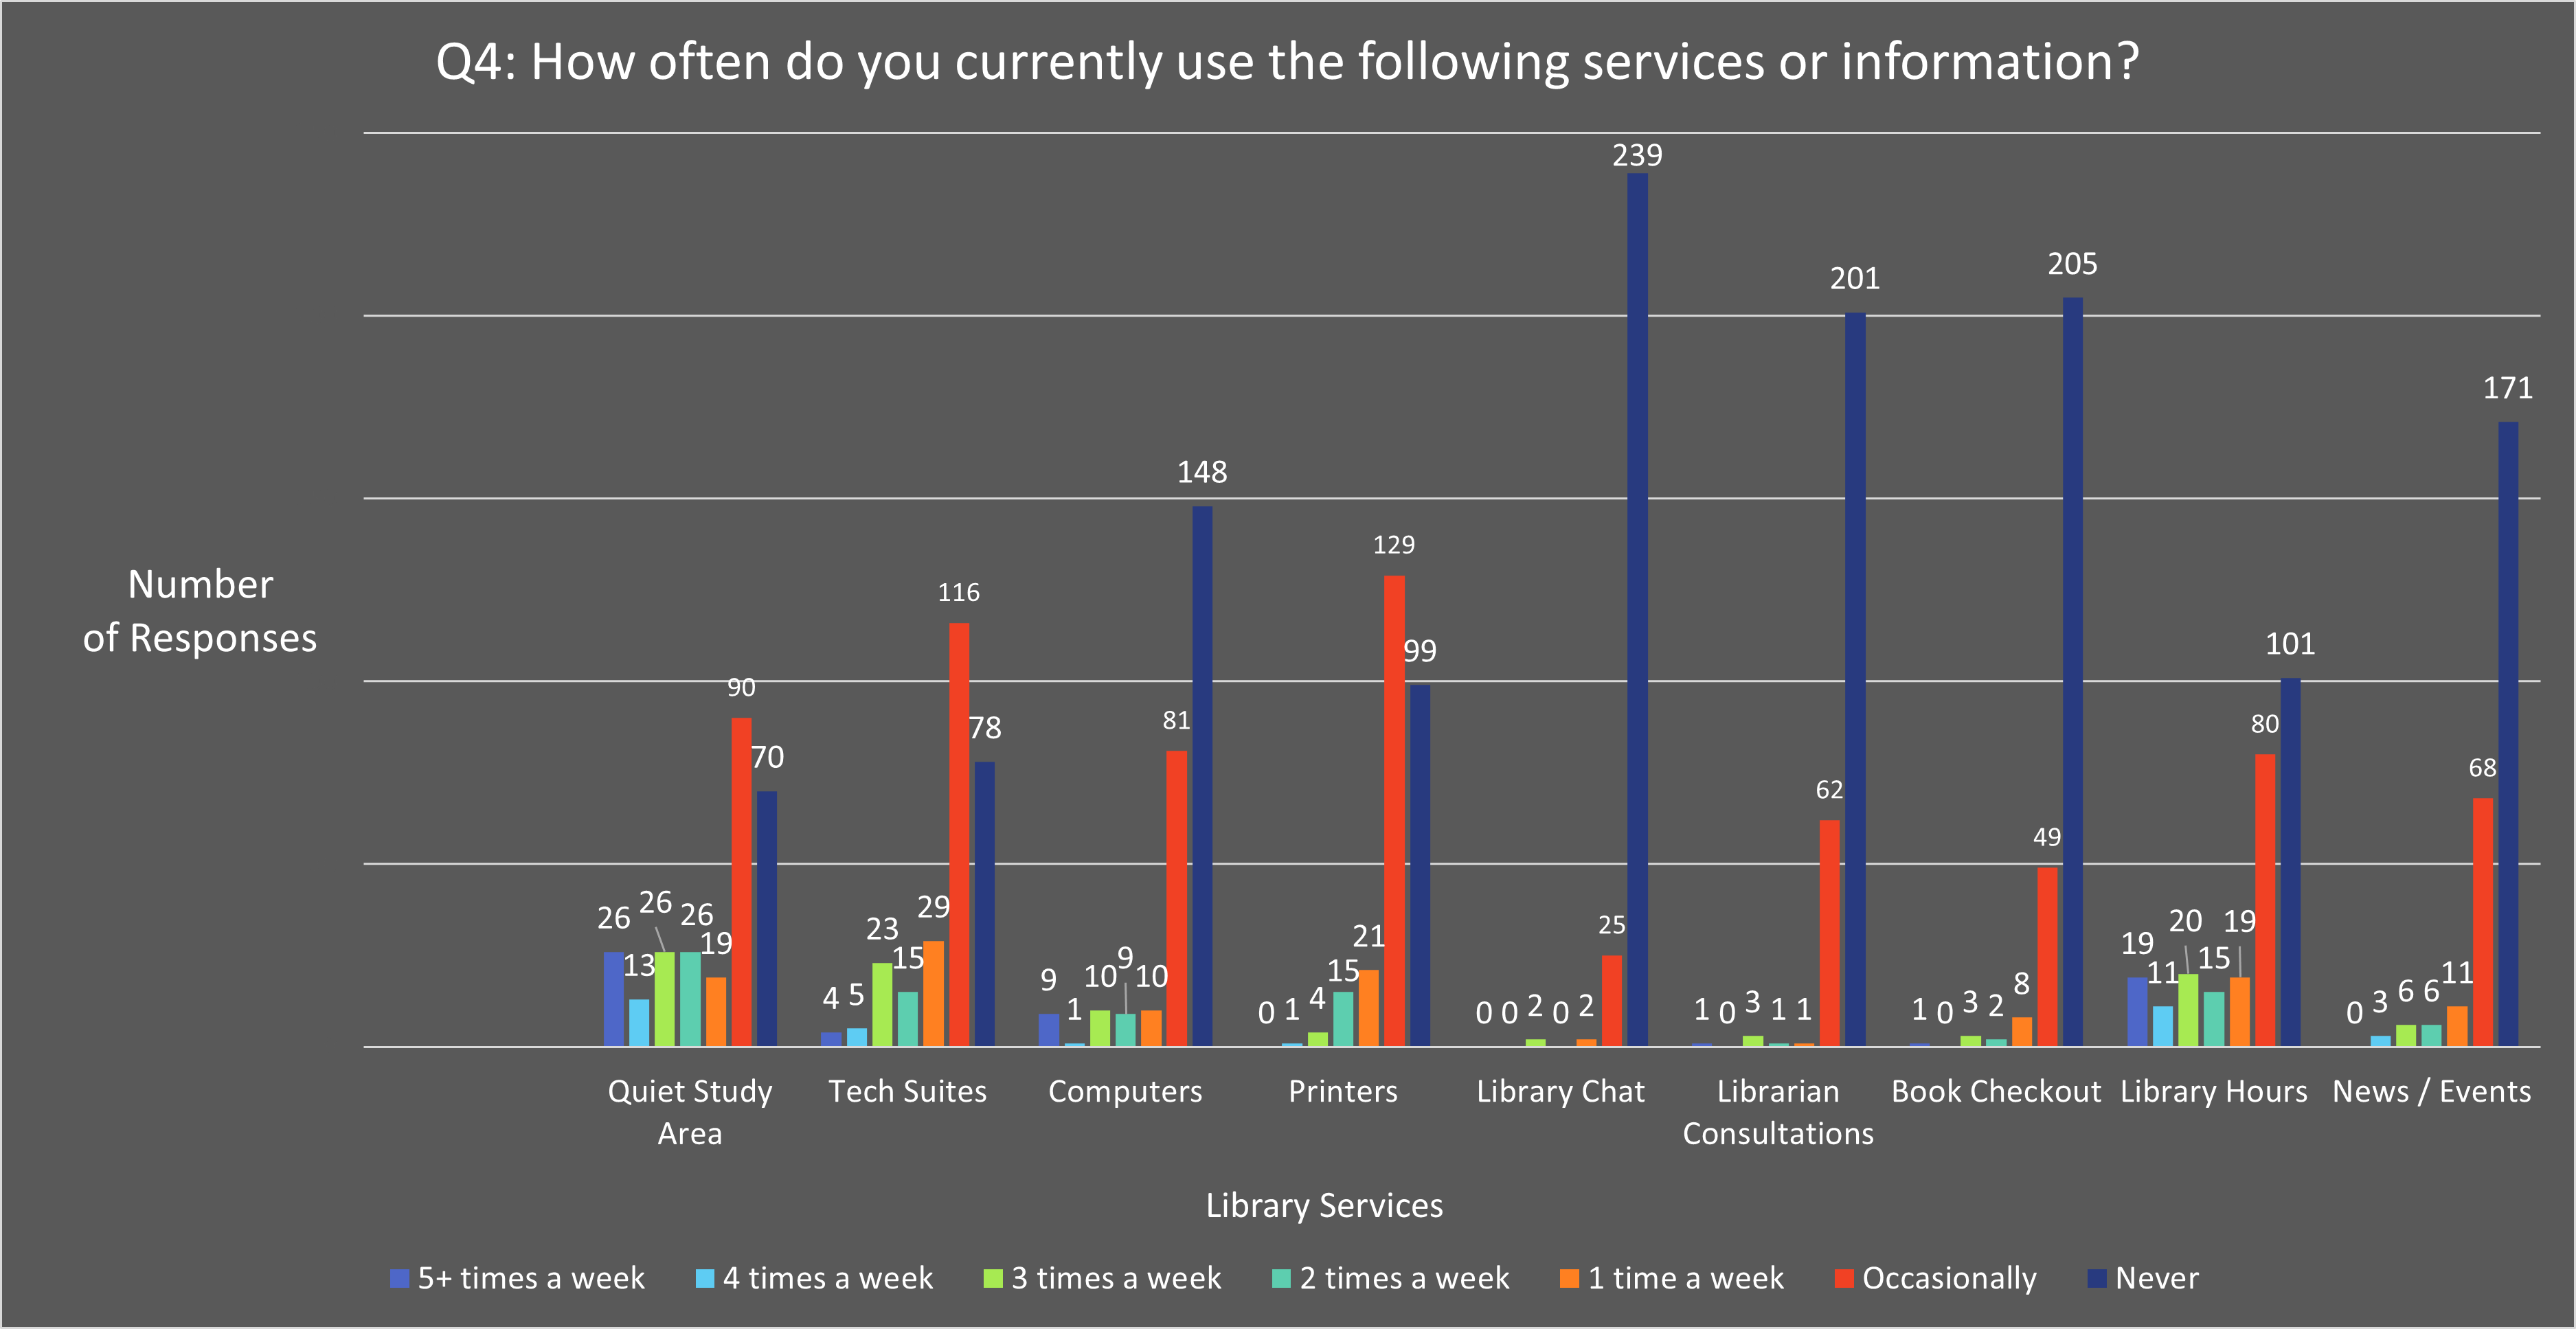
\includegraphics[scale = .7]{assets/img/Student Survey Results Q4.png}
         \caption*{Figure 7.5.4: Current Library Resource Usage}
    \end{figure}
       \newpage
%------------------------------------------------------------------------------------------------------------------------------------------
     \begin{figure}[H]
        \centering
        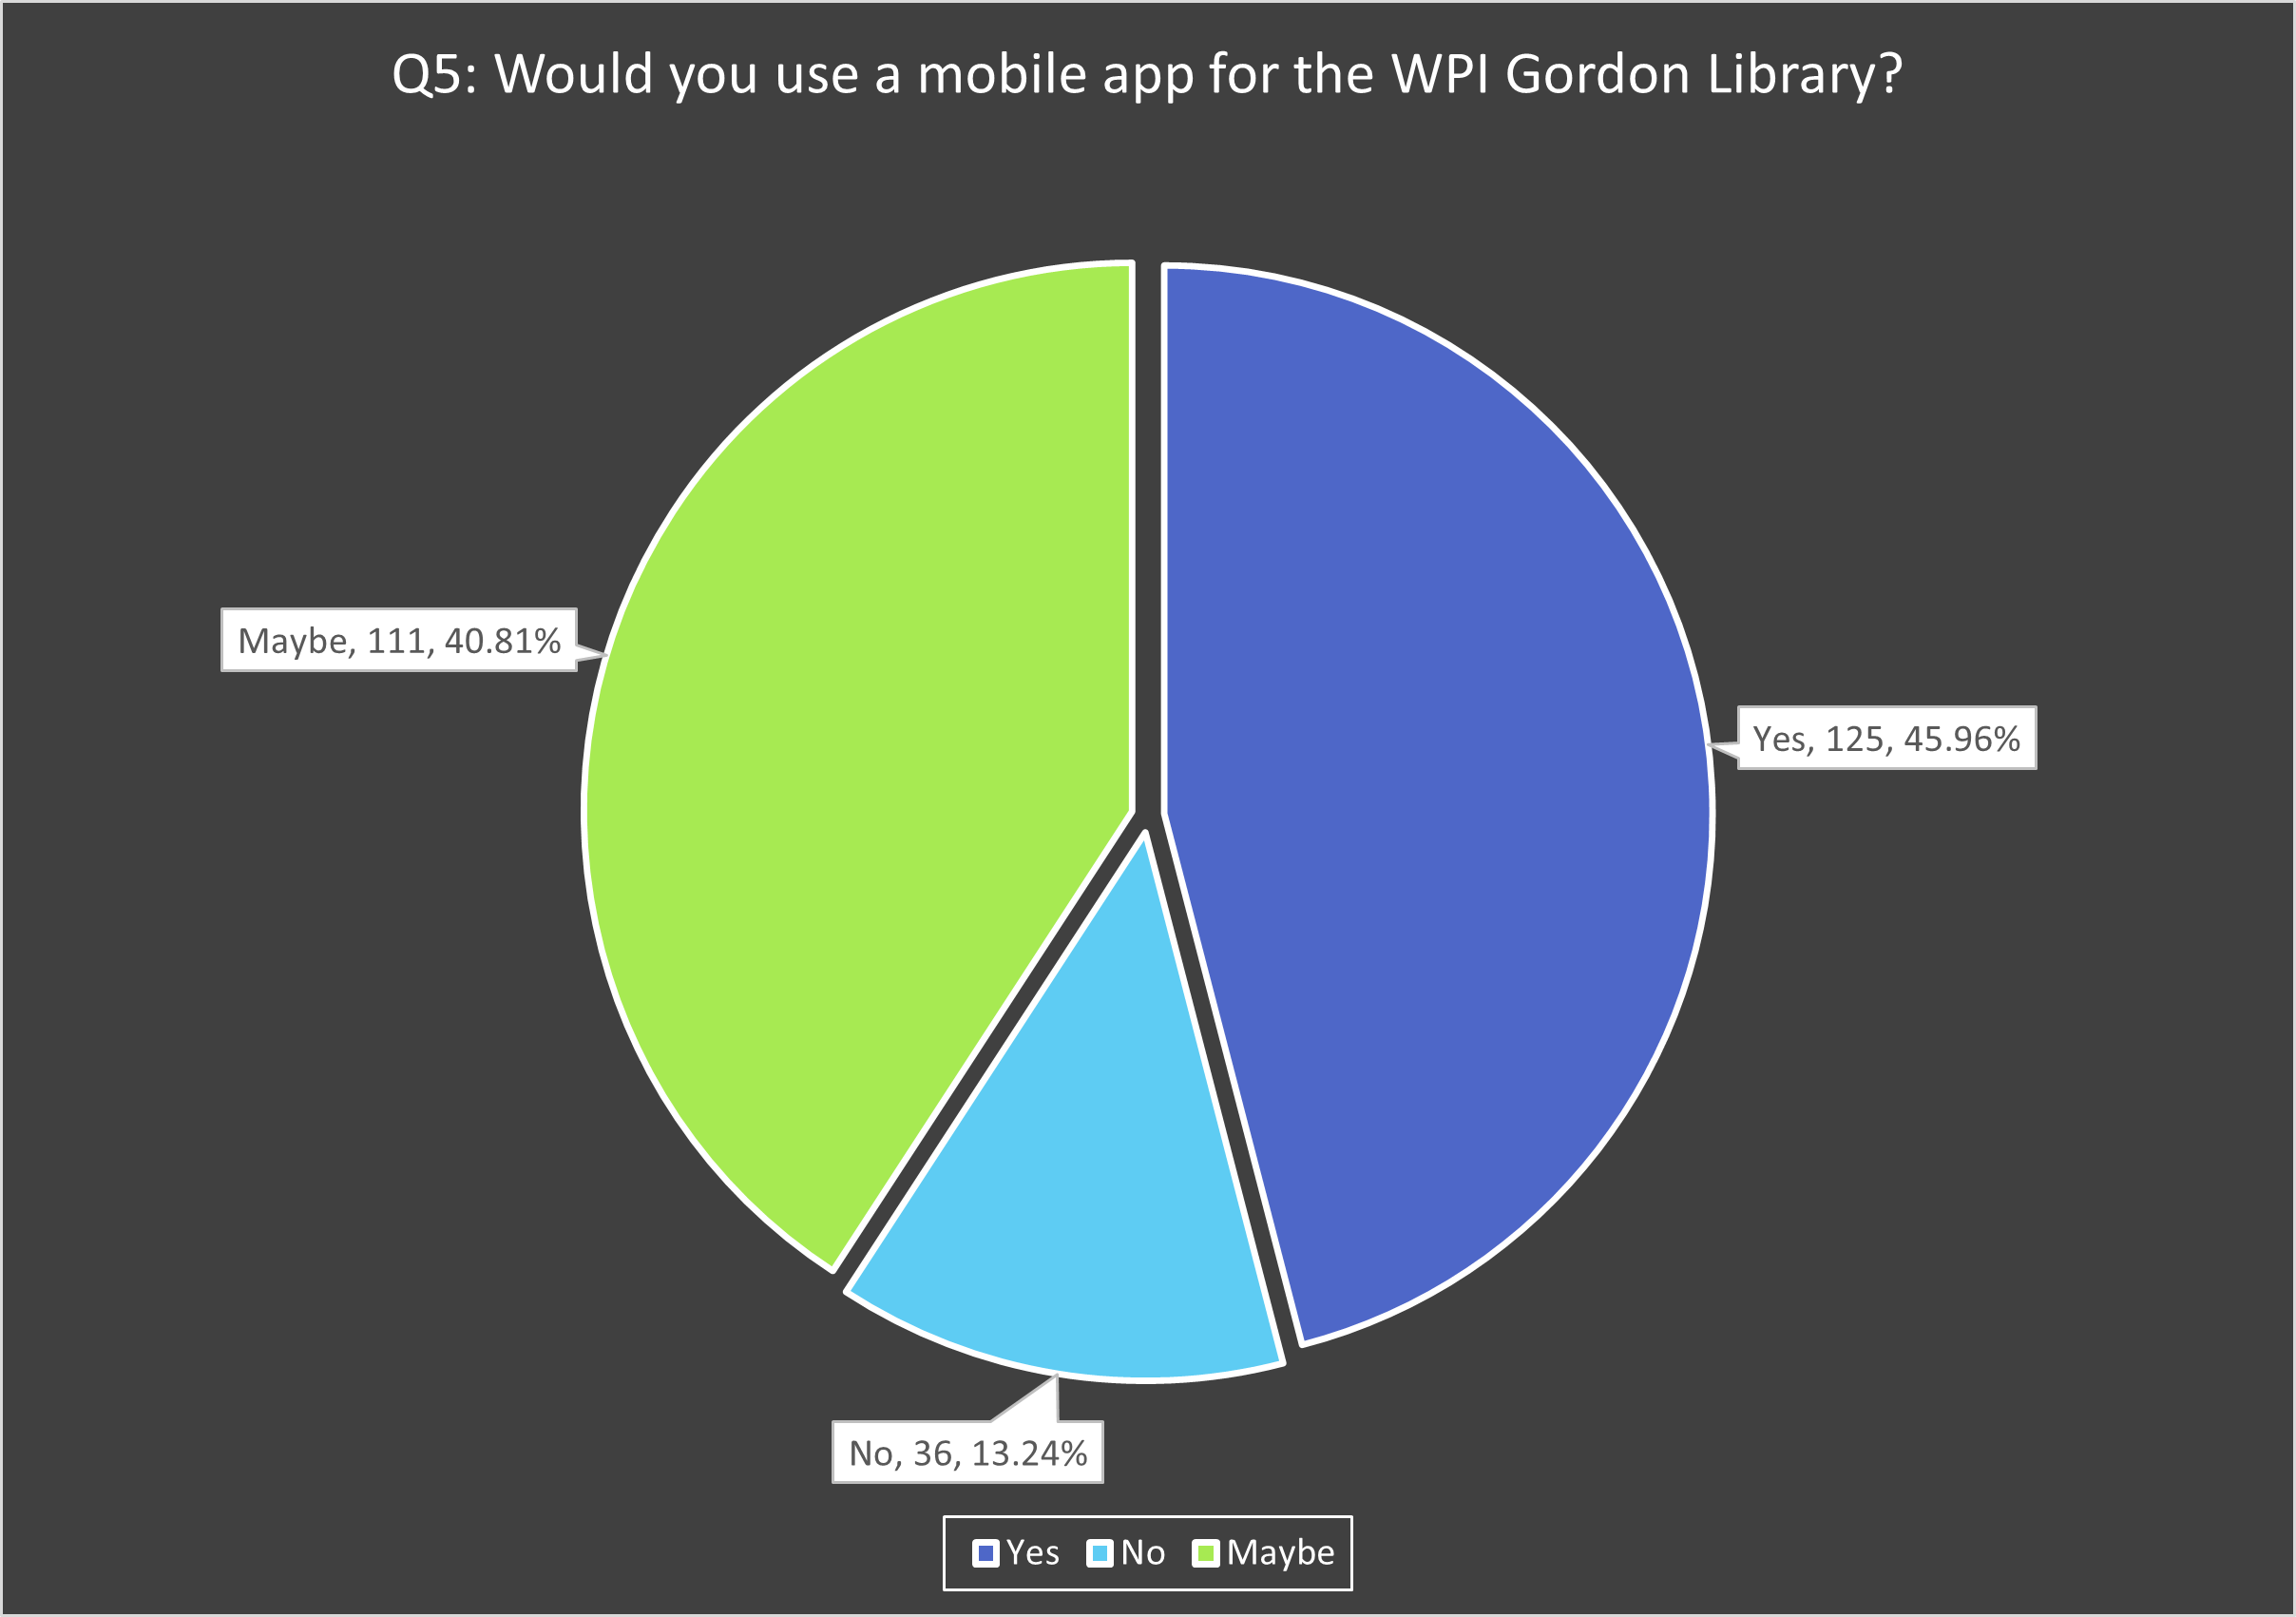
\includegraphics[width = \textwidth, height = \textheight, keepaspectratio]{assets/img/Student Survey Results Q5.png}
        \caption*{Figure 7.5.5: Mobile App Use}
    \end{figure}
       \newpage
%------------------------------------------------------------------------------------------------------------------------------------------
     \begin{figure}[H]
        \hspace*{-1.9cm}
        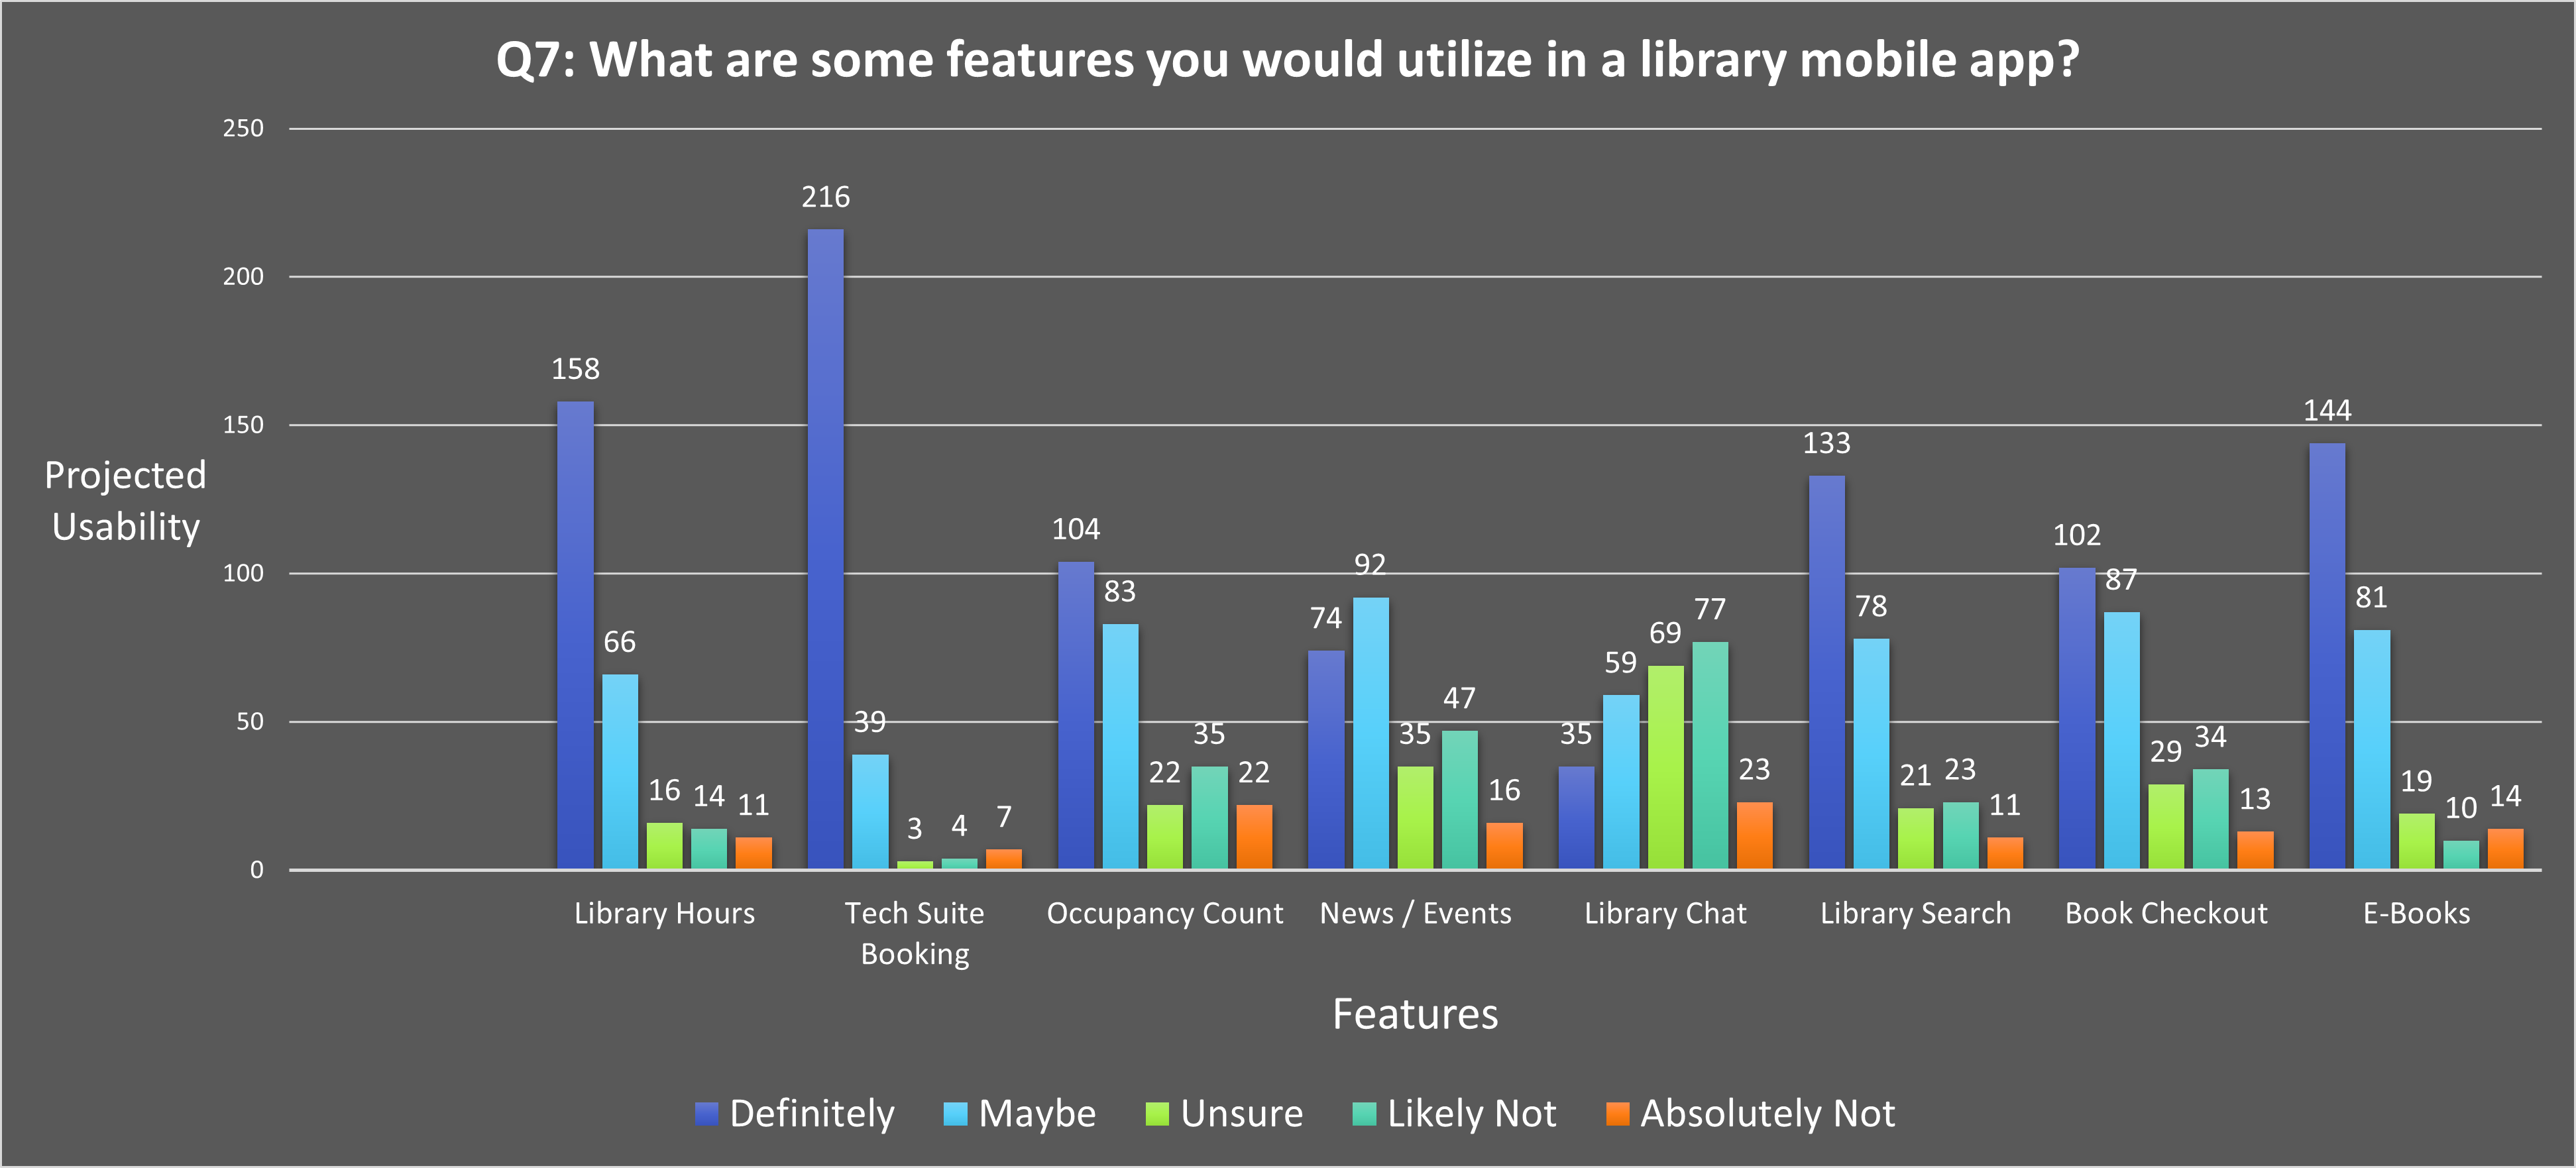
\includegraphics[scale = .68]{assets/img/Student Survey Results Q7.png}
        \caption*{Figure 7.5.6: Features That Might Be Used In A Mobile Environment}
    \end{figure}
       \newpage
%------------------------------------------------------------------------------------------------------------------------------------------
     \begin{figure}[H]
        \hspace*{-2cm}
        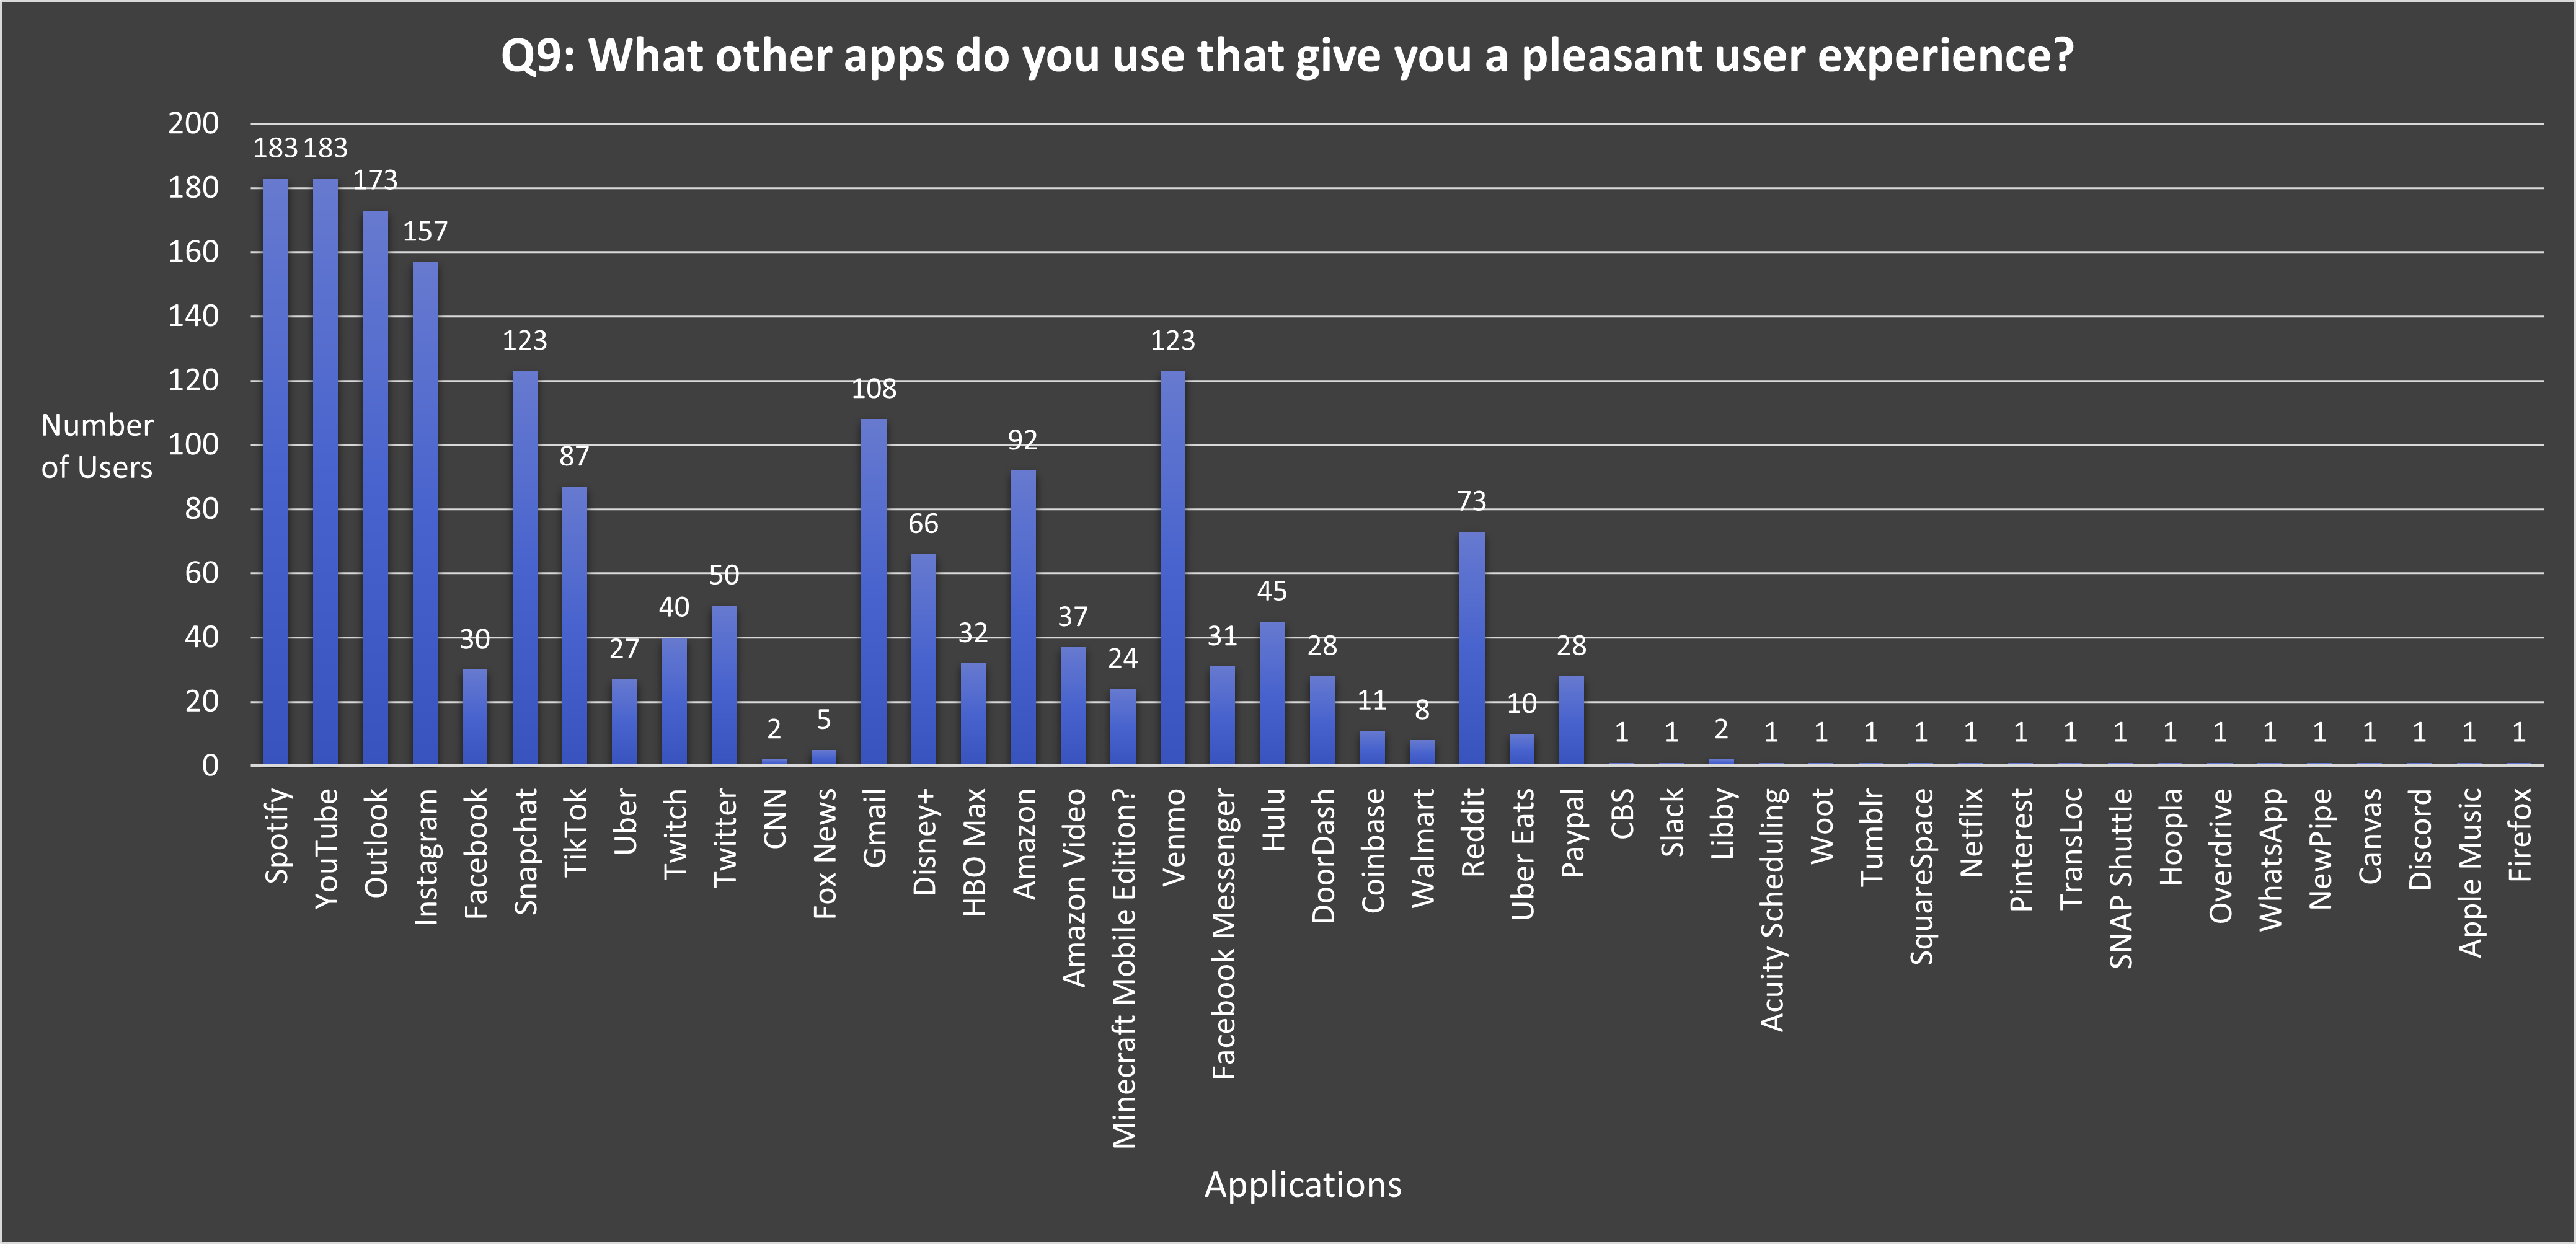
\includegraphics[scale = .64]{assets/img/Student Survey Results Q9.png}
         \caption*{Figure 7.5.7: User Experience: Other Applications Used}
    \end{figure}
       \newpage
%------------------------------------------------------------------------------------------------------------------------------------------
     \begin{figure}[H]
        \centering
        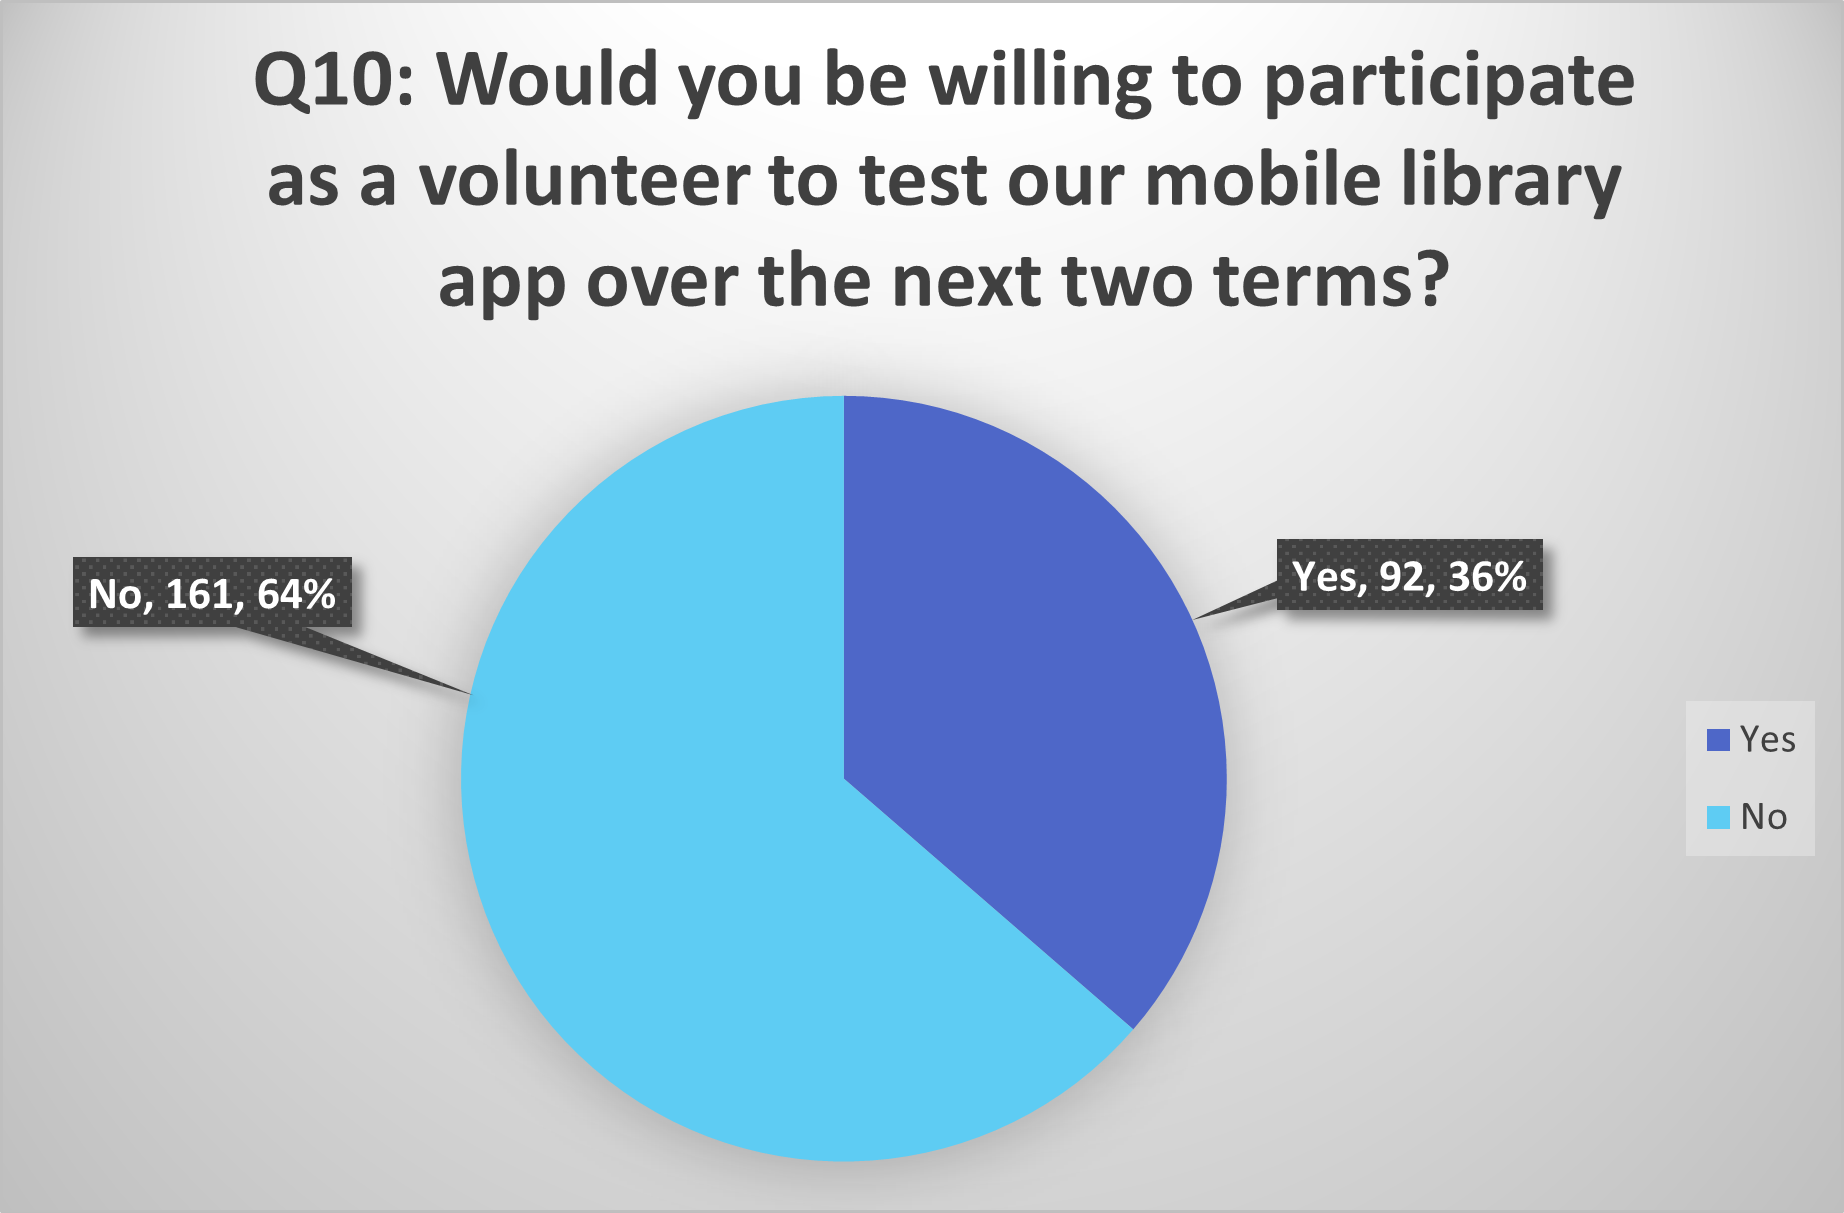
\includegraphics[width = \textwidth, height = \textheight, keepaspectratio]{assets/img/Student Survey Results Q10.png}
        \caption*{Figure 7.5.8: Volunteer Testing Participation}
    \end{figure}
%------------------------------------------------------------------------------------------------------------------------------------------

   
\end{document}
